\documentclass[12pt]{ociamthesis}

\usepackage{amssymb}
\usepackage{amsmath}
\usepackage{hyperref}
\usepackage[capitalise]{cleveref}
\usepackage{tikz}
\usepackage{xcolor}
\usepackage{algorithm}
\usepackage{algpseudocode}

\title{Differentiable Simulation for the Electrochemical
Inverse Problem}

\author{Jack Montgomery}
\college{St Anne's College}

\degree{Masters in Mathematical Sciences}
\degreedate{Trinity 2026}

\begin{document}

\baselineskip=18pt plus1pt

\setcounter{secnumdepth}{3}
\setcounter{tocdepth}{3}

\maketitle
\begin{abstract}
  We develop a differentiable forward solver for voltammetric simulation
  and integrate it with the No-U-Turn sampler to perform Bayesian
  inference over electrochemical kinetic parameters.
  A custom adjoint rule for the banded linear solve provides exact
  gradients by solving one adjoint system per timestep and caching
  only the matrix diagonals and solution vector rather than the full
  factorisation tape. This reduces the per-timestep memory
  requirements and eliminates the runtime overhead of tape traversal.
  The framework is applied to three reaction mechanisms of increasing
  complexity: a single electron transfer, a heterogeneous reaction,
  and an adsorption reaction. Under equal runtime budgets, NUTS
  produces $1.5$--$4.8\times$ the effective sample size of
  random-walk Metropolis--Hastings. Both samplers recover the true
  parameters in all cases, with posteriors revealing correlations and
  uncertainty that point estimates cannot capture.
\end{abstract}


\begin{romanpages}
  \tableofcontents
  \listoffigures
\end{romanpages}

\chapter{Introduction}\label{ch:introduction}

The inverse problem requires recovering physical parameters
from indirect measurements. This problem is ubiquitous throughout the
sciences; occurring whenever the quantities of interest cannot be observed
directly. In electrochemistry, the parameters governing a reaction at
an electrode surface must be inferred from the current response to an
applied potential. This inference is the electrochemical inverse
problem.

Predicting the current response for a given set of parameters is the
corresponding forward problem, which in the present context, reduces to
solving a diffusion PDE with kinetic boundary conditions
\cite{compton2014understanding}. Solving the inverse problem then
amounts to finding the parameters whose forward solution best
explains the observed data. The difficulty is threefold: the
mapping from parameters to current is nonlinear, distinct parameter
configurations can produce similar voltammograms, and in certain
kinetic regimes some parameters cease to influence the current altogether.
Point estimates cannot capture these difficulties. They provide no
account of uncertainty, cannot distinguish a well-constrained parameter
from one that is insensitive to the data, and do not reveal correlations
between parameters. Bayesian inference addresses this by computing the
posterior distribution conditioned on the observed
data \cite{gavaghan2018bayesian}.

The standard tool for sampling such posteriors is Markov chain Monte
Carlo. In this setting each likelihood evaluation requires a PDE solve,
so every proposed sample, whether accepted or rejected, is expensive.
Gradient-free samplers such as random-walk Metropolis--Hastings (RWMH)
explore the parameter space by undirected local proposals and
consequently waste many of these solves on rejected candidates,
particularly as the number of parameters grows. Gradient information
helps in two ways: it can initialise the sampler near a posterior mode
via optimisation; and it can inform the sampling itself
through Hamiltonian Monte Carlo (HMC), which uses the gradient to
construct long-range, low-rejection proposals.

The challenge is obtaining these gradients cheaply. Finite differences
require at least one additional forward solve per parameter and introduce
truncation error. Whereas, reverse-mode automatic differentiation computes exact
gradients at a cost bounded by a small multiple of the forward solve,
independent of parameter dimension \cite{griewank2008evaluating}.
Na\"ively taping an entire PDE solver, however, records every
intermediate of the linear solve -- elimination multipliers, modified
diagonals, partial sums -- at each timestep. We instead derive a
custom adjoint rule for the banded linear solve and
register it with the automatic differentiation framework, \emph{JAX}
\cite{jax2018github}, so that gradient computation uses only the matrix
diagonals and solution vector.

This work sits within a broader shift toward differentiable scientific
computing; Kitchin et~al.\ \cite{kitchin2025beyond} characterise
differentiable programming as a fifth paradigm for modelling in chemical
engineering. Concurrently, Chen et~al.\ \cite{chen2026differentiable}
have developed differentiable electrochemical simulators for
gradient-based parameter recovery. Our work is complementary: we
adopt a Bayesian framework rather than optimisation alone, and we
compute gradients via a custom adjoint rather than taping the full
solver. The Bayesian approach to voltammetric inference via MCMC was
established by Gavaghan et~al.\ \cite{gavaghan2018bayesian}; we
extend their framework by replacing the gradient-free sampler with
gradient-informed alternatives enabled by the differentiable solver.

This dissertation makes three contributions. First, we develop a
differentiable forward solver for voltammetric PDEs, in which a custom
adjoint rule for the banded linear system provides exact gradients at low
memory cost and generalises to the wider banded systems arising in
multi-species reactions. Second, we integrate this solver with the
No-U-Turn sampler (NUTS)~\cite{hoffman2014no}, an
extension of HMC, to obtain posterior distributions over the physical
parameters. Third, we apply the framework to three reaction
mechanisms of increasing complexity:  a single electron transfer
(3~parameters), a heterogeneous reaction (7~parameters), and an
adsorption reaction (9~parameters). We find that the advantage of
NUTS over RWMH grows with the dimensionality of the parameter space.
The methodology is developed through the single-electron-transfer
reaction, which serves as a running example; the final two chapters
apply the complete framework to the harder reactions concisely.

\chapter{Electrochemical Systems}

A typical electrochemical experiment uses an electrochemical cell to drive
reduction and oxidation (redox) reactions at the surface of a working
electrode. The cell consists of at least two electrodes immersed in an
electrolyte solution: the \emph{working electrode}, at whose surface the
reaction of interest takes place, and a \emph{counter electrode}, which
completes the circuit. A third \emph{reference electrode} is commonly
included to provide a stable, known potential against which the potential
of the working electrode is measured and controlled. A device called a
\emph{potentiostat} maintains the desired potential difference between the
working and reference electrodes, drives the current through the circuit
formed by the working and counter electrodes, and simultaneously measures
that current.

\begin{figure}
  \centering
  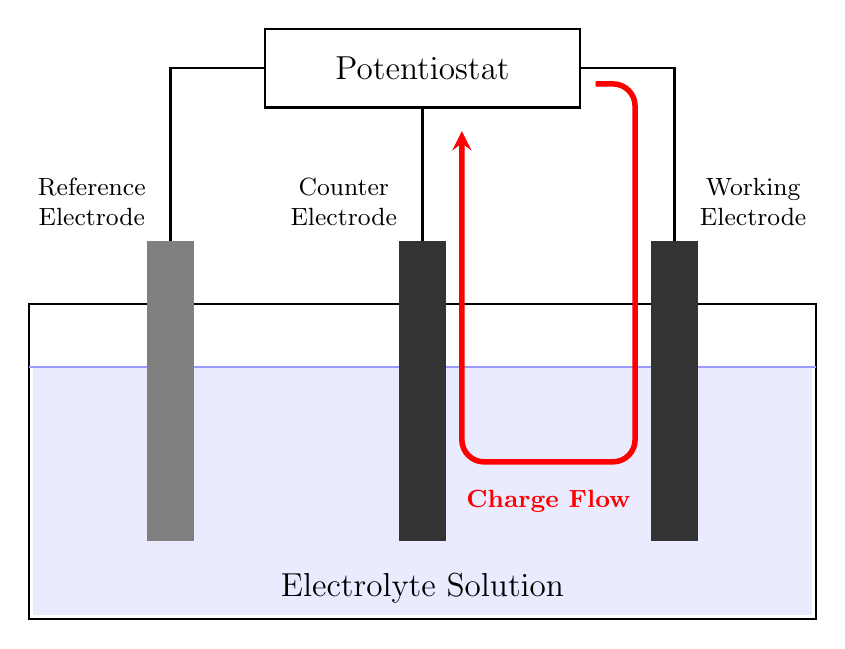
\begin{tikzpicture}[>=stealth, thick]

  % Solution vessel
  \draw[thick] (0, 0) -- (0, 4) -- (10, 4) -- (10, 0) -- cycle;
  % Solution fill
  \fill[blue!8] (0.05, 0.05) rectangle (9.95, 3.2);
  % Solution surface line
  \draw[blue!40, thick] (0, 3.2) -- (10, 3.2);
  \node[font=\large] at (5, 0.4) {Electrolyte Solution};

  % Potentiostat box
  \draw[thick, fill=white] (3, 6.5) rectangle (7, 7.5);
  \node[font=\large] at (5, 7) {Potentiostat};

  % Reference Electrode (left)
  \fill[black!50] (1.5, 1.0) rectangle (2.1, 4.8);
  \node[font=\small, align=center] at (0.8, 5.3) {Reference\\Electrode};
  % Wire from counter electrode to potentiostat
  \draw[thick] (1.8, 4.8) -- (1.8, 7) -- (3, 7);

  % Counter Electrode (centre)
  \fill[black!80] (4.7, 1.0) rectangle (5.3, 4.8);
  \node[font=\small, align=center] at (4.0, 5.3) {Counter\\Electrode};
  % Wire from reference electrode to potentiostat
  \draw[thick] (5.0, 4.8) -- (5.0, 6.5);

  % Working Electrode (right)
  \fill[black!80] (7.9, 1.0) rectangle (8.5, 4.8);
  \node[font=\small, align=center] at (9.2, 5.3) {Working\\Electrode};
  % Wire from working electrode to potentiostat
  \draw[thick] (8.2, 4.8) -- (8.2, 7) -- (7, 7);

  % Charge flow arrows (red loop)
  \draw[->, red, line width=2pt, rounded corners=8pt]
  (7.2, 6.8) -- (7.7, 6.8) -- (7.7, 2.0) -- (5.5, 2.0)
  -- (5.5, 4.0) -- (5.5, 6.2);
  \node[red, font=\small\bfseries] at (6.6, 1.5) {Charge Flow};

\end{tikzpicture}

  \caption{Schematic of a three-electrode electrochemical cell. The
    potentiostat controls the potential difference between the working
    and reference electrodes whilst driving current (red) through the
    circuit formed by the working and counter electrodes via the
  analyte solution.}
  \label{fig:electrochemical-cell}
\end{figure}

The reaction occurring at the working electrode surface depends on the
applied potential and the chemical species present in solution. In the
simplest case, a solution-phase species undergoes a single-electron redox
reaction:
\begin{equation}\label{eq:redox}
  \mathrm{A} + \mathrm{e}^{-} \rightleftharpoons \mathrm{B},
\end{equation}
where species $\mathrm{A}$ is reduced --- that is, it gains one electron ---
to form species $\mathrm{B}$. The reverse process, in which $\mathrm{B}$
loses an electron to regenerate $\mathrm{A}$, is the corresponding
oxidation. Throughout this chapter we restrict attention to this
single-electron ($n = 1$) process and adopt the convention that a
\emph{positive} current corresponds to net reduction (cathodic current).

\section{Voltammetry}

Voltammetry is the class of electroanalytical techniques in which the
potential applied to the working electrode is varied in a prescribed
manner and the resulting current is recorded. Because the current is
directly related to the rate of the electrochemical reaction at the
electrode surface, the current--potential curve --- called a
\emph{voltammogram} --- encodes information about the kinetics of the
redox process as well as the transport of chemical species in solution.

In a cyclic voltammetry (CV) experiment the applied potential is swept
linearly with time from a starting potential~$E_i$, chosen so that the
overpotential is insufficient to drive any significant reaction, towards
more negative values (for a reduction) until a vertex potential~$E_v$ is
reached. The vertex potential is chosen sufficiently beyond the formal
potential of the redox couple that the reaction is driven to completion at
the electrode surface; it serves only as the turning point of the sweep.
The potential is then swept back to~$E_i$, reversing the direction of
electron transfer and reforming~$\mathrm{A}$. This triangular waveform is
illustrated in the left panel of \cref{fig:potential-voltammagram}.

Throughout this process the current $I$ is recorded. Plotting the current
against the applied potential gives the voltammogram shown in the right
panel of \cref{fig:potential-voltammagram}. The forward sweep produces
a reduction (cathodic) peak as the potential moves through the range at
which $\mathrm{A}$ is converted to $\mathrm{B}$; the return sweep produces
an oxidation (anodic) peak as $\mathrm{B}$ is reconverted to $\mathrm{A}$.

The peak shape arises from competition between two rate-limiting
processes. During the early part of the forward sweep the applied
potential is positive relative to the formal potential of the redox
couple, so there is insufficient driving force to reduce $\mathrm{A}$ and
negligible current flows. As the potential is swept to more negative
values the reduction reaction becomes progressively more
thermodynamically favourable and the current increases: during this rising
portion the system is under \emph{kinetic control}, meaning that the rate
of electron transfer at the electrode surface is the rate-limiting step.
Eventually the concentration of~$\mathrm{A}$ in the immediate vicinity of
the electrode is depleted to near zero and the current reaches a peak.
Beyond this point the current decays despite the continued increase in
thermodynamic driving force, because the reaction has passed into
\emph{diffusional control}: the rate at which fresh~$\mathrm{A}$ can be
transported to the electrode by diffusion is now the limiting factor.

\begin{figure}
  \begin{center}
    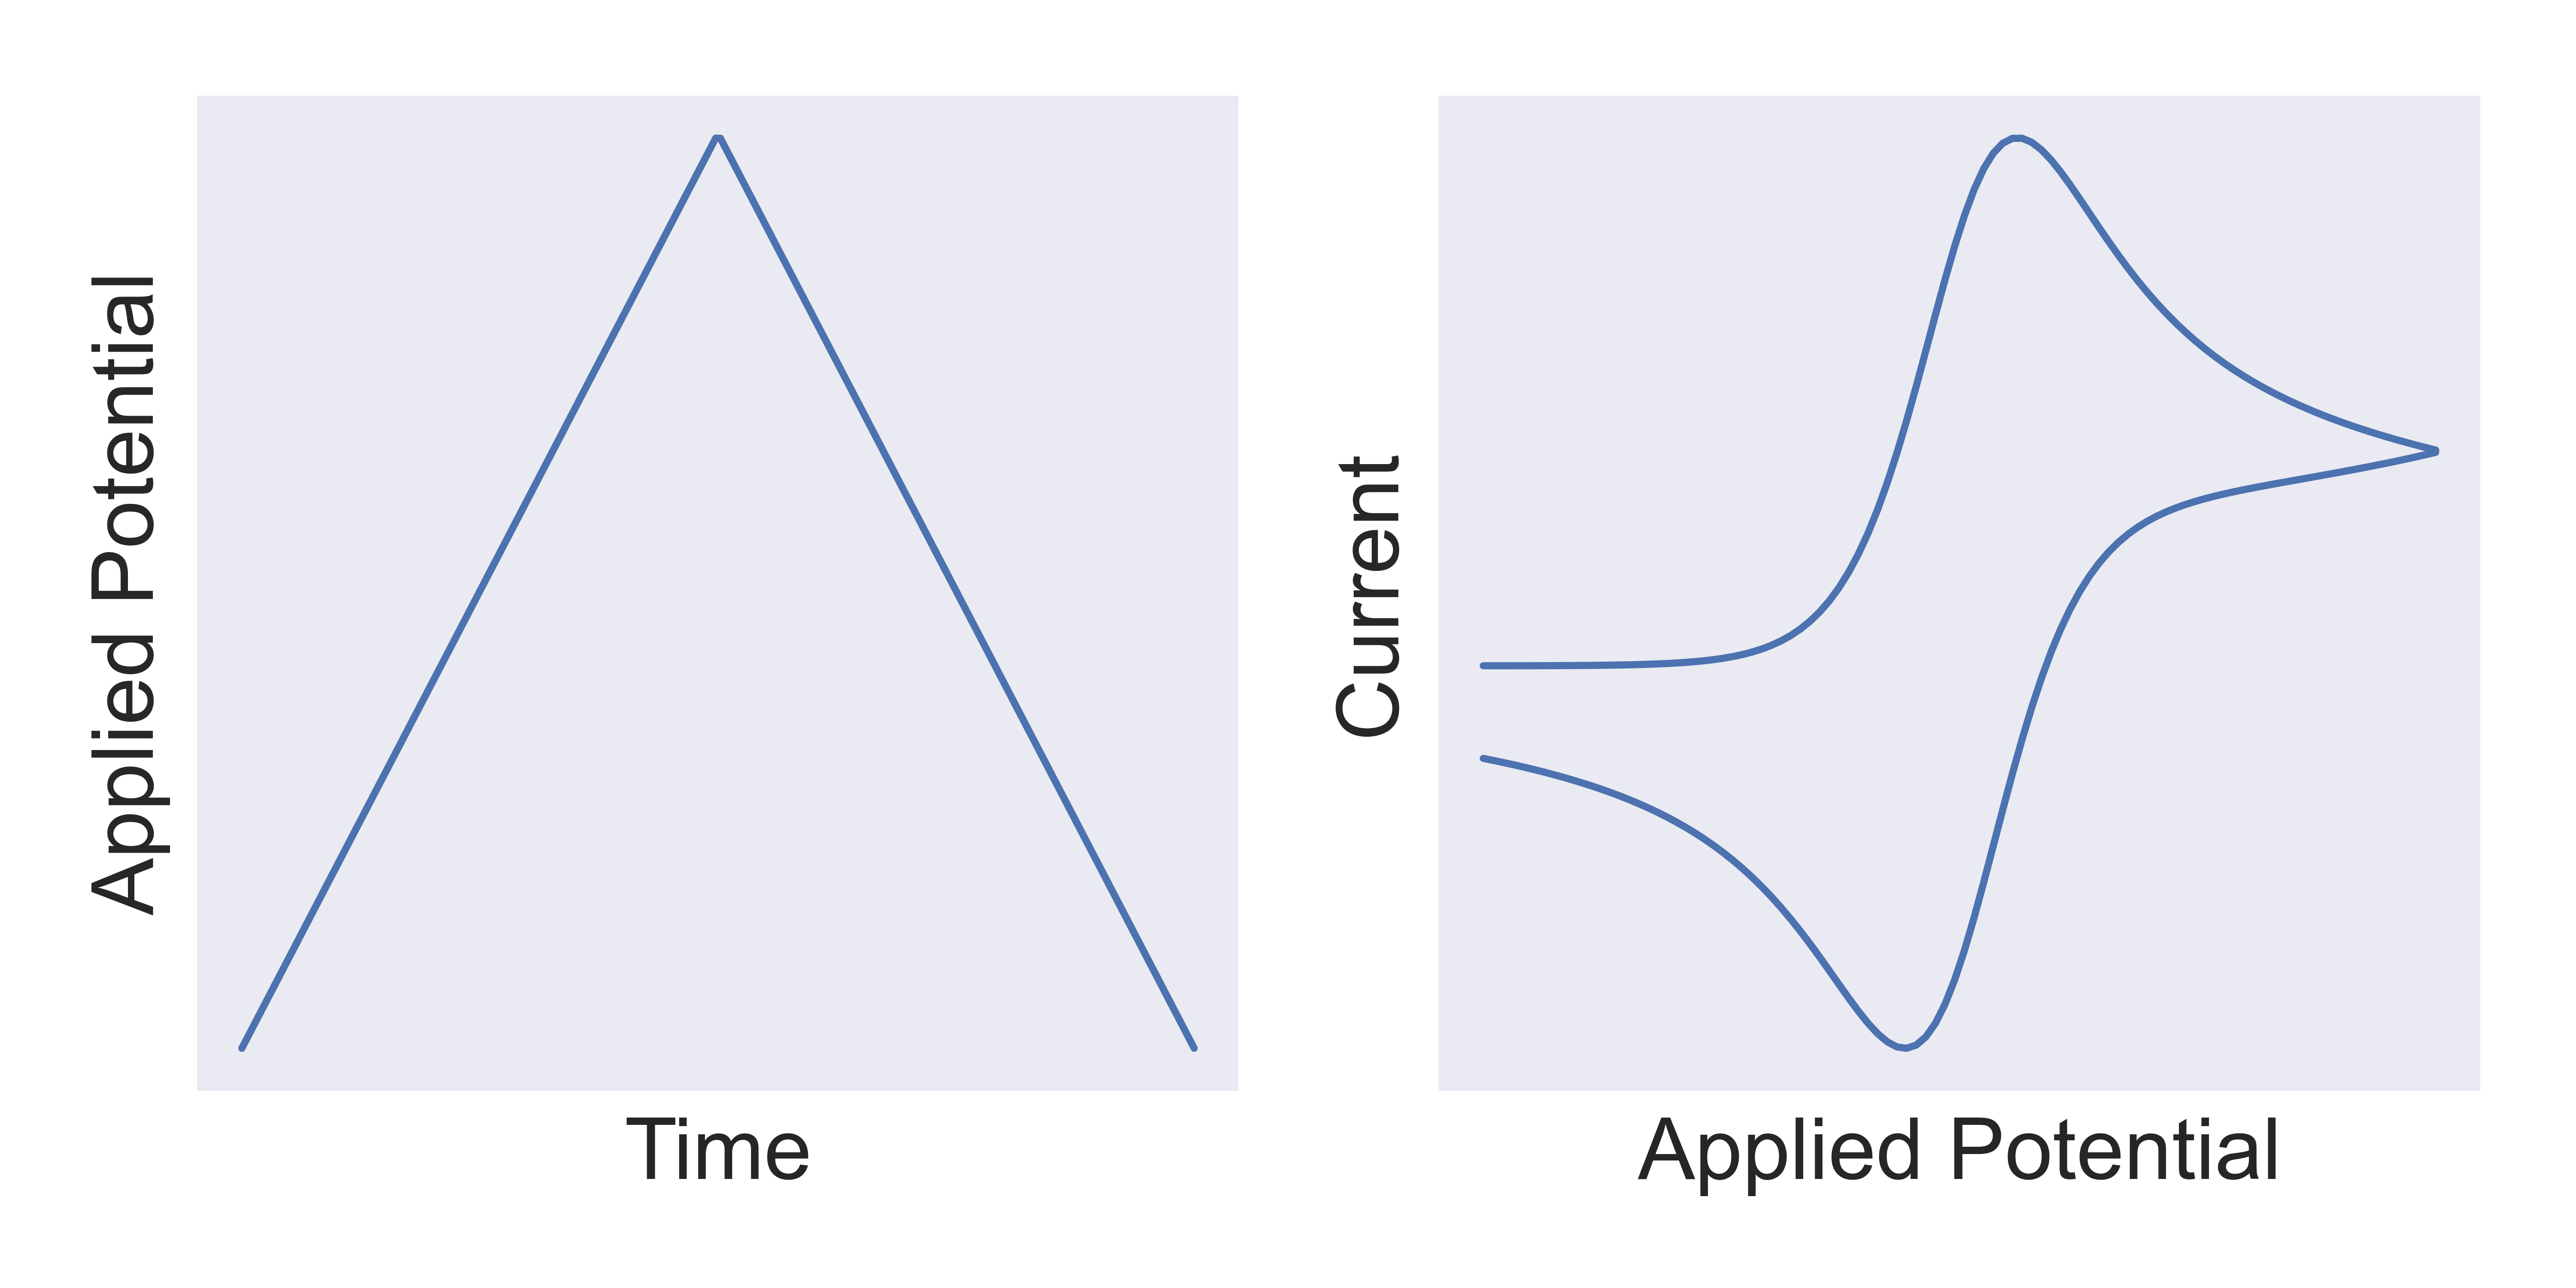
\includegraphics[width=0.8\textwidth]{figures/applied-potential-and-voltammagram.png}
  \end{center}
  \caption[Applied potential and voltammogram example]{Left: the triangular
    potential waveform applied in a cyclic voltammetry experiment. Right:
    the resulting reversible reaction's voltammogram showing the cathodic
    (reduction) peak which occurs on the forward sweep and the anodic
  (oxidation) peak which occurs on the reverse sweep.}
  \label{fig:potential-voltammagram}
\end{figure}

Cyclic Voltammetry is particularly useful because the position, shape, and
relative heights of the peaks provide a signature of the
electrochemical process. The potential at which each peak occurs is related
to the formal potential $E^{\circ}_f$, and the separation between
the cathodic and anodic peaks carries information about the electrode
kinetics, as discussed in \cref{sec:electrode-kinetics}.

The \emph{scan rate} $\nu$ $(\mathrm{V\,s^{-1}})$ is the constant rate at
which the potential is swept, defined as
\begin{equation}
  \nu = \frac{dE}{dt}.
  \label{eq:scan_rate}
\end{equation}
The scan rate is an important experimental parameter: faster scans probe
shorter timescales and can resolve kinetic processes that would otherwise
reach equilibrium on a slower scan, whilst slower scans allow more time for
diffusion and can reveal coupled chemical reactions.

\section{Mathematical Description}

We now formulate the governing equations for the system. The first
assumption we make is that we have a ``macro''-electrode: specifically, we
consider a planar disc electrode of radius~$\epsilon$, whose characteristic
dimension is much larger than the distance over which species can diffuse
on the timescale of the experiment. As a consequence, edge effects are
negligible and we can model only the diffusion perpendicular to the
electrode surface, reducing the problem to one spatial dimension.

\begin{figure}
  \centering
  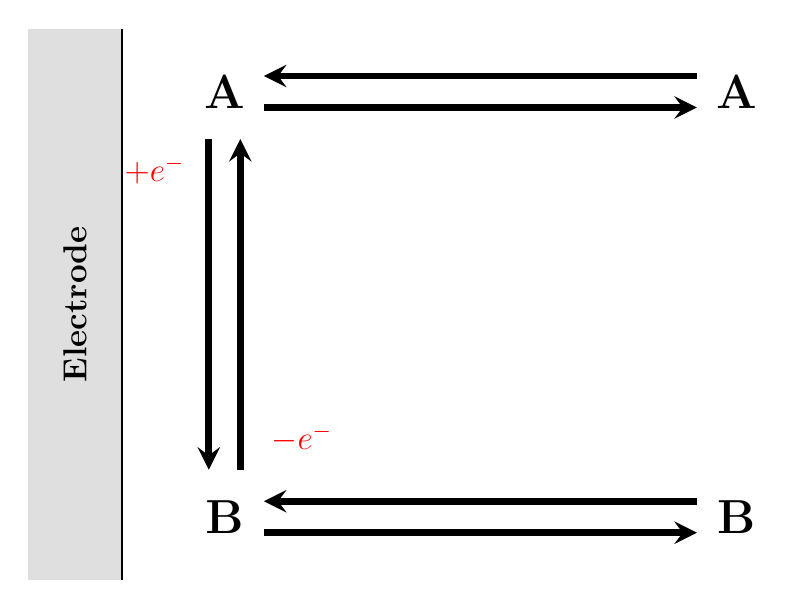
\begin{tikzpicture}[>=stealth, thick]
  % Electrode block
  \fill[gray!25] (-1.2, -1) rectangle (0, 6);
  \draw[thick] (0, -1) -- (0, 6);
  \node[rotate=90, font=\large\bfseries] at (-0.6, 2.5) {Electrode};
  % Species A row (top)
  \node[font=\LARGE\bfseries] at (1.3, 5.2) {A};
  \node[font=\LARGE\bfseries] at (7.8, 5.2) {A};
  % A: arrows
  \draw[->, line width=2.5pt] (7.3, 5.4) -- (1.8, 5.4);
  \draw[->, line width=2.5pt] (1.8, 5.0) -- (7.3, 5.0);
  % Species B row (bottom)
  \node[font=\LARGE\bfseries] at (1.3, -0.2) {B};
  \node[font=\LARGE\bfseries] at (7.8, -0.2) {B};
  % B: arrows
  \draw[->, line width=2.5pt] (7.3, 0.0) -- (1.8, 0.0);
  \draw[->, line width=2.5pt] (1.8, -0.4) -- (7.3, -0.4);
  % Electron transfer arrows
  \draw[->, line width=2.5pt] (1.1, 4.6) -- (1.1, 0.4);
  \node[left, font=\large] at (2.8, 0.8) {\textcolor{red}{$-e^-$}};
  \draw[->, line width=2.5pt] (1.5, 0.4) -- (1.5, 4.6);
  \node[right, font=\large] at (-0.1, 4.2) {\textcolor{red}{$+e^-$}};
\end{tikzpicture}

  \caption{Schematic of the one-dimensional electrode reaction. Species
    $\mathrm{A}$ diffuses from the bulk solution towards the electrode
    surface, where it is reduced ($+e^-$) to form species $\mathrm{B}$.
    The reverse oxidation ($-e^-$) converts $\mathrm{B}$ back to
    $\mathrm{A}$. Species $\mathrm{B}$ diffuses away from the electrode
  into the bulk.}
\end{figure}

\subsection{Diffusion: Fick's Second Law}\label{sec:diffusion}

We model the transport of species in quiescent (unstirred) solution using
Fick's second law~\cite{crank1979mathematics}, which describes the
evolution of a concentration field $c(x,t)$ due to diffusion. For the
couple $\mathrm{A}/\mathrm{B}$ on the planar
electrode we have the system
\begin{equation}
  \begin{aligned}
    \frac{\partial c_A}{\partial t}
    &= D_A \frac{\partial^2 c_A}{\partial x^2}, \\
    \frac{\partial c_B}{\partial t}
    &= D_B \frac{\partial^2 c_B}{\partial x^2},
  \end{aligned}
  \label{eq:diffusion}
\end{equation}
where $D_A$ and $D_B$ $(\mathrm{m^2\,s^{-1}})$ are the diffusion
coefficients of the respective species and $x$ denotes the distance from
the electrode surface. Each equation is a linear parabolic partial
differential equation defined on the semi-infinite domain $x \geq 0$.

\subsection{Fick's First Law and Electrode
Kinetics}\label{sec:electrode-kinetics}

Fick's first law~\cite{crank1979mathematics} states that the diffusive
flux through a plane normal to the $x$-axis at a point $x^*$ is
proportional to the concentration gradient at that point:
\begin{equation}
  j_{x^*} = -D\left(\frac{\partial c}{\partial x}\right)\bigg|_{x = x^*},
  \label{eq:ficks-first}
\end{equation}
where the negative sign indicates that the flux is directed down the
concentration gradient.

The rate at which the electrode reaction~\cref{eq:redox} proceeds is
governed by the applied potential. The standard model for electrode
kinetics is the Butler--Volmer equation~\cite{dickinson2020butler}, which
relates the applied potential $E(t)$ to the net flux of $\mathrm{A}$ at
the electrode surface:
\begin{equation}
  j_{0, A} = k_0 \left[ c_A(t,0)\,
    e^{-\alpha \frac{F}{\mathcal{R}\mathcal{T}} (E(t) - E^0_f)}
    - c_B(t,0)\,
    e^{(1-\alpha) \frac{F}{\mathcal{R}\mathcal{T}} (E(t) - E^0_f)}
  \right],
  \label{eq:butler-volmer}
\end{equation}
where $k_0$ $(\mathrm{m\,s^{-1}})$ is the standard rate constant, $\alpha
\in (0,1)$ is the transfer coefficient, $F$ is Faraday's constant,
$\mathcal{R}$ is the
universal gas constant, and $\mathcal{T}$ is the absolute temperature.
The quantity $E(t) - E^0_f$ is the overpotential, measuring the
deviation of the applied potential from the formal potential. The first
exponential term represents the reduction contribution: a negative
overpotential ($E(t) < E^0_f$) enhances this term and drives the
conversion of $\mathrm{A}$ to $\mathrm{B}$. The second exponential
represents the oxidation contribution, which dominates when the
overpotential is positive. In the limit of large $k_0$ the exponential
terms force the surface concentrations towards thermodynamic equilibrium
and the system exhibits reversible behaviour; when $k_0$ is small the
reaction is kinetically limited and the flux is directly proportional
to~$k_0$, giving irreversible behaviour.

Combining \cref{eq:ficks-first,eq:butler-volmer} at the electrode surface
($x = 0$) yields a Neumann boundary condition for the diffusion
equations:
\begin{equation}
  -D_A\left(\frac{\partial c_A}{\partial x}\right)\bigg|_{x = 0} =
  k_0 \left[ c_A(t,0)\,
    e^{-\alpha \frac{F}{\mathcal{R}\mathcal{T}} (E(t) - E^0_f)}
    - c_B(t,0)\,
    e^{(1-\alpha) \frac{F}{\mathcal{R}\mathcal{T}} (E(t) - E^0_f)}
  \right].
  \label{eq:electrode-boundary-condition}
\end{equation}
Conservation of mass at the electrode surface requires that whatever is
consumed of $\mathrm{A}$ is produced as $\mathrm{B}$, and vice versa. Since
we consider a single-electron process with no homogeneous reactions in
solution, this is simply stoichiometric conservation:
\begin{equation}
  D_B\left(\frac{\partial c_B}{\partial x}\right)\bigg|_{x = 0} =
  -D_A\left(\frac{\partial c_A}{\partial x}\right)\bigg|_{x = 0}.
  \label{eq:mass-conservation}
\end{equation}

\subsection{Boundary and Initial Conditions}

At the start of the experiment we assume that $\mathrm{A}$ is at some
bulk concentration $c_A^*$ and that $\mathrm{B}$ is at bulk concentration
$c_B^*$:
\begin{equation}
  \begin{aligned}
    c_A(0, x) &= c_A^*, \\
    c_B(0, x) &= c_B^*.
  \end{aligned}
  \label{eq:initial-conditions}
\end{equation}
Far from the electrode surface, the redox reaction has no effect on the
concentrations, so the bulk values are recovered:
\begin{equation}
  \begin{aligned}
    c_A(t, x) &\to c_A^* \quad \text{as } x \to \infty, \\
    c_B(t, x) &\to c_B^* \quad \text{as } x \to \infty.
  \end{aligned}
  \label{eq:infinite-boundary-condition}
\end{equation}

\subsection{Current}

The primary experimental observable of a voltammetry experiment is the
current measured by the potentiostat. At any instant the current for the
single-electron reduction of species $\mathrm{A}$ is
\begin{equation}
  I = F A_{\mathrm{el}}\, j_{0, A},
  \label{eq:current}
\end{equation}
where $A_{\mathrm{el}} = \pi\epsilon^2$ is the area of the disc electrode
and $j_{0, A}$ is the net flux of species $\mathrm{A}$ at the electrode
surface, which is proportional to the concentration gradient at that point
by Fick's first law~\cref{eq:ficks-first}. Under our sign convention a
positive $j_{0,A}$ corresponds to net consumption of~$\mathrm{A}$ at the
surface (reduction) and hence a positive current. Computing the current
therefore reduces to evaluating how $j_{0, A}$ evolves in time.

\section{Non-Dimensionalisation}

The combination of
\cref{eq:diffusion,eq:electrode-boundary-condition,eq:mass-conservation,%
eq:initial-conditions,eq:infinite-boundary-condition} constitutes an
initial-boundary value problem. It is advantageous to solve a
non-dimensional version of this problem: the results of a single
non-dimensional simulation can be rescaled to any combination of physical
parameters without rerunning the computation. We non-dimensionalise in the
standard way, scaling concentrations by the bulk concentration
of~$\mathrm{A}$, diffusion coefficients by~$D_A$, lengths by the
electrode radius~$\epsilon$, and potentials by the thermal voltage
$\mathcal{R}\mathcal{T}/F$.

We present a summary of the normalisation in \cref{tab:normalisation}.

\begin{table}[ht]
  \centering
  \begin{tabular}{ll}
    \hline
    Parameter & Normalisation \\
    \hline
    concentration & $C_j = c_j / c_{\mathrm{A}}^*$ \\
    diffusion coefficient & $d_j = D_j / D_{\mathrm{A}}$ \\
    spatial coordinate & $X = x / \epsilon$ \\
    time & $T = D_{\mathrm{A}} t / \epsilon^2$ \\
    applied potential & $\theta = (F / \mathcal{R}\mathcal{T})\,E$ \\
    formal potential & $\theta_f = (F /
    \mathcal{R}\mathcal{T})\,E_{\mathrm{f}}^0$ \\
    rate constant & $K_0 = k_0\,\epsilon / D_{\mathrm{A}}$ \\
    scan rate & $\sigma = (\epsilon^2 / D_{\mathrm{A}})(F /
    \mathcal{R}\mathcal{T})\,\nu$ \\
    current & $J = I / (\pi \epsilon F D_{\mathrm{A}} c_{\mathrm{A}}^*)$ \\
    \hline
  \end{tabular}
  \caption{Dimensionless normalisation of variables. Here $\epsilon$ is the
  radius of the disc electrode.}
  \label{tab:normalisation}
\end{table}

We define the dimensionless concentration, diffusion coefficient, spatial
coordinate, and time as
\begin{equation}
  C_j = \frac{c_j}{c_A^*}, \quad d_j = \frac{D_j}{D_A}, \quad X =
  \frac{x}{\epsilon}, \quad T = \frac{D_A\, t}{\epsilon^2},
  \label{eq:nd_CdXT}
\end{equation}
and the dimensionless rate constant as
\begin{equation}
  K_0 = \frac{k_0\,\epsilon}{D_A}.
  \label{eq:nd_K0}
\end{equation}
We now substitute these into the governing equations, initial conditions,
and boundary conditions.

\subsection{Governing Equation}

Considering the left-hand side of \cref{eq:diffusion}:
$$
\frac{\partial c_j}{\partial t}
= \frac{\partial c_j}{\partial C_j}\frac{\partial C_j}{\partial t}
= c_A^*\frac{\partial C_j}{\partial t}
= \frac{c_A^* D_A}{\epsilon^2}\frac{\partial C_j}{\partial T}.
$$
Now the right-hand side:
$$
D_j \frac{\partial^2 c_j}{\partial x^2}
= D_j \frac{c_A^*}{\epsilon^2}\frac{\partial^2 C_j}{\partial X^2}
= d_j \frac{c_A^* D_A}{\epsilon^2}\frac{\partial^2 C_j}{\partial X^2}.
$$
Equating gives the dimensionless diffusion equation:
\begin{equation}
  \frac{\partial C_j}{\partial T} = d_j \frac{\partial^2 C_j}{\partial X^2}.
  \label{eq:nd_diffusion}
\end{equation}

\subsection{Initial and Far-Field Conditions}

The initial conditions become
\begin{equation}
  \begin{aligned}
    C_A(0, X) &= 1, \\
    C_B(0, X) &= C_B^*.
  \end{aligned}
  \label{eq:nondim_initial_conditions}
\end{equation}

In practice we cannot simulate a semi-infinite domain. Einstein's analysis
of Brownian motion~\cite{einstein1905brownian} shows that the root-mean-square
displacement of a diffusing particle is $x_{\mathrm{rms}} = \sqrt{2Dt}$.
To ensure the outer boundary is sufficiently remote that it is unaffected
by diffusion, we truncate the domain at $X_{\mathrm{max}} =
6\sqrt{T_{\mathrm{sim}}}$
in dimensionless form. The far-field boundary conditions are then
\begin{equation}
  \begin{aligned}
    C_A(T,\, X_{\mathrm{max}}) &= 1, \\
    C_B(T,\, X_{\mathrm{max}}) &= C_B^*.
  \end{aligned}
  \label{eq:nd_far_field}
\end{equation}

\subsection{Electrode Surface Boundary}

We define the dimensionless applied and formal potentials as
\begin{equation}
  \begin{aligned}
    \theta(T) &= \frac{F}{\mathcal{R}\mathcal{T}}\, E(t), \\
    \theta_f &= \frac{F}{\mathcal{R}\mathcal{T}}\, E^0_f.
  \end{aligned}
  \label{eq:nondim-potentials}
\end{equation}
Substituting the dimensionless variables into
\cref{eq:electrode-boundary-condition,eq:mass-conservation} and using the
definition of~$K_0$ from \cref{eq:nd_K0}, the Butler--Volmer boundary
condition and the mass conservation condition become
\begin{equation}
  \begin{aligned}
    \frac{\partial C_A}{\partial X}\bigg|_{X=0} &=
    K_0 \left[ C_A(T,0)\, e^{-\alpha(\theta(T) - \theta_f)}
    - C_B(T,0)\, e^{(1-\alpha)(\theta(T) - \theta_f)} \right], \\
    d_B \frac{\partial C_B}{\partial X}\bigg|_{X=0} &=
    -\frac{\partial C_A}{\partial X}\bigg|_{X=0}.
  \end{aligned}
  \label{eq:nondim-electrode-boundary}
\end{equation}

\subsection{Scan Rate}

As defined in \cref{eq:scan_rate}, the scan rate is the rate of change of
potential with respect to time. We therefore define a dimensionless scan
rate $\sigma$ as the rate of change of dimensionless potential with
respect to dimensionless time:
\begin{equation}
  \sigma = \frac{d\theta}{dT}.
  \label{eq:nd_scan_rate}
\end{equation}
To relate $\sigma$ to $\nu$ we note that
$$
\nu = \frac{\partial E}{\partial t}
= \frac{\mathcal{R}\mathcal{T}}{F}\frac{\partial \theta}{\partial t}
= \frac{\mathcal{R}\mathcal{T} D_A}{F \epsilon^2}\frac{\partial
\theta}{\partial T},
$$
and hence
\begin{equation}
  \sigma = \frac{F \epsilon^2}{\mathcal{R}\mathcal{T} D_A}\, \nu.
  \label{eq:sigma_nu}
\end{equation}

\subsection{Current}

Since the model is now in dimensionless units we cannot compute the flux
$j_{0,A}$ directly, but we can compute a dimensionless flux and relate the
two. We define
\begin{equation}
  J_{X^*,\, j} = -d_j \left(\frac{\partial C_j}{\partial X}\right)_{X^*}.
  \label{eq:nd_flux}
\end{equation}
To recover the dimensional flux, we note that
$$
j_j = -D_j \left(\frac{\partial c_j}{\partial x}\right)_{x^*}
= -d_j \frac{c_A^* D_A}{\epsilon}\frac{\partial C_j}{\partial X}
= \frac{c_A^* D_A}{\epsilon}\, J_j.
$$
Substituting into \cref{eq:current} with $A_{\mathrm{el}} = \pi\epsilon^2$
gives
\begin{equation}
  I = \pi \epsilon\, F\, D_A\, c_A^*\, J_{0,A}.
  \label{eq:nondim_current}
\end{equation}
When we run a simulation we record the dimensionless flux $J$ as a
function of the dimensionless potential $\theta$. To obtain the physical
voltammogram the results need only be scaled by the values of $c_A^*$,
$D_A$, and $\epsilon$. Consequently, the results of a single simulation
apply to any set of these parameters; the simulation does not need to be
rerun when, for example, the bulk concentration of $\mathrm{A}$ is
changed.

\section{Equal Diffusion Coefficients}

For the remainder of this dissertation we assume that all diffusion
coefficients are equal, i.e.\ $d_B = 1$. This assumption allows us to
solve for the concentration of $\mathrm{A}$ alone and infer the
concentration of $\mathrm{B}$.

From the mass conservation condition~\cref{eq:nondim-electrode-boundary}, when
$d_B = 1$ the surface flux condition simplifies to
\begin{equation}
  \frac{\partial C_B}{\partial X}\bigg|_{X=0}
  = -\frac{\partial C_A}{\partial X}\bigg|_{X=0}.
  \label{eq:equal_diff_surface}
\end{equation}
Since the diffusion coefficients are equal and both species satisfy the
same diffusion equation, the sum $C_A + C_B$ satisfies
\begin{equation}
  \frac{\partial(C_A + C_B)}{\partial T}
  = \frac{\partial^2(C_A + C_B)}{\partial X^2}
\end{equation}
with homogeneous Neumann conditions at $X = 0$ (by
\cref{eq:equal_diff_surface}) and constant far-field values. Together with
the initial conditions, this implies that $C_A + C_B$ is constant
everywhere in space and time. Any decrease in $C_A$ is therefore matched
by an equal increase in $C_B$, and vice versa, so that
\begin{equation}
  C_A + C_B = 1 + C_B^*.
\end{equation}
We henceforth drop the subscript and write $C \equiv C_A$, with
$C_B = 1 + C_B^* - C$. The electrode boundary condition then reduces to
\begin{equation}
  \frac{\partial C}{\partial X}\bigg|_{X=0} =
  K_0 \left[ C(T,0)\, e^{-\alpha(\theta(T) - \theta_f)}
  - (1 + C_B^* - C(T,0))\, e^{(1-\alpha)(\theta(T) - \theta_f)} \right].
  \label{eq:equal_diff_bc}
\end{equation}

For ease of notation we denote:
\begin{equation}
  \begin{aligned}
    K_{\text{red}} &= K_0 \exp\bigg[-\alpha(\theta(T) - \theta_f)\bigg], \\
    K_{\text{ox}} &= K_0 \exp\bigg[(1-\alpha)(\theta(T) - \theta_f)\bigg].
  \end{aligned}
  \label{eq:kred_kox}
\end{equation}
These shorthand expressions are used extensively in the numerical
discretisation that follows in next chapter.

\chapter{Numerical Methods}\label{ch:numerical-methods}

We now discretise the initial-boundary value problem from the previous
chapter. We focus on the aspects specific to the electrochemical
setting: the exponentially expanding spatial mesh and the
incorporation of the Butler--Volmer boundary condition into the
tridiagonal system.

We set $C_B^* = 0$ throughout, so that the electrode boundary
condition~\cref{eq:equal_diff_bc} becomes
\begin{equation}
  \frac{\partial C}{\partial X}\bigg|_{X=0} =
  K_{\mathrm{red}}(T)\, C(T,0)
  - K_{\mathrm{ox}}(T)\, \big(1 - C(T,0)\big),
  \label{eq:num_bc}
\end{equation}
where $K_{\mathrm{red}}$ and $K_{\mathrm{ox}}$ were defined
in~\cref{eq:kred_kox}.

\section{Discretisation}\label{sec:discretisation}

Time is discretised uniformly into $m$ steps of size $\Delta T$.
Rather than specifying $\Delta T$ directly, we fix the potential
increment $\Delta\theta$ per timestep. Since $\theta = \sigma T$, this
gives $\Delta T = \Delta\theta / \sigma$ and a total of
$m = 2|\theta_v - \theta_i|/\Delta\theta$ timesteps for a cyclic
voltammetry experiment.
Parametrising by $\Delta\theta$ keeps $m$ independent of the scan rate,
so the temporal accuracy of the simulation is
preserved when $\sigma$ is varied~\cite{compton2014understanding}.

The concentration gradient is steep near the electrode and negligible in
the bulk, so we use an exponentially expanding spatial mesh with initial
spacing $h_0 > 0$ and expansion factor $\omega > 1$. The $n$ nodes
$\{X_0, \ldots, X_{n-1}\}$ are defined by
\begin{equation}
  X_i =
  \begin{cases}
    \displaystyle \sum_{k=0}^{i-1} h_0\,\omega^k, & 0 \leq i \leq n-2, \\[6pt]
    X_{\mathrm{max}},                               & i = n-1,
  \end{cases}
  \label{eq:spatial_grid}
\end{equation}
with $X_0 = 0$ at the electrode surface and local spacings $\Delta X_+ =
X_{i+1} - X_i$, $\Delta X_- = X_i - X_{i-1}$. We fix $\omega = 1.1$ throughout.

The discretisation parameters were selected by refinement against a
reference solution computed on a fine mesh ($h_0 = 10^{-10}$,
$\Delta\theta = 10^{-5}$). We swept $h_0$ and $\Delta\theta$
independently, measuring the relative $L^2$ error of the current against
the reference. The spatial error plateaus for $h_0 \lesssim 10^{-6}$; the
temporal error converges at the expected first-order rate for the backward
Euler scheme and becomes significant for $\Delta\theta > 0.05$. We adopt
$h_0 = 10^{-6}$ and $\Delta\theta = 0.01$ throughout, which places the
solution well within the converged regime at acceptable runtime. The same
methodology was applied to determine the discretisation for the
heterogeneous and adsorption solvers, with comparable results.

\section{Finite Difference Scheme}\label{sec:fd-scheme}

Applying backward Euler in time and a three-point central difference on
the non-uniform mesh to~\cref{eq:nd_diffusion} (with $d_j = 1$), the
interior nodes $1 \leq i \leq n-2$ satisfy the tridiagonal system
\begin{equation}
  \alpha_i\, C_{i-1}^k + \beta_i\, C_i^k + \gamma_i\, C_{i+1}^k
  = C_i^{k-1},
  \label{eq:tridiag_interior}
\end{equation}
where $C_i^k \approx C(T^k, X_i)$ and the coefficients are
\begin{equation}
  \begin{aligned}
    \alpha_i &= -\frac{2\,\Delta T}
    {\Delta X_-\,(\Delta X_+ + \Delta X_-)}, \qquad
    \gamma_i = -\frac{2\,\Delta T}
    {\Delta X_+\,(\Delta X_+ + \Delta X_-)}, \qquad
    \beta_i  = 1 - \alpha_i - \gamma_i.
  \end{aligned}
  \label{eq:interior_coeffs}
\end{equation}
These coefficients depend only on the mesh and the timestep, so they are
precomputed once.

At the electrode surface ($i = 0$) a two-point forward difference
approximation to~\cref{eq:num_bc} gives
\begin{equation}
  \frac{C_1^k - C_0^k}{h_0}
  = K_{\mathrm{red}}^k\, C_0^k
  - K_{\mathrm{ox}}^k\,(1 - C_0^k),
  \label{eq:fd_electrode_raw}
\end{equation}
which rearranges to $\beta_0\, C_0^k + \gamma_0\, C_1^k = b_0$ with
\begin{equation}
  \beta_0  = 1 + h_0(K_{\mathrm{red}}^k + K_{\mathrm{ox}}^k), \qquad
  \gamma_0 = -1, \qquad
  b_0      = h_0\, K_{\mathrm{ox}}^k.
  \label{eq:electrode_coeffs}
\end{equation}
This row is an algebraic constraint from the boundary condition, not a
time-stepping equation; it contains no $\Delta T$ and must be reassembled
at each timestep as the applied potential changes. The far-field node
imposes $C_{n-1}^k = 1$ directly. The resulting tridiagonal system is
solved in $O(n)$ operations by the Thomas algorithm.

\section{The Forward Map}\label{sec:forward-map}

The solver computes the full concentration field $C(T, X)$, but the
experimental observable is the current, which depends only on the surface
flux $J_{0,A}$ at each timestep. We therefore define the \emph{forward map}
\begin{equation}
  \mathcal{P} \colon \Phi \to \mathcal{J}, \qquad
  \phi \mapsto \mathcal{P}(\phi),
\end{equation}
where $\Phi \subseteq \mathbb{R}^3$ is the parameter space with
$\phi = (\alpha,\, K_0,\, \theta_f)$ and $\mathcal{J}$ is the space of
dimensionless flux trajectories evaluated at the discrete time levels. A
single evaluation of $\mathcal{P}$ consists of assembling and solving the
tridiagonal system at each of the $m$ timesteps and extracting the
surface flux. Although the boundary condition uses a two-point
approximation, the surface flux used to compute the current is evaluated
with a three-point formula: fitting a quadratic through
$(X_0, C_0^k)$, $(X_1, C_1^k)$, $(X_2, C_2^k)$ and differentiating at
$X_0$ gives
\begin{equation}
  J_{0,A}^k
  = -\left(\frac{\partial C}{\partial X}\right)\bigg|_{X=0}
  \approx -\frac{h_2^2\,(C_1^k - C_0^k) - h_1^2\,(C_2^k - C_0^k)}
  {h_1\, h_2\,(h_2 - h_1)},
  \label{eq:numerical_flux}
\end{equation}
where $h_1 = X_1 - X_0$ and $h_2 = X_2 - X_0$.

We verify the solver against analytical results in two limiting regimes.
In the \emph{reversible} limit ($K_0 \gg \sqrt{\sigma}$), the
Randles--\v{S}ev\v{c}\'{\i}k
result~\cite{randles1947kinetics,sevcik1948oscillographic} gives
\begin{equation}
  J_{\text{p,rev}} = -0.4463\,\sqrt{\sigma}.
  \label{eq:randles-sevcik}
\end{equation}
In the \emph{irreversible} limit ($K_0 \ll
\sqrt{\alpha\sigma}$)~\cite{compton2014understanding},
\begin{equation}
  J_{\text{p,irr}} = -0.4958\,\sqrt{\alpha\sigma}, \qquad
  \theta_{\text{p,irr}} = \theta_f + \frac{1}{\alpha}
  \left[\ln\!\left(\frac{K_0}{\sqrt{\alpha\sigma}}\right)
  - 0.78\right].
  \label{eq:irreversible-peak}
\end{equation}
\Cref{fig:electron-analytical} compares the numerical flux with both
expressions; the relative error in the peak current is below $0.1\%$ in
each case. These mesh and timestep parameters are reused for all
electron-transfer experiments in subsequent chapters.

\begin{figure}[ht]
  \centering
  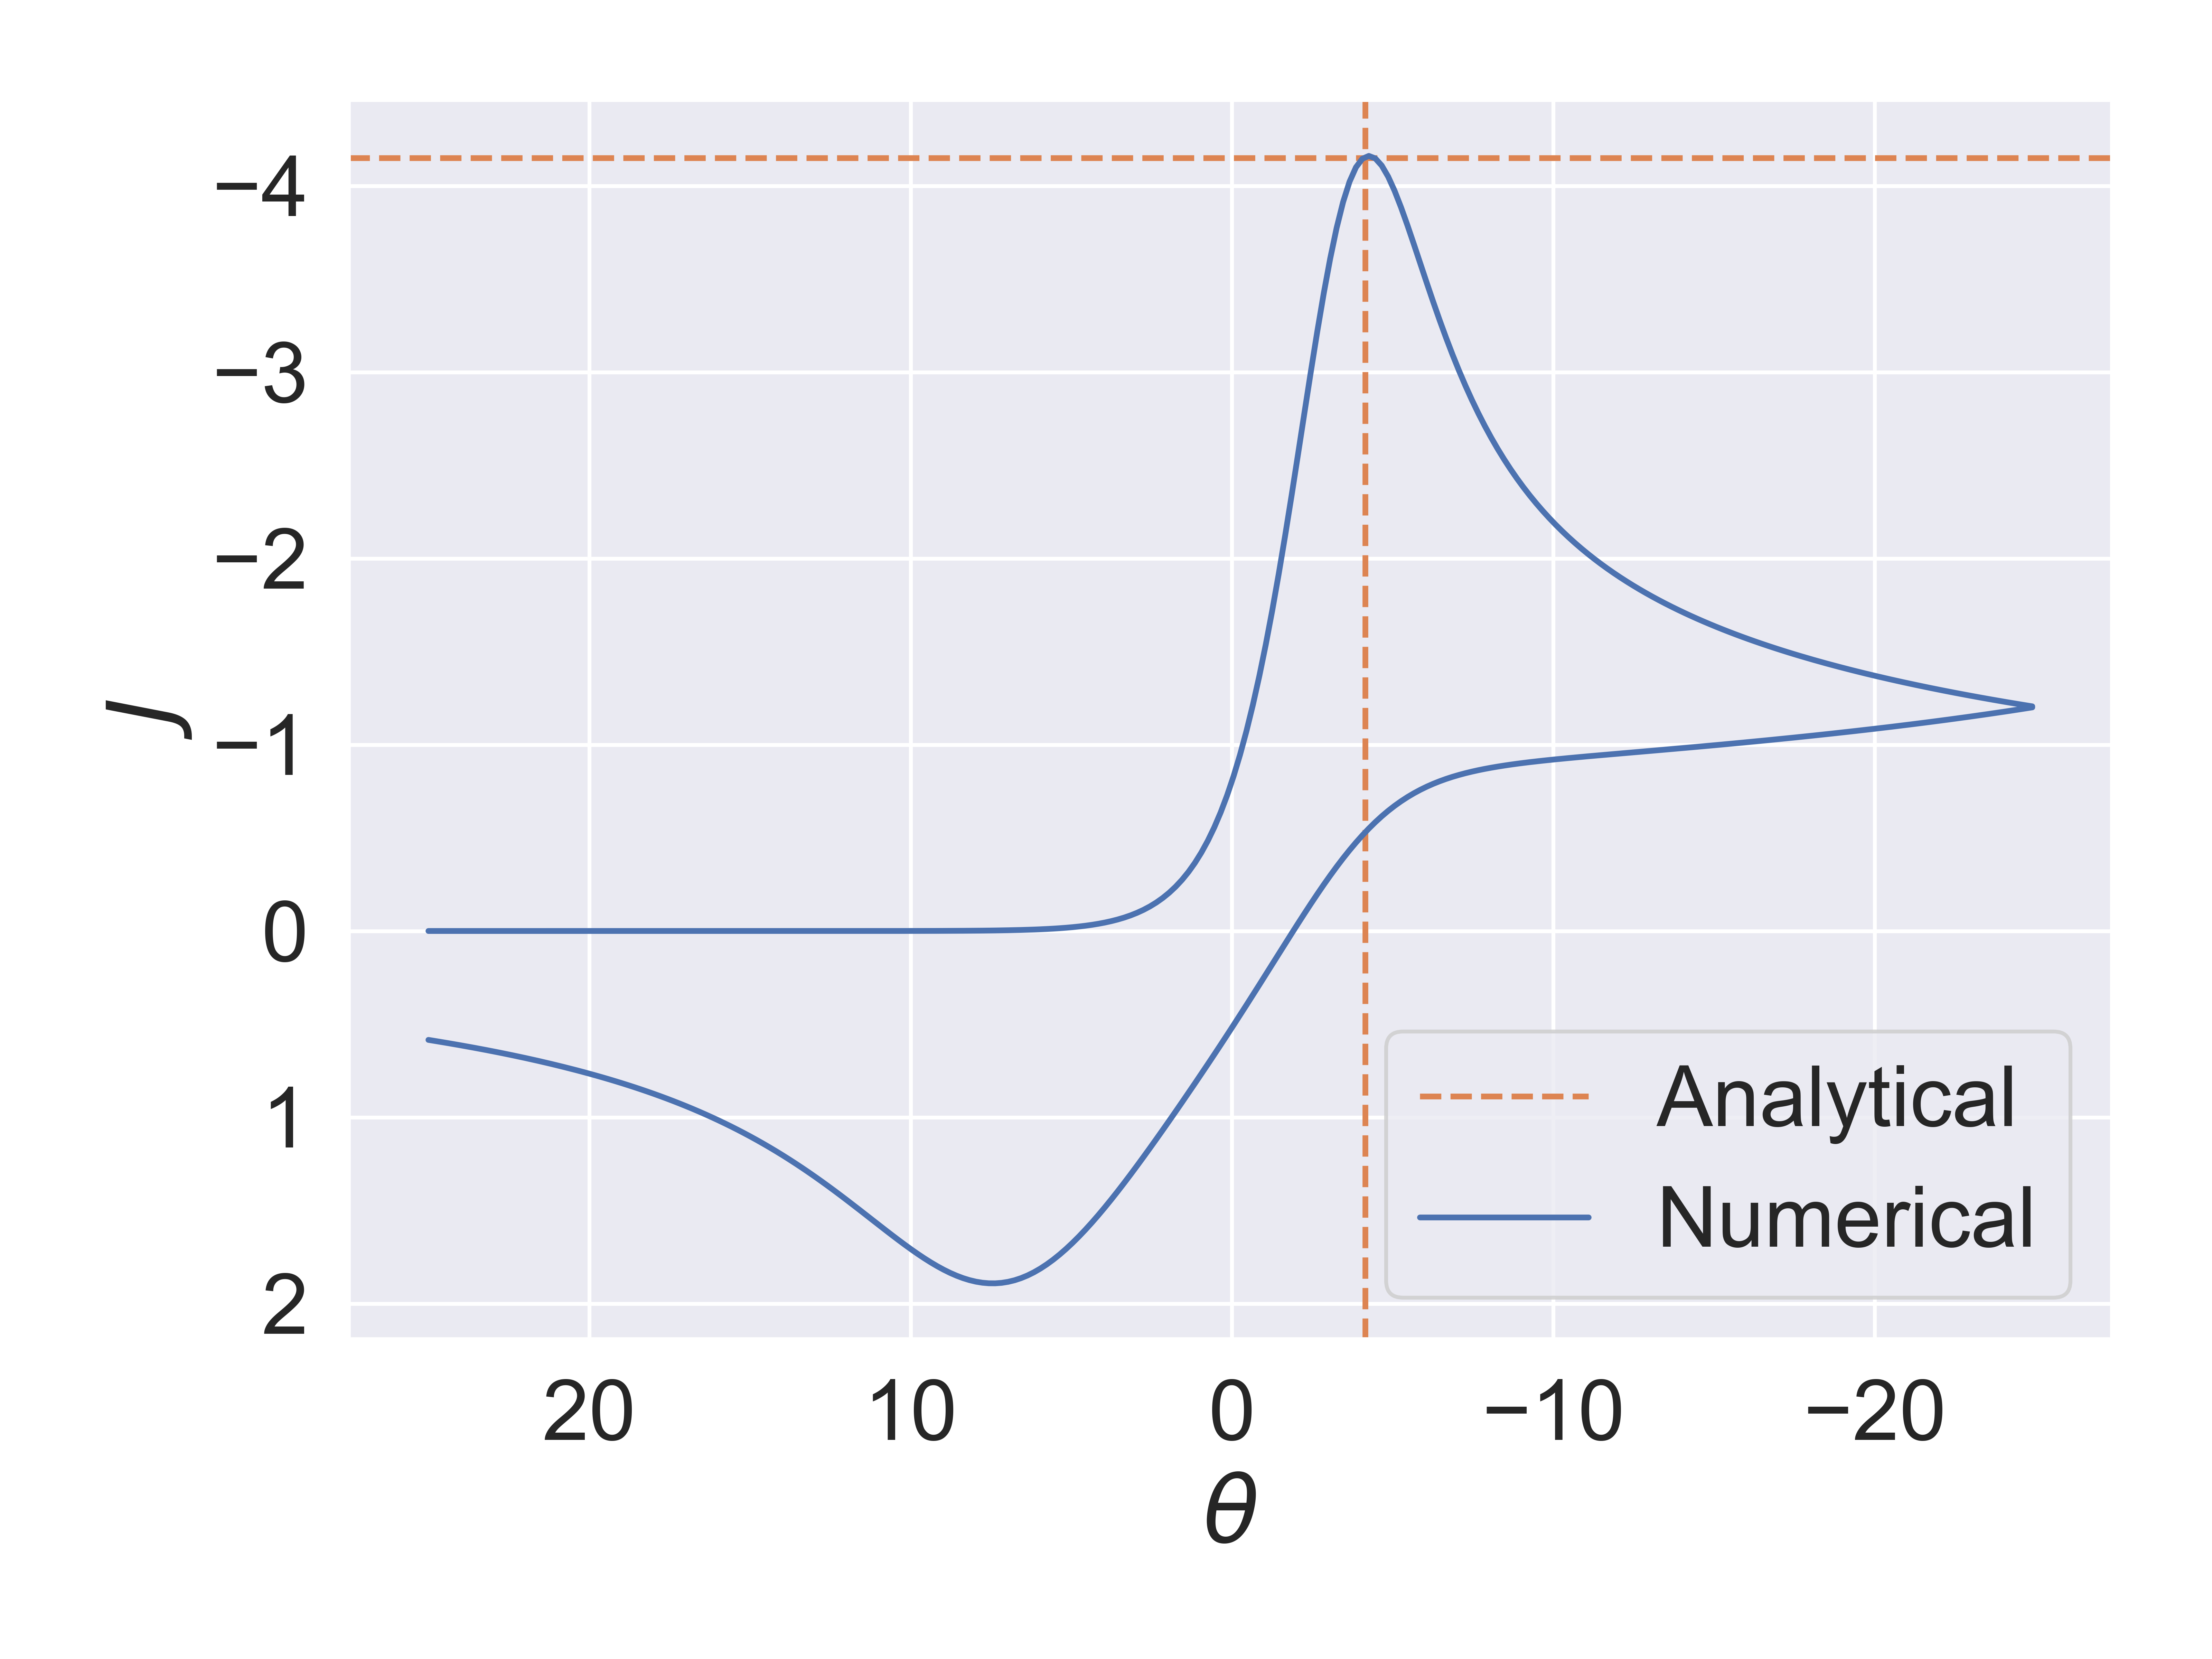
\includegraphics[width=0.8\textwidth]{figures/3-analytical.png}
  \caption[Verification of the forward solver against analytical
  peak-current expressions]{Verification of the forward solver with
    $\sigma = 1000$.
    Left: reversible limit ($K_0 = 1000, \ \alpha = 0.5$), compared with the
    Randles--\v{S}ev\v{c}\'{\i}k peak
    current~\cref{eq:randles-sevcik}.
    Right: irreversible limit ($K_0 = 1, \ \alpha = 0.5$), compared
  with~\cref{eq:irreversible-peak}.}
  \label{fig:electron-analytical}
\end{figure}

\section{Effect of Butler--Volmer Parameters}\label{sec:bv-effects}

The behaviour of the voltammogram depends on the \emph{kinetic regime},
which is characterised by the dimensionless ratio
\begin{equation}
  \Lambda = \frac{K_0}{\sqrt{\sigma}}.
  \label{eq:lambda_regime}
\end{equation}
When $\Lambda \gg 1$ the reaction is reversible and the electron transfer is
fast relative to diffusion; when $\Lambda \ll 1$ it is irreversible.
The intermediate quasi-reversible regime, where both kinetics and
diffusion influence the voltammogram, is the most informative for
parameter estimation.

\Cref{fig:elec-parameter-effect-quasi} illustrates the effect of each
Butler--Volmer parameter in the quasi-reversible regime. The transfer
coefficient $\alpha$ controls the asymmetry between cathodic and anodic
peaks; the rate constant $K_0$ governs peak sharpness and separation;
the formal potential $\theta_f$ translates the voltammogram along the
potential axis without altering peak shapes. Because changes in one
parameter can partially mimic changes in another -- for instance, a
smaller $K_0$ broadens and separates the peaks, which an adjustment in
$\theta_f$ can partially compensate -- the parameters are correlated,
and a point estimate alone may not capture the full uncertainty.

\begin{figure}[ht]
  \begin{center}
    
\includegraphics[width=0.95\textwidth]{figures/3-parameter-effect-quasi.png}
  \end{center}
  \caption[Effect of Butler--Volmer parameters on the quasi-reversible
  voltammogram]{Effect of each Butler--Volmer parameter on the dimensionless
    voltammogram for a quasi-reversible reaction ($K_0=20, \,
    \alpha=0.6, \, \sigma = 1000$). In each panel one
    parameter is varied while the others are held fixed. Left:
    varying~$\alpha$ changes the relative heights of the cathodic and
    anodic peaks. Centre: increasing~$K_0$ symmetrises and sharpens the
    voltammogram. Right: varying~$\theta_f$ translates the peaks along
  the potential axis.}
  \label{fig:elec-parameter-effect-quasi}
\end{figure}

The problem is compounded in the reversible regime.
\Cref{fig:alpha-k0-parameter-effect-rev} shows that at $K_0 = 200$
the voltammograms for $\alpha = 0.3, \, 0.5, \, 0.7$ are nearly
indistinguishable, and similarly for $K_0 = 200, \, 500, \, 1000$.
The combination of parameter correlations in the quasi-reversible
regime and negligible impact in the reversible regime motivates a
probabilistic treatment that can quantify these uncertainties and
reveal the correlation structure. We develop this in the next chapter.
\begin{figure}[ht]
  \begin{center}
    \includegraphics[width=0.8\textwidth]{figures/3-alpha-K0-effect-reversible.png}
  \end{center}
  \caption[Negligible impact of the transfer coefficient and rate
  constant in the reversible regime]{Left: effect of $\alpha$ in the
    reversible regime
    ($K_0 = 200$); the three curves are nearly indistinguishable.
    Right: effect of $K_0$ for values well into the reversible regime;
  again the voltammograms overlap.}
  \label{fig:alpha-k0-parameter-effect-rev}
\end{figure}

\chapter{Bayesian Approach to the Inverse Problem}\label{ch:bayesian}

In general, data obtained from a voltammetry experiment will be noisy and
subject to experimental error. Further, as discussed in
\cref{sec:bv-effects}, there may be multiple configurations of parameters
that produce similar current waveforms, and certain parameters may have
negligible influence on the voltammogram in particular kinetic regimes.
This makes the problem of recovering the parameters of the experiment
given the observed data --- the \emph{inverse problem} ---
\emph{ill-posed}: a unique, stable solution may not exist. For this
reason, we take a Bayesian approach and seek probability distributions
over the parameters rather than point estimates. This framework naturally
quantifies the uncertainty in each parameter and reveals correlations
between them.

\section{Noise Model}\label{sec:noise-model}

%TODO: Define the noise level to be based on the peak current

We model the observed dimensionless flux data as the output of the
forward map~$\mathcal{P}$ corrupted by additive Gaussian noise. Let
$\mathbf{y} = (y_1, \ldots, y_N)$ denote the $N$ flux measurements
recorded at discrete time levels. We assume
\begin{equation}
  y_i = \mathcal{P}(\phi)_i + \varepsilon_i,
  \qquad \varepsilon_i \overset{\mathrm{iid}}{\sim}
  \mathcal{N}(0,\, \varsigma^2),
  \label{eq:noise-model}
\end{equation}
where $\mathcal{P}(\phi)_i$ is the $i$th component of the simulated flux
trajectory for parameter vector~$\phi = (\alpha,\, K_0,\, \theta_f)$,
and $\varsigma^2$ is the variance of the measurement noise, which we
treat as a known constant throughout. We use $\varsigma$ rather
than~$\sigma$ to avoid confusion with the dimensionless scan rate defined
in the previous chapters.

An example of such noisy data is shown in \cref{fig:noisy-samples}.

\begin{figure}[ht]
  \begin{center}
    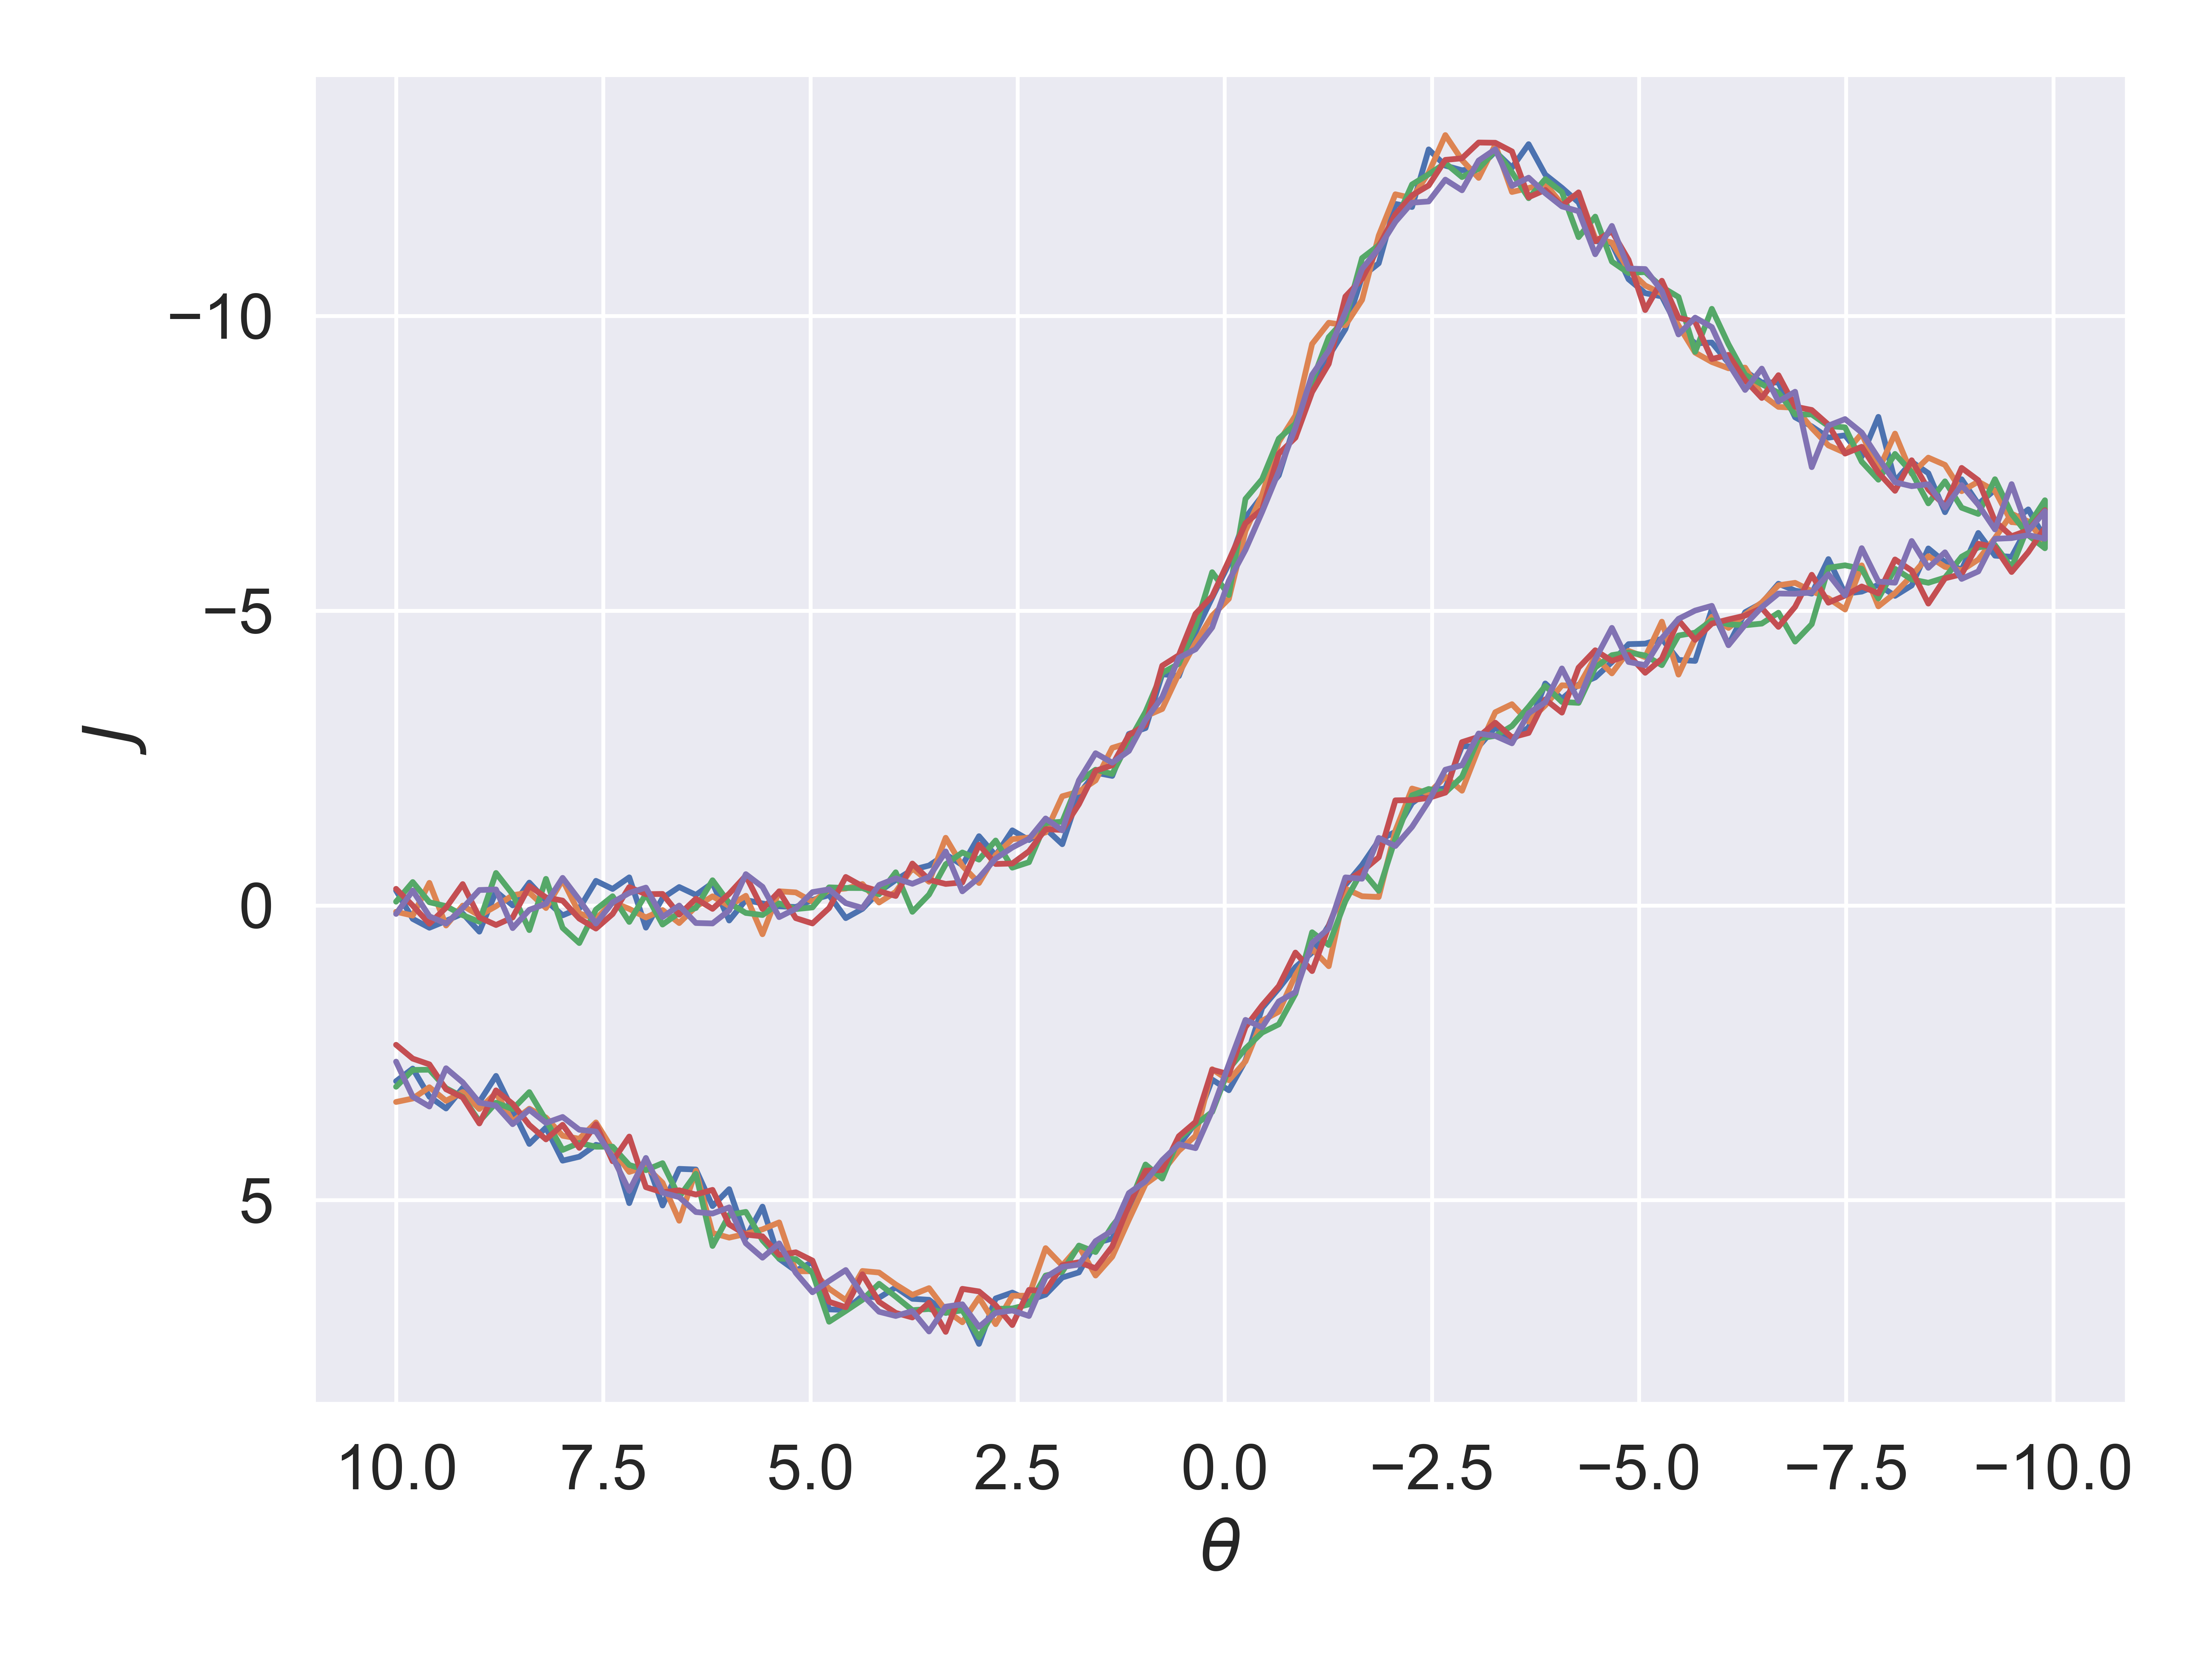
\includegraphics[width=0.6\textwidth]{figures/4-noisy-data.png}
  \end{center}
  \caption{Synthetic voltammogram data generated by evaluating the forward
    map~$\mathcal{P}$ with dimensionless scan rate $\sigma = 1000$ over
    the potential window $\theta_i = 10$ to $\theta_v = -10$, then
    adding i.i.d.\ Gaussian noise with $\varsigma = 0.25$. The noisy
    observations (points) are the data~$\mathbf{y}$ from which the
  Butler--Volmer parameters are to be inferred.}
  \label{fig:noisy-samples}
\end{figure}

\section{Posterior Distribution}\label{sec:posterior}

Bayes' theorem relates the posterior distribution of the parameters given
the data to the likelihood and prior:
\begin{equation}
  p(\phi \mid \mathbf{y})
  = \frac{L(\mathbf{y} \mid \phi)\, \pi(\phi)}{p(\mathbf{y})},
  \label{eq:bayes}
\end{equation}
where $L(\mathbf{y} \mid \phi)$ is the likelihood,
$\pi(\phi)$ is the prior distribution, and
$p(\mathbf{y}) = \int L(\mathbf{y} \mid \phi)\, \pi(\phi)\, d\phi$
is the marginal likelihood (or evidence), which serves as a normalising
constant independent of~$\phi$.

\subsection{Prior}

We adopt an uninformative prior: a uniform distribution over physically
reasonable bounds for each parameter,
\begin{equation}
  \pi(\phi) \propto 1 \qquad \text{for } \phi \in \Phi,
  \label{eq:prior}
\end{equation}
where $\Phi \subset \mathbb{R}^3$ is a bounded region encoding
constraints such as $\alpha \in (0,1)$ and $K_0 > 0$. Within~$\Phi$ the
prior is constant and therefore does not favour any particular parameter
combination. Consequently, the posterior is proportional to the
likelihood:
\begin{equation}
  p(\phi \mid \mathbf{y}) \propto L(\mathbf{y} \mid \phi).
  \label{eq:posterior-proportional}
\end{equation}

\subsection{Likelihood}

Under the noise model~\cref{eq:noise-model}, the observations are
conditionally independent given~$\phi$, and the likelihood takes the
form
\begin{equation}
  L(\mathbf{y} \mid \phi)
  = \prod_{i=1}^{N} \frac{1}{\sqrt{2\pi\varsigma^2}}
  \exp\!\left(
    -\frac{\big(y_i - \mathcal{P}(\phi)_i\big)^2}{2\varsigma^2}
  \right).
  \label{eq:likelihood}
\end{equation}
In practice we work with the log-likelihood. Taking the logarithm
of~\cref{eq:likelihood} gives
\begin{equation}
  \log L(\mathbf{y} \mid \phi)
  = -\frac{N}{2}\log(2\pi\varsigma^2)
  - \frac{1}{2\varsigma^2}
  \sum_{i=1}^{N}\big(y_i - \mathcal{P}(\phi)_i\big)^2.
  \label{eq:full-log-likelihood}
\end{equation}
Since $\varsigma$ is treated as known, the first term is a constant that
does not depend on~$\phi$ and can be dropped when comparing likelihoods
at different parameter values. We therefore define the log-likelihood
function used in all subsequent computations as
\begin{equation}
  \ell(\phi)
  = -\frac{1}{2\varsigma^2}
  \sum_{i=1}^{N}\big(y_i - \mathcal{P}(\phi)_i\big)^2.
  \label{eq:log-likelihood}
\end{equation}

\section{Markov Chain Monte Carlo}\label{sec:mcmc}

The posterior distribution~\cref{eq:posterior-proportional} is known only
up to a normalising constant, and the integral defining that constant is
generally intractable for non-trivial forward maps. \emph{Markov chain
Monte Carlo} (MCMC) provides a numerical approach: rather than evaluating
the posterior everywhere, we construct a Markov chain whose stationary
distribution is the posterior and use the samples generated by the chain
to approximate expectations and marginal distributions.

\subsection{Markov Chain}

An MCMC method produces a sequence of parameter vectors
\begin{equation}
  \big\{\phi^{(0)},\, \phi^{(1)},\, \ldots,\, \phi^{(T)}\big\}
  \subseteq \Phi,
\end{equation}
where each $\phi^{(t+1)}$ depends only on the current
state~$\phi^{(t)}$ (the Markov property). Under regularity conditions ---
in particular, that the chain is irreducible and aperiodic --- the
ergodic theorem guarantees that the empirical distribution of the samples
converges to the target posterior as $T \to \infty$.

\subsection{Proposal Distribution}

At each step the chain generates a \emph{candidate} parameter vector from
a \emph{proposal distribution} $q(\cdot \mid \phi^{(t)})$:
\begin{equation}
  \phi_{\mathrm{cand}} \sim q(\cdot \mid \phi^{(t)}).
\end{equation}
The proposal distribution is a design choice that determines how the
chain explores the parameter space. Its form need not match the posterior,
but the efficiency of the sampler depends heavily on how well the
proposals reflect the local geometry of the target distribution.

\subsection{Acceptance Criterion}

Whether the chain moves to the candidate is determined by the
\emph{Metropolis--Hastings acceptance probability}~\cite{hastings1970monte}:
\begin{equation}
  r = \min\!\left\{
    \frac{p(\phi_{\mathrm{cand}} \mid \mathbf{y})\;
    q(\phi^{(t)} \mid \phi_{\mathrm{cand}})}
    {p(\phi^{(t)} \mid \mathbf{y})\;
    q(\phi_{\mathrm{cand}} \mid \phi^{(t)})},\; 1
  \right\}.
  \label{eq:mh-acceptance}
\end{equation}
A uniform random number $u \sim \mathrm{Uniform}(0,1)$ is drawn: if
$u < r$ the candidate is accepted and $\phi^{(t+1)} =
\phi_{\mathrm{cand}}$; otherwise the chain remains at
$\phi^{(t+1)} = \phi^{(t)}$. The ratio in~\cref{eq:mh-acceptance}
involves the posterior only through ratios, so the unknown normalising
constant cancels -- this is the key property that makes MCMC practical.

\section{Random Walk Metropolis--Hastings}\label{sec:rwmh}

The \emph{random walk Metropolis--Hastings} (RWMH) algorithm is a
particular instance of the Metropolis--Hastings framework in which the
proposal distribution is a symmetric Gaussian centred at the current
state:
\begin{equation}
  q(\phi_{\mathrm{cand}} \mid \phi^{(t)})
  = \mathcal{N}(\phi^{(t)},\, \Sigma),
  \label{eq:rwmh-proposal}
\end{equation}
where $\Sigma \in \mathbb{R}^{3 \times 3}$ is a positive-definite
covariance matrix that controls the size and orientation of the proposed
steps. Since the Gaussian density is symmetric ---
$q(\phi_{\mathrm{cand}} \mid \phi^{(t)}) = q(\phi^{(t)} \mid
\phi_{\mathrm{cand}})$ --- the proposal ratio
in~\cref{eq:mh-acceptance} is unity, and the acceptance probability
simplifies to
\begin{equation}
  r = \min\!\left\{
    \frac{p(\phi_{\mathrm{cand}} \mid \mathbf{y})}
    {p(\phi^{(t)} \mid \mathbf{y})},\; 1
  \right\}
  = \min\!\left\{
    \exp\!\big(\ell(\phi_{\mathrm{cand}}) - \ell(\phi^{(t)})\big),\; 1
  \right\},
  \label{eq:rwmh-acceptance}
\end{equation}
where the second equality uses~\cref{eq:posterior-proportional} and the
definition of the log-likelihood~\cref{eq:log-likelihood}. In practice,
we compute $\ell(\phi_{\mathrm{cand}}) - \ell(\phi^{(t)})$ directly to
avoid numerical overflow.

The choice of the proposal covariance~$\Sigma$ is critical to the
efficiency of the sampler. If the steps are too small the chain explores
the parameter space slowly and successive samples are highly correlated;
if the steps are too large most proposals fall in regions of low
posterior density and are rejected. A common heuristic is to
tune~$\Sigma$ to achieve an acceptance rate of
approximately $23\%$~\cite{gelman1997weak}, which is asymptotically
optimal for Gaussian targets in high dimensions.

\subsection{Sampling Results}\label{sec:sampling-results}

We apply the RWMH algorithm to synthetic data generated from the forward
map with known true parameters and additive Gaussian noise with
$\varsigma = 0.25$. \Cref{fig:rwmh-hist} shows the marginal posterior
histograms for each parameter. All three marginals concentrate around the
true parameter values, confirming that the sampler recovers the correct
region of the parameter space. The marginal for~$K_0$ and~$\theta_f$ are
sharply peaked, indicating that the data is informative for these
parameters; the marginal for~$\alpha$ is broader, consistent with the
weaker sensitivity discussed in \cref{sec:bv-effects}.

\begin{figure}[ht]
  \centering
  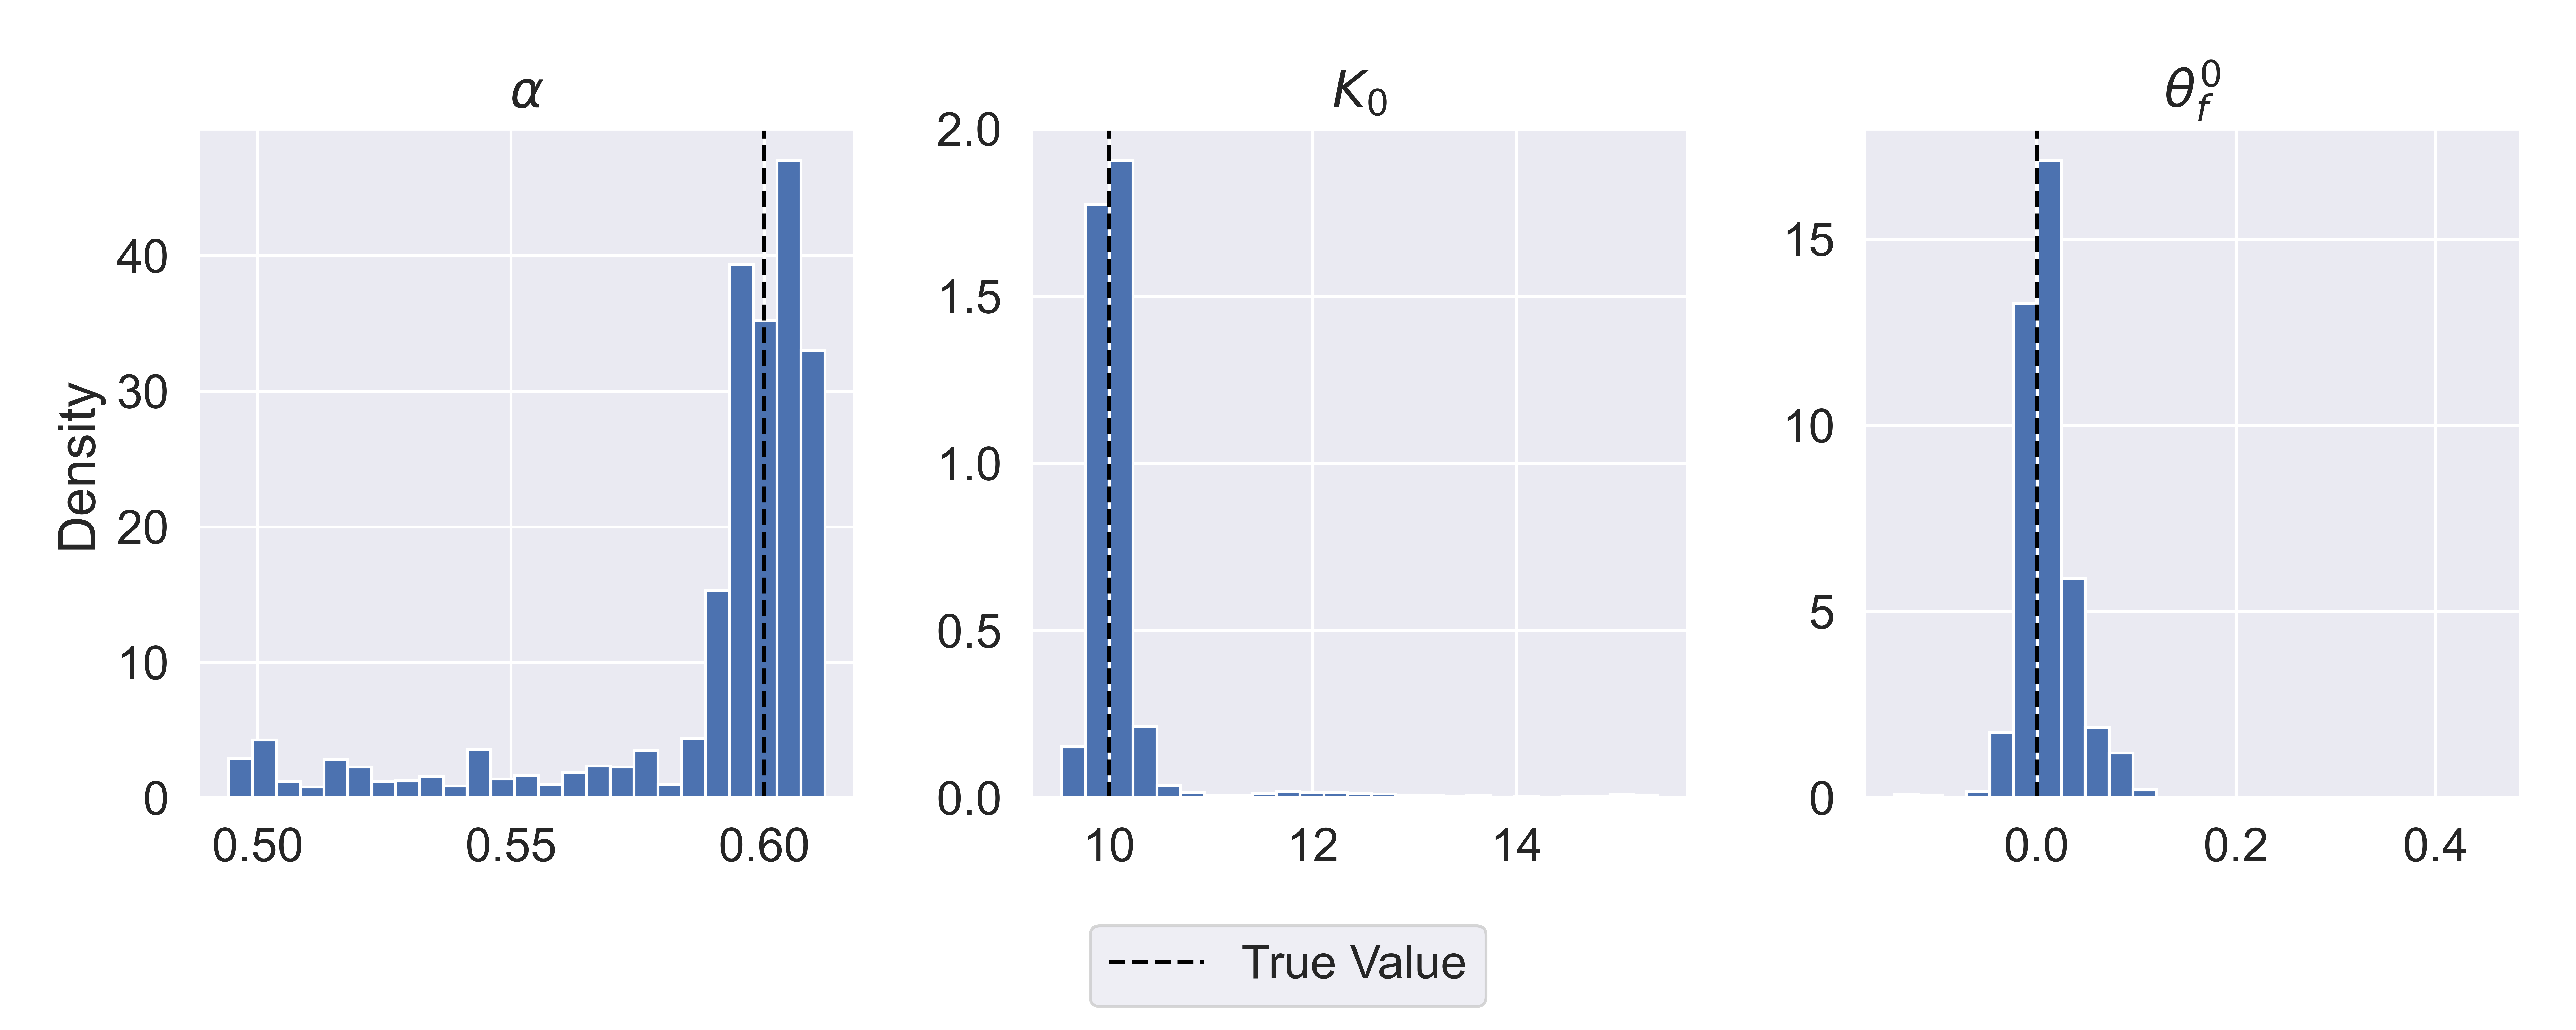
\includegraphics[width=0.95\textwidth]{figures/4-rwmh-hist.png}
  \caption{Marginal posterior histograms for the three Butler--Volmer
    parameters obtained by RWMH sampling on synthetic data with noise
    level $\varsigma = 0.25$. Dashed lines indicate the true parameter
    values used to generate the data. The posteriors for~$K_0$
    and~$\theta_f$ are tightly concentrated around the true values,
    while the marginal for~$\alpha$ is broader, reflecting its weaker
  influence on the voltammogram at this kinetic regime.}
  \label{fig:rwmh-hist}
\end{figure}

However, the histograms also exhibit extended tails, particularly
for~$\alpha$. The origin of these tails is visible in
\cref{fig:rwmh-burn-in}, which shows the $(\alpha, K_0)$ projection of
the chain coloured by sample index. The chain was initialised far from
the high-density region and spends a substantial number of iterations
traversing a low-probability ridge before settling near the true values.
The standard practice in MCMC is to discard these initial samples as
\emph{burn-in} and retain only the remainder as approximate draws from
the posterior. In principle this is straightforward; in our setting,
however, each likelihood evaluation requires a full run of the forward
map~$\mathcal{P}$, which involves solving the tridiagonal system at every
timestep. The cost of generating each proposal is therefore non-trivial,
and discarding a large burn-in period represents a significant waste of
computational effort.

\begin{figure}[ht]
  \centering
  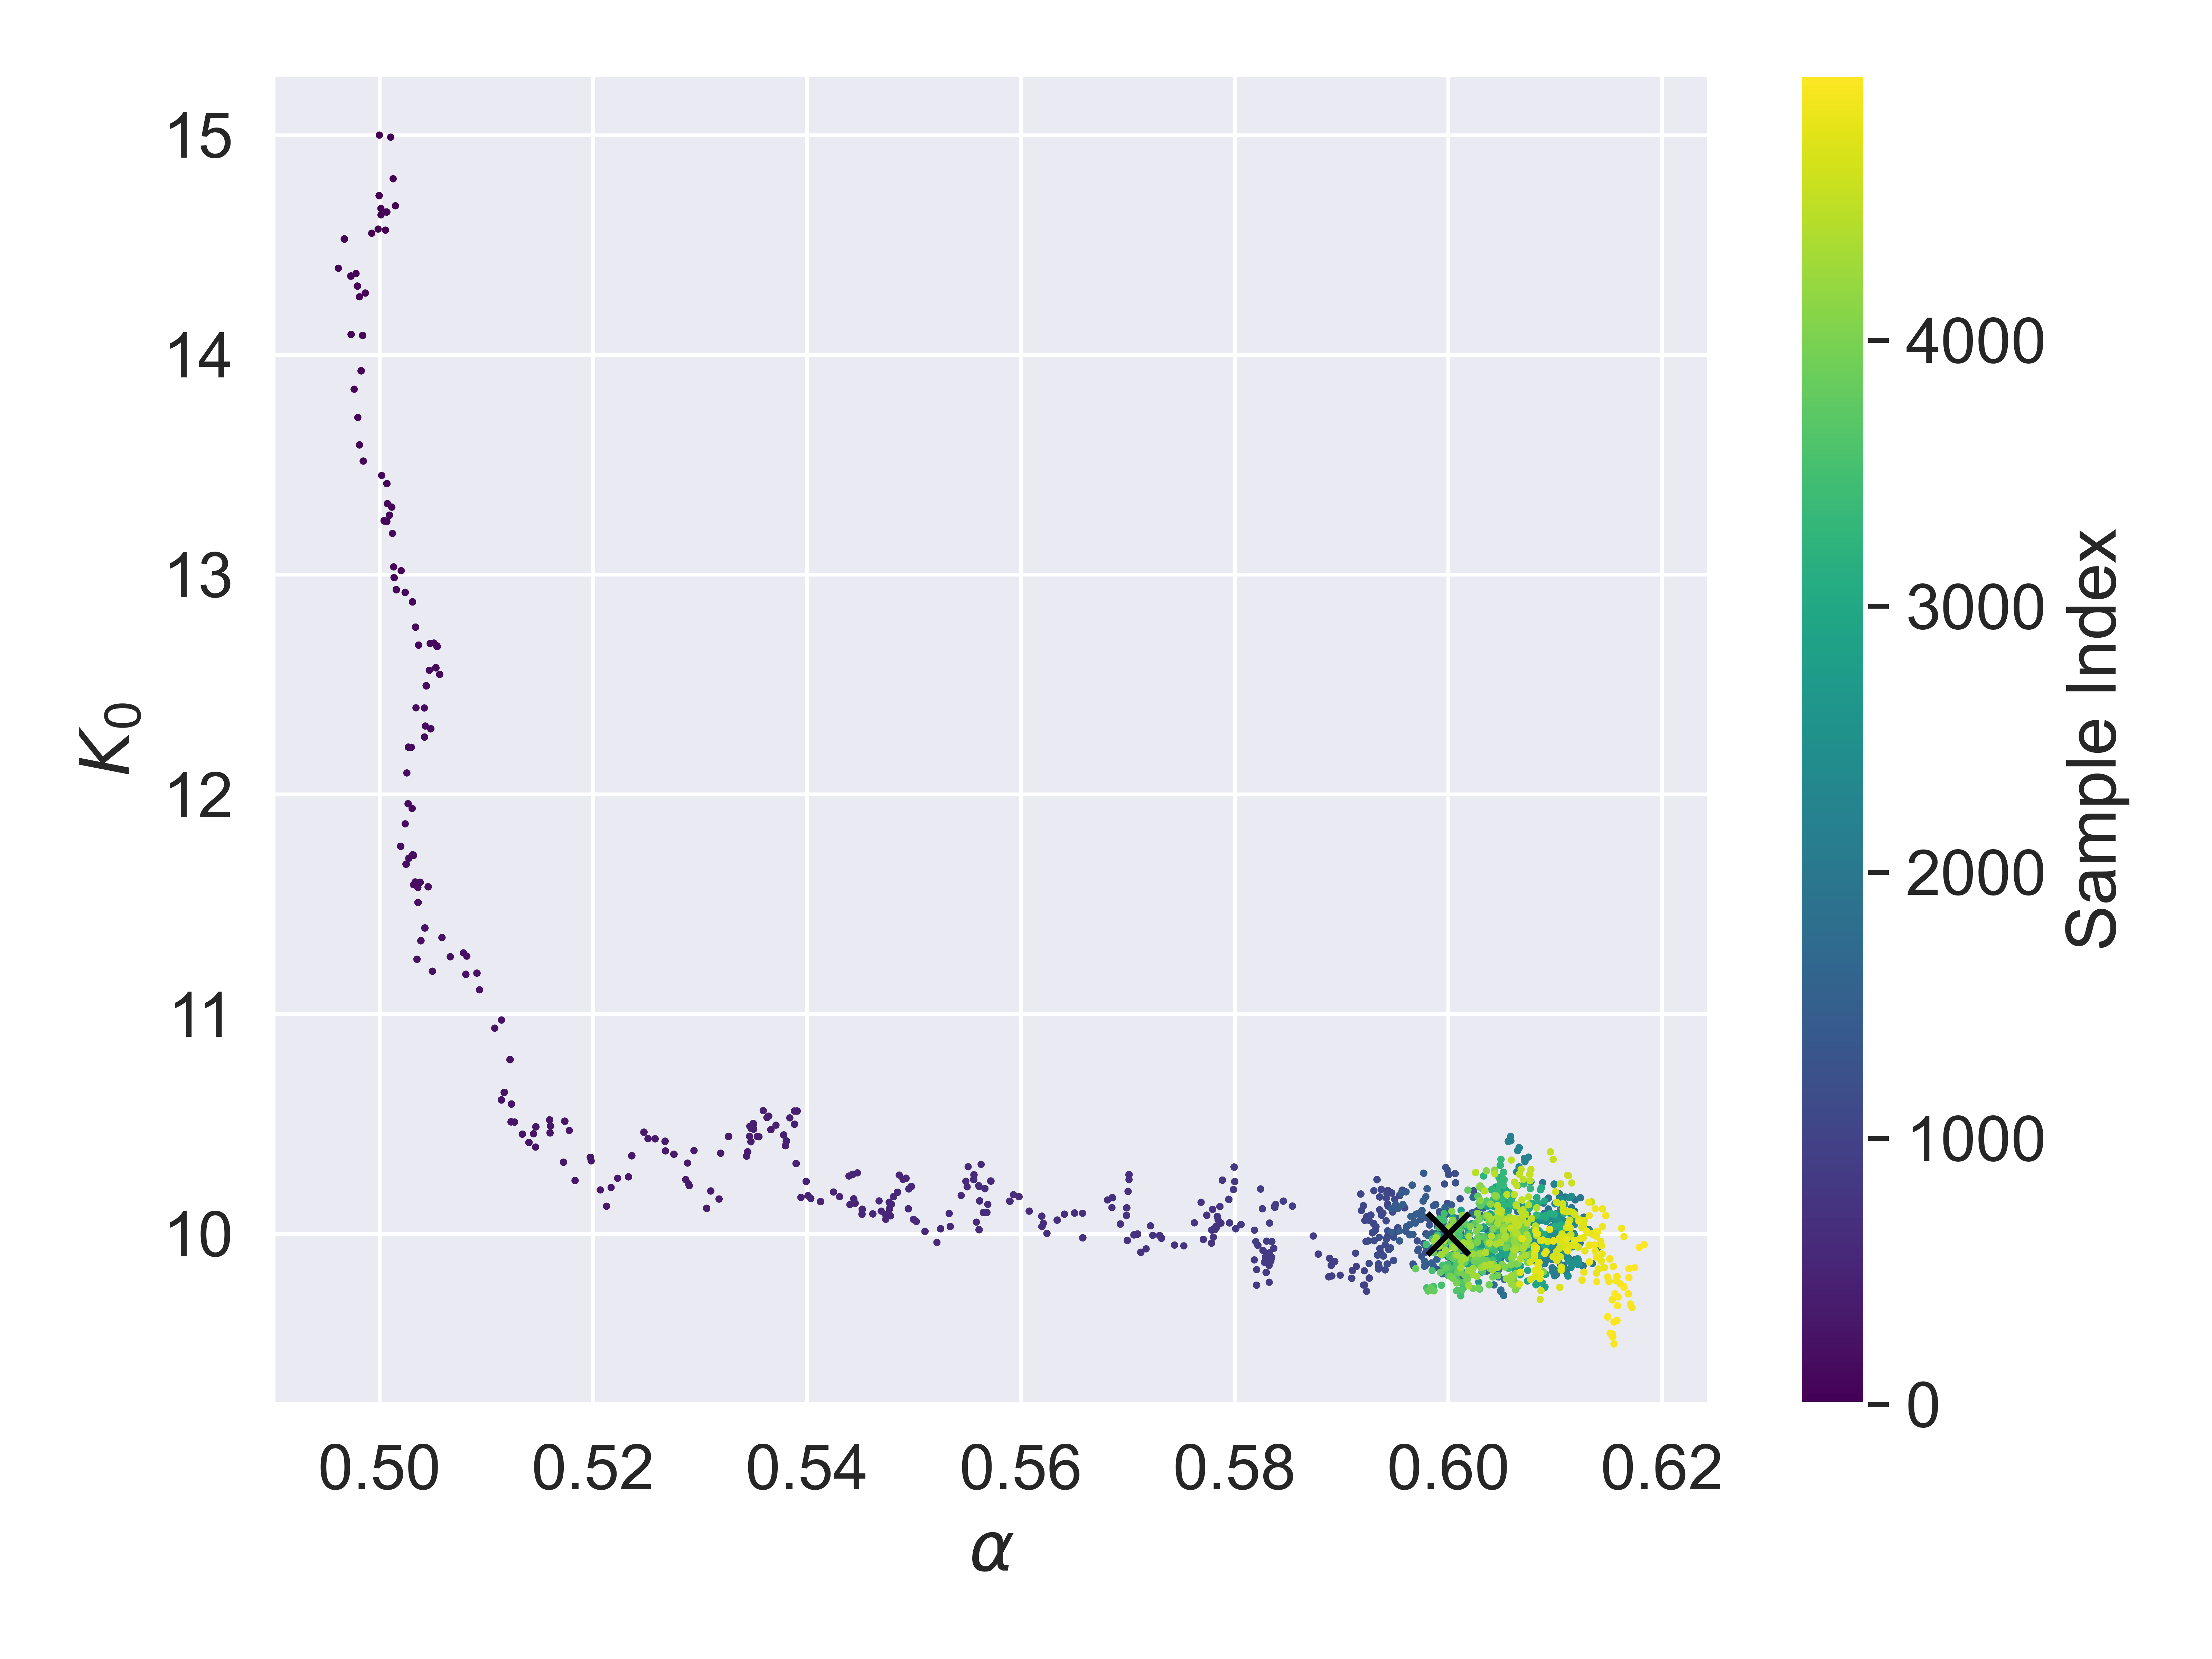
\includegraphics[width=0.8\textwidth]{figures/4-rwmh-scatter.png}
  \caption{Scatter plot of the RWMH chain projected onto the
    $(\alpha,\, K_0)$ plane. Points are coloured by sample index: early
    samples (dark) show the chain traversing a low-density region far
    from the true parameters (black cross), while later samples (light)
    concentrate near the posterior mode. The extended transient
    illustrates the cost of burn-in when each likelihood evaluation
  requires a full forward solve.}
  \label{fig:rwmh-burn-in}
\end{figure}

A more efficient strategy would be to first locate the high-density
region of the posterior --- effectively maximising the likelihood --- and
then initialise the Markov chain there, so that all samples contribute to
the posterior approximation from the outset. Gradient-based optimisation
methods are well suited to this task, as they exploit the local slope of
the likelihood surface to move rapidly toward the mode. More ambitiously,
gradient information can be incorporated into the MCMC proposal itself,
yielding samplers that explore the posterior far more efficiently than the
random walk. Both of these ideas require the ability to differentiate the
log-likelihood with respect to the parameters, which in turn requires
differentiating through the forward map~$\mathcal{P}$. We develop this
capability in the following chapter.

\chapter{Differentiating Through the Forward Solver}\label{ch:adjoint}

Computing the gradient $\nabla_\phi \ell$ of the
log-likelihood~\cref{eq:log-likelihood} requires differentiating through
the forward map~$\mathcal{P}$, which involves solving a sequence of
tridiagonal linear systems. In this chapter we derive an efficient adjoint
method for this computation, demonstrate its value through gradient-based
optimisation, and compare against a gradient-free alternative.

\section{Discretise Then Optimise}\label{sec:disc-then-opt}

There are two strategies for differentiating through a numerical solver.
The \emph{optimise then discretise} approach derives continuous adjoint
equations and then discretises them; the \emph{discretise then optimise}
approach differentiates the discrete computation directly. We adopt the
latter, which yields the exact gradient of the quantity evaluated in code
and avoids consistency errors between the forward and adjoint
discretisations~\cite{kidger2021neural}.

\section{Reverse-Mode AD and the Cost of Na\"ive Taping}%
\label{sec:reverse-ad}

Since $\ell$ is scalar-valued, reverse-mode automatic differentiation
(AD) computes the full gradient in a single backward pass regardless of
the number of parameters. Reverse-mode AD decomposes the computation into
a sequence of \emph{vector--Jacobian products} (VJPs): if the forward
computation is $f = f_L \circ \cdots \circ f_1$, the chain rule gives
\begin{equation}
  \frac{\partial f}{\partial \phi}
  = J_{f_L}\, J_{f_{L-1}} \cdots J_{f_1},
  \label{eq:chain-rule}
\end{equation}
which reverse mode evaluates from left to right, multiplying the adjoint
(cotangent) vector by each Jacobian in turn without forming the
intermediate matrices explicitly. The dominant primitives in
$\mathcal{P}$ are the $m$ tridiagonal solves, so the central question is
how to implement the VJP of a single solve $Ax = b$.

A generic AD framework will tape every intermediate scalar of the Thomas
algorithm -- elimination multipliers, modified diagonals, partial sums
-- and replay them in reverse. Since the tape must be retained across
all $m$ timesteps, the total memory scales as $O(mn)$ with a large
per-timestep constant, and the overhead of maintaining and traversing
the tape degrades runtime even when memory is not the binding constraint.

\section{Adjoint of the Tridiagonal Solve}\label{sec:adjoint-solve}

We avoid taping by exploiting the structure of the linear solve.
Suppose the forward pass solves $Ax = b$ and the backward pass receives
the adjoint $\bar{x} = \partial \ell / \partial x$. The adjoint with
respect to $b$ is
\begin{equation}
  \bar{b}
  = \bar{x}^T \frac{\partial x}{\partial b}
  = \bar{x}^T A^{-1},
  \label{eq:adjoint-b}
\end{equation}
which is equivalent to solving the \emph{adjoint system}
\begin{equation}
  A^T \lambda = \bar{x}
  \label{eq:adjoint-system}
\end{equation}
and setting $\bar{b} = \lambda^T$. For the matrix adjoint, we
differentiate the identity $Ax = b$:
\begin{equation}
  dA\, x + A\, dx = db.
\end{equation}
Left-multiplying by $\lambda^T$ and using $\lambda^T A = \bar{x}^T$
gives $\lambda^T dA\, x + \bar{x}^T dx = \lambda^T db$. Since
$\bar{x}^T dx$ contributes to $\bar{b}$, the
adjoint with respect to $A$ is
\begin{equation}
  \bar{A} = -\lambda\, x^T,
  \label{eq:adjoint-A}
\end{equation}
where $\bar{A}_{ij} = -\lambda_i\, x_j$.

The key observation is that $A^T$ is also tridiagonal, so the adjoint
system~\cref{eq:adjoint-system} is solved by the Thomas algorithm at the
same $O(n)$ cost as the forward solve. Only the matrix $A$ diagonals and the
forward solution $x$ need to be cached per timestep -- four arrays of
length $n$, rather than the full tape of Thomas algorithm intermediates.

In practice we define a custom VJP rule in
JAX~\cite{jax2018github}: the forward pass solves $Ax = b$ and caches
$A$ and $x$; the backward pass solves $A^T \lambda = \bar{x}$ and
returns $\bar{b} = \lambda^T$ and $\bar{A} = -\lambda\, x^T$. No taping
of the Thomas algorithm's internal operations is required.

\subsection{Full Backward Pass}\label{sec:full-backward}

The custom VJP handles a single timestep. The full gradient
$\nabla_\phi \ell$ is assembled by walking backward through time levels
$k = m, m-1, \ldots, 1$. At each level the adjoint
system~\cref{eq:adjoint-system} is solved using the cached $A^k$
and~$x^k$, yielding $\lambda^k$ and the matrix adjoint
$\bar{A}^k = -\lambda^k (x^k)^T$. Only the first row of $A^k$ depends
on $\phi$ (through the Butler--Volmer coefficients $K_{\mathrm{red}}$
and $K_{\mathrm{ox}}$; the interior rows are parameter-independent), so
the contributions to $\nabla_\phi \ell$ come exclusively from $\bar{A}^k$
applied to the partial derivatives $\partial A^k_{0,\cdot} / \partial
\phi$, which are accumulated across timesteps. The result is the exact
gradient of the discrete log-likelihood at a cost of one adjoint solve
per timestep.

\section{Extension to Pentadiagonal Systems}\label{sec:pentadiagonal}

The adjoint generalises directly to pentadiagonal systems: the transpose
of a pentadiagonal matrix is again pentadiagonal, so the adjoint system
is solved at the same $O(n)$ cost per timestep. The saving over na\"ive
taping grows with bandwidth, since a pentadiagonal factorisation produces
more intermediates. We exploit this in
\cref{ch:heterogeneous,ch:adsorption}, where coupled multi-species
reactions lead to pentadiagonal structure.

\section{Optimisation Results}\label{sec:init-results}

We now use the adjoint gradient to locate the posterior mode before
sampling, eliminating the burn-in waste observed in
\cref{sec:sampling-results}. We compare the gradient-based ADAM
optimiser~\cite{kingma2014adam,deepmind2020jax} against
CMA-ES~\cite{hansen2001evolution,evosax2022github},
a gradient-free evolutionary strategy that adapts a population covariance
over generations. A single ADAM step (one forward and one adjoint solve)
costs approximately two forward-solve equivalents; one CMA-ES generation
costs $\lambda = 4 + \lfloor 3 \times \ln d\rfloor = 7$
\cite{hansen2001evolution}
forward solves. We equalise the total budget in forward-solve
equivalents so that both algorithms consume the same runtime.

\Cref{fig:electron-optim} shows the log-posterior density over the
course of optimisation at two noise levels ($\eta = 0.01$ and
$\eta = 0.02$), each run from $32$ initial conditions drawn using
Latin hypercube sampling centered at the true parameters. ADAM
reaches the high-density region in fewer
forward-solve equivalents and with lower variance across initialisations:
at $\eta = 0.02$, all $32$ runs are within $5\%$ of the modal
log-density by iteration $100$. Once ADAM reaches the mode it remains
stable, making it a suitable initialisation strategy for the MCMC
samplers. The difference between the performance of these
optimisation methods is not important in this problem -- we could use
CMA-ES to initialise the chains and obtain similar results -- but
this is not true when we increase the complexity of the problems. As
we will see in \cref{ch:heterogeneous,ch:adsorption}, the gradient
based optimisation becomes crucial to finding posterior modes efficiently.

\begin{figure}[ht]
  \begin{center}
    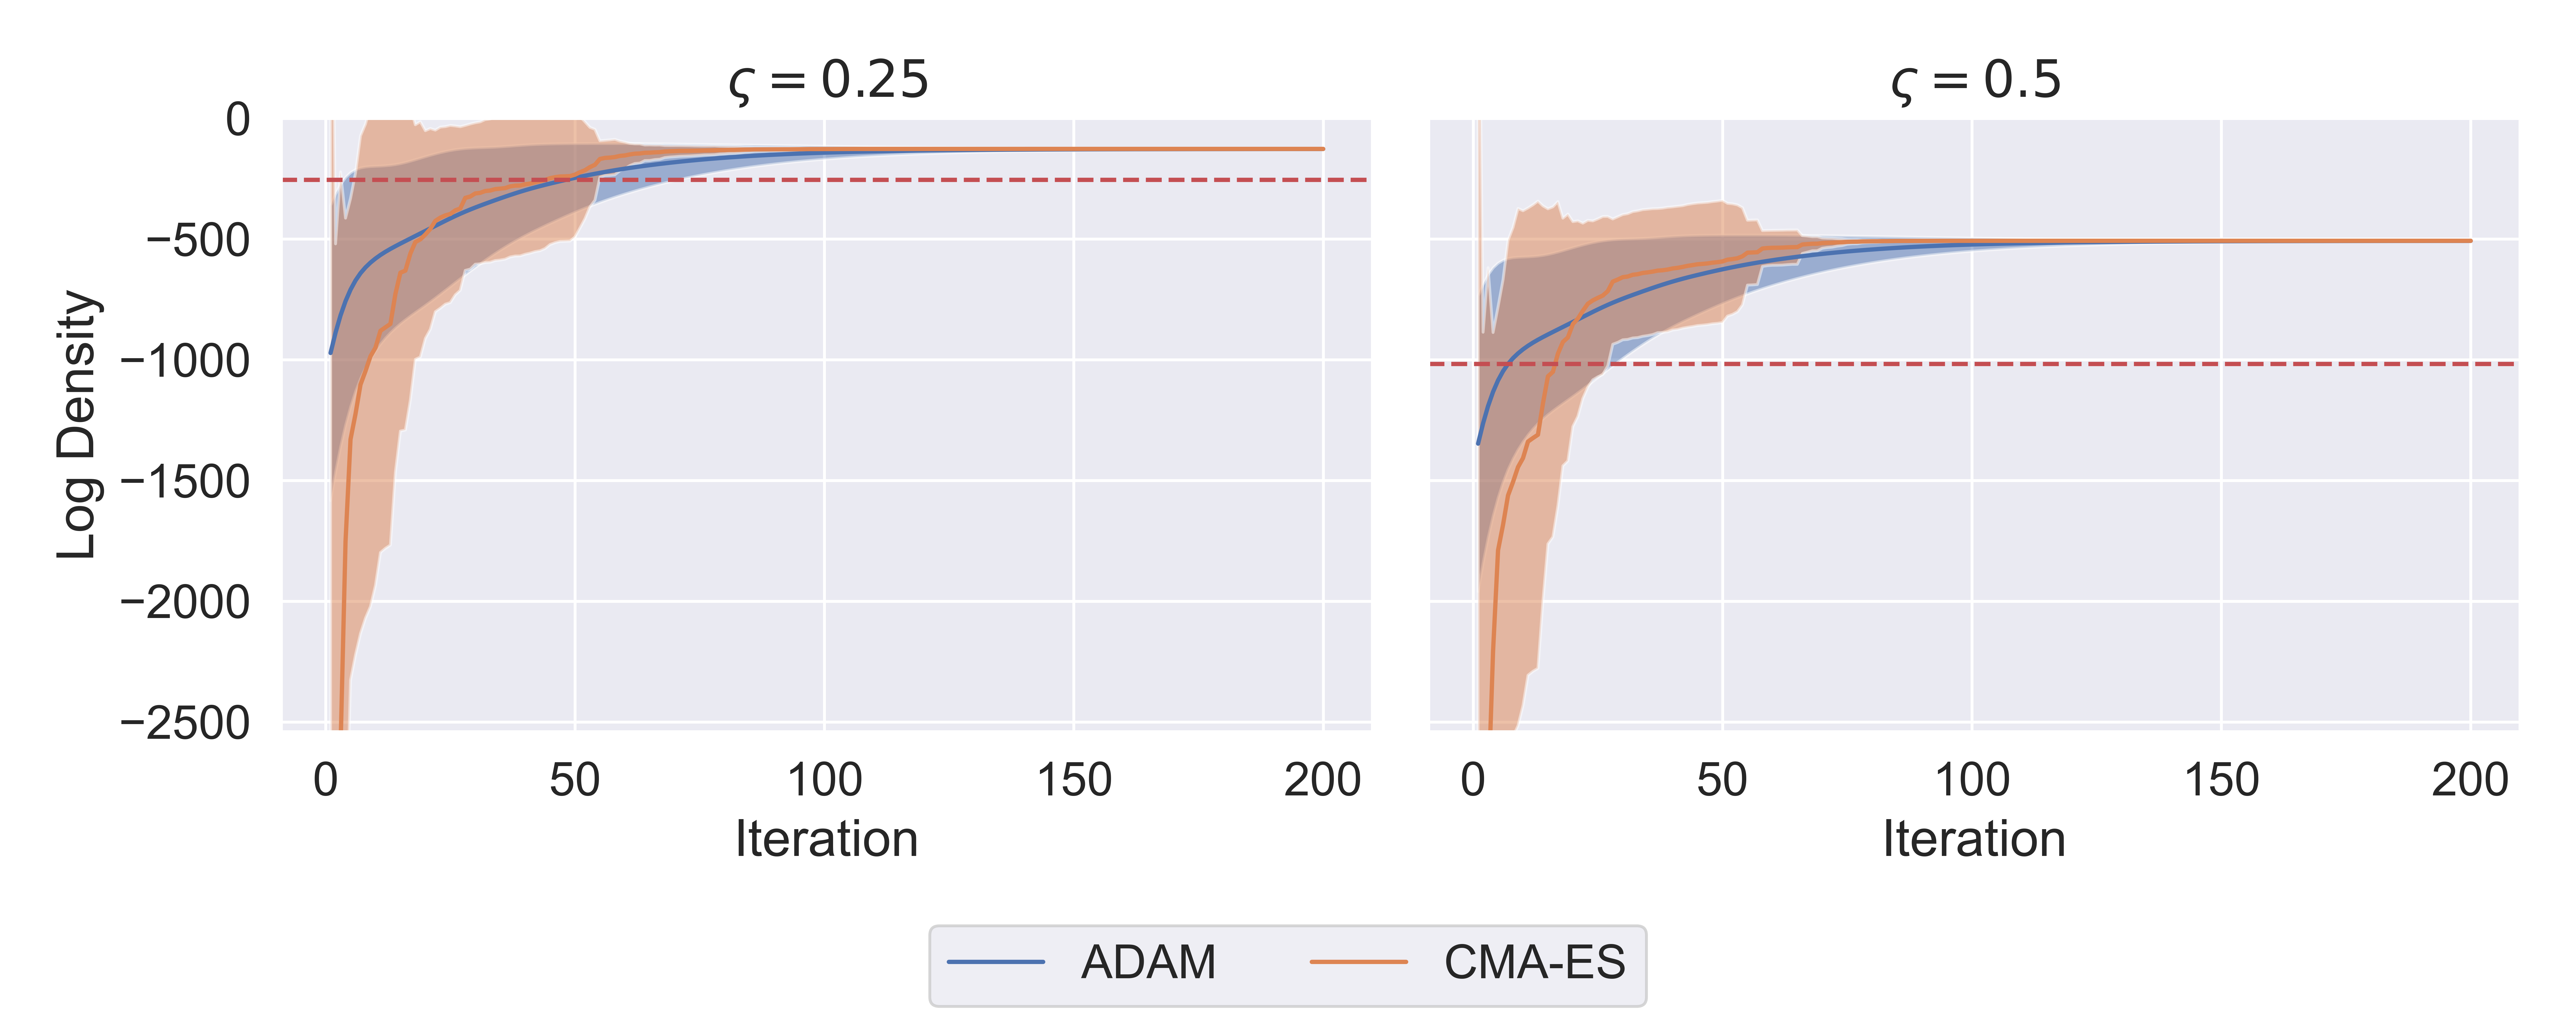
\includegraphics[width=0.95\textwidth]{figures/5-optim.png}
  \end{center}
  \caption[ADAM vs CMA-ES optimisation comparison]{Log-posterior density
    during optimisation for ADAM and CMA-ES (population size~$7$) at
    noise levels $\eta = 0.02$ and $\eta = 0.01$. Each algorithm is run
    from $32$~randomly drawn initial conditions; solid lines show the
    mean and shaded regions indicate $\pm 1$ standard deviation across
    runs. The black dashed line marks the two times the log-density
    evaluated at the true parameters~$\phi^*$ -- indicating high
    density regions. Both algorithms are given equal total
    computational budgets measured in forward-solve equivalents. 105
  steps for ADAM and 30 iterations for CMA-ES.}
  \label{fig:electron-optim}
\end{figure}

\chapter{Hamiltonian Monte Carlo}\label{ch:hmc}

The random walk Metropolis--Hastings algorithm explored in
\cref{ch:bayesian} generates proposals by perturbing the current state
with isotropic Gaussian noise. This strategy ignores the geometry of the
posterior: proposals are equally likely in every direction, regardless of
whether the posterior is steep or flat. Now that we have the ability to
differentiate through the forward map, we can exploit gradient information
to guide the sampler along the posterior surface. \emph{Hamiltonian Monte
Carlo} (HMC)~\cite{betancourt2018hamiltonian,neal2011mcmc} does precisely
this by borrowing the formalism of Hamiltonian dynamics to construct
proposals that are both distant from the current state and likely to be
accepted.

The physical intuition is as follows. We imagine the current position of
the Markov chain as a particle moving in the parameter space. At each
step, the particle is given a random kick (a momentum draw) and then
allowed to evolve under a Hamiltonian that couples its position to the
posterior. Because the dynamics conserve energy, the particle naturally
spends more time in regions of high posterior density and traces out
long-range, low-energy trajectories that would take a random walk many
steps to traverse.

\section{The Hamiltonian}\label{sec:hamiltonian}

Let $q \in \mathbb{R}^d$ denote the position (i.e.\ the parameter
vector~$\phi$; we use $q$ to follow the Hamiltonian mechanics convention)
and introduce an auxiliary momentum variable $p \in \mathbb{R}^d$. We
define the joint density of position and momentum through the canonical
distribution
\begin{equation}
  P(q, p) \propto \exp\!\big({-H(q, p)}\big),
  \label{eq:canonical-distribution}
\end{equation}
where $H(q, p)$ is the Hamiltonian. We decompose $H$ into a potential
energy~$U(q)$ and a kinetic energy~$K(p)$:
\begin{equation}
  H(q, p) = U(q) + K(p).
  \label{eq:hamiltonian-decomposition}
\end{equation}
This separation ensures that the joint density factorises as
$P(q, p) \propto \exp(-U(q))\,\exp(-K(p))$, so the position and momentum
are independent: marginalising over~$p$ recovers the target distribution
over~$q$ alone. We define the potential energy as the negative
log-posterior,
\begin{equation}
  U(q) = -\log p(q \mid \mathbf{y}) = -\ell(q) + \text{const},
  \label{eq:potential-energy}
\end{equation}
where the constant absorbs the normalising factor. Regions of high
posterior density correspond to low potential energy, so the particle
rolls into valleys at the posterior modes and must climb uphill to
escape. The kinetic energy is the quadratic form
\begin{equation}
  K(p) = \tfrac{1}{2}\, p^T M^{-1} p,
  \label{eq:kinetic-energy}
\end{equation}
where $M \in \mathbb{R}^{d \times d}$ is a symmetric positive-definite
\emph{mass matrix}. Under~\cref{eq:canonical-distribution} the momentum
is distributed as $p \sim \mathcal{N}(0, M)$. A well-chosen~$M$ that
approximates the posterior covariance preconditions the dynamics so that
the particle explores all directions at a similar rate.

\section{Leapfrog Integration and Metropolis
Correction}\label{sec:hmc-algorithm}

Hamilton's equations of motion for the
system~\cref{eq:hamiltonian-decomposition} are
\begin{equation}
  \frac{dq}{dt} = \frac{\partial H}{\partial p} = M^{-1}p,
  \qquad
  \frac{dp}{dt} = -\frac{\partial H}{\partial q} = -\nabla_q U(q).
  \label{eq:hamiltons-equations}
\end{equation}
The gradient $\nabla_q U(q) = -\nabla_q \ell(q)$ is computed via the
adjoint method described in \cref{ch:adjoint}. In practice these equations
are integrated numerically using the \emph{leapfrog} integrator, which is
symplectic and time-reversible. Given a step size~$\varepsilon$ and
$L$~integration steps, one leapfrog trajectory from $(q_0, p_0)$ proceeds
as:
\begin{equation}
  \begin{aligned}
    p_{i+1/2} &= p_i - \tfrac{\varepsilon}{2}\,\nabla_q U(q_i), \\
    q_{i+1}   &= q_i + \varepsilon\, M^{-1} p_{i+1/2}, \\
    p_{i+1}   &= p_{i+1/2}
    - \tfrac{\varepsilon}{2}\,\nabla_q U(q_{i+1}),
  \end{aligned}
  \label{eq:leapfrog}
\end{equation}
for $i = 0, 1, \ldots, L-1$. Each step requires one evaluation of
$\nabla_q U$, so a trajectory of $L$~steps costs $L$~gradient
evaluations, each involving a full forward and adjoint solve.

Because the leapfrog integrator introduces a discretisation error, the
Hamiltonian is not exactly conserved along the trajectory. To ensure
the chain targets the correct stationary distribution, a Metropolis
acceptance step is applied: the endpoint $(q^*, p^*)$ of the trajectory
is accepted with probability

\begin{equation}
  r = \min\!\big\{1,\;
  \exp\!\big(H(q, p) - H(q^*, p^*)\big)\big\}.
  \label{eq:hmc-acceptance}
\end{equation}

Since the integrator is symplectic, the energy error is typically small
and the acceptance rate is high even for proposals that are far from the
current state. The momentum is discarded after each accept/reject
decision; a fresh draw from $\mathcal{N}(0, M)$ at the start of each
iteration randomises the energy level and ensures the particle explores
the full posterior.

\section{The No-U-Turn Sampler}\label{sec:nuts}

The efficiency of HMC depends on the step size~$\varepsilon$ and
trajectory length~$L$. If $L$ is too small the sampler reverts to
near-random-walk behaviour; if $L$ is too large the trajectory doubles
back on itself, wasting gradient evaluations. The \emph{No-U-Turn
Sampler} (NUTS)~\cite{hoffman2014no} eliminates the need to specify~$L$
by doubling the trajectory in both directions until a U-turn criterion is
met. At each doubling the algorithm checks whether the endpoints of the
trajectory are moving apart; when they begin to converge the trajectory
is terminated and a sample is drawn uniformly from the valid states along
it. This adaptive scheme sets the trajectory length automatically at each
iteration, requiring only the step size~$\varepsilon$ and mass
matrix~$M$ to be specified.

\section{Parameter Transformations}\label{sec:transformations}

The leapfrog integrator applies a uniform step size~$\varepsilon$ in
every coordinate. If the parameters live on different scales or have
bounded support, the sampler performs poorly: it may step outside the
feasible region or waste steps on parameters whose natural scale is much
smaller than the step size. We address this by transforming the
Butler--Volmer parameters to an unconstrained space in which all
coordinates have comparable scale.

The transfer coefficient is constrained to the unit interval,
$\alpha \in (0,1)$; we apply the logit transform
\begin{equation}
  \tilde{\alpha} = \operatorname{logit}(\alpha)
  = \log\!\left(\frac{\alpha}{1 - \alpha}\right).
  \label{eq:logit-alpha}
\end{equation}
The dimensionless rate constant is constrained to be positive,
$K_0 > 0$; we apply the log transform
\begin{equation}
  \tilde{K}_0 = \log K_0.
  \label{eq:log-K0}
\end{equation}
The formal potential~$\theta_f$ is already unconstrained and requires no
transformation. The sampler operates in the transformed space
$\tilde{\phi} = (\tilde{\alpha},\, \tilde{K}_0,\, \theta_f)$, these
proposals are then transformed back into the dimensionless parameters
before being run through the solver. We tape these transformation to
ensure the correctness of the gradient updates.

\section{Inference Workflow}\label{sec:workflow}

We now describe the full inference pipeline used for the
electron-transfer reaction. The same workflow is applied to the
heterogeneous and adsorption reactions in
\cref{ch:heterogeneous,ch:adsorption}.

\paragraph{Step~1: Diverse initialisation.}
We draw $N_{\mathrm{init}}$ starting points in the transformed parameter
space using a Latin hypercube sample (LHS) to ensure broad coverage of
the prior support.

\paragraph{Step~2: Gradient-based optimisation.}
Each starting point is optimised toward the posterior mode using ADAM with
a fixed budget of forward-solve equivalents, as described in
\cref{sec:init-results}. The run achieving the highest log-posterior
density is selected as the initial state for both samplers.

% TODO: Window adaption reference (stan?)

\paragraph{Step~3: Window adaptation.}
Starting from the optimised point, a NUTS warm-up phase of
$N_{\mathrm{adapt}}$~iterations is run. During this phase the step
size~$\varepsilon$ is tuned via dual averaging~\cite{hoffman2014no} and
the mass matrix~$M$ is estimated from the sample covariance of the warm-up
draws. For RWMH, the same warm-up covariance is used to set the proposal
covariance~$\Sigma$, scaled to achieve the $23\%$ acceptance rate
heuristic~\cite{gelman1997weak}.

\paragraph{Step~4: Sampling.}
Both NUTS and RWMH are run from the same initial state with the tuned
hyperparameters. To ensure a fair comparison the two samplers are given
equal computational budgets measured in forward-solve equivalents. Since
each NUTS iteration requires $L$~leapfrog steps (each costing one forward
and one adjoint solve) and each RWMH iteration requires one forward
solve, we allocate more RWMH iterations to match the total cost.

\section{Results}\label{sec:hmc-results}

\subsection{Posterior Distributions}

\Cref{fig:electron-posteriors} overlays the marginal posterior
distributions obtained by NUTS and RWMH for the electron-transfer
reaction. Both samplers recover the true parameter values, with the
marginals concentrating around the dashed lines at
$\phi^* = (0.6,\, 10.0,\, 0.5)$. The two sets of marginals are in close
agreement, confirming that both chains have converged to the same
target distribution. We also note that width of the distributions are
far tighter than what was observed in the previous chapter, which
shows that the optimisation step has removed the tail artifacts observed before.

We too run sampling for $\phi^* = (0.6,\,
500.0,\, 0.5)$ which is in the reversible reigime and as established,
this makes it harder to distinguish between parameters. This is
reflected in the sampling, as we see wider distributions over the
posterior space, while still having the distributions centered at the
true value which is exactly what we would like in this Bayesian setting.

\begin{figure}[ht]
  \begin{center}
    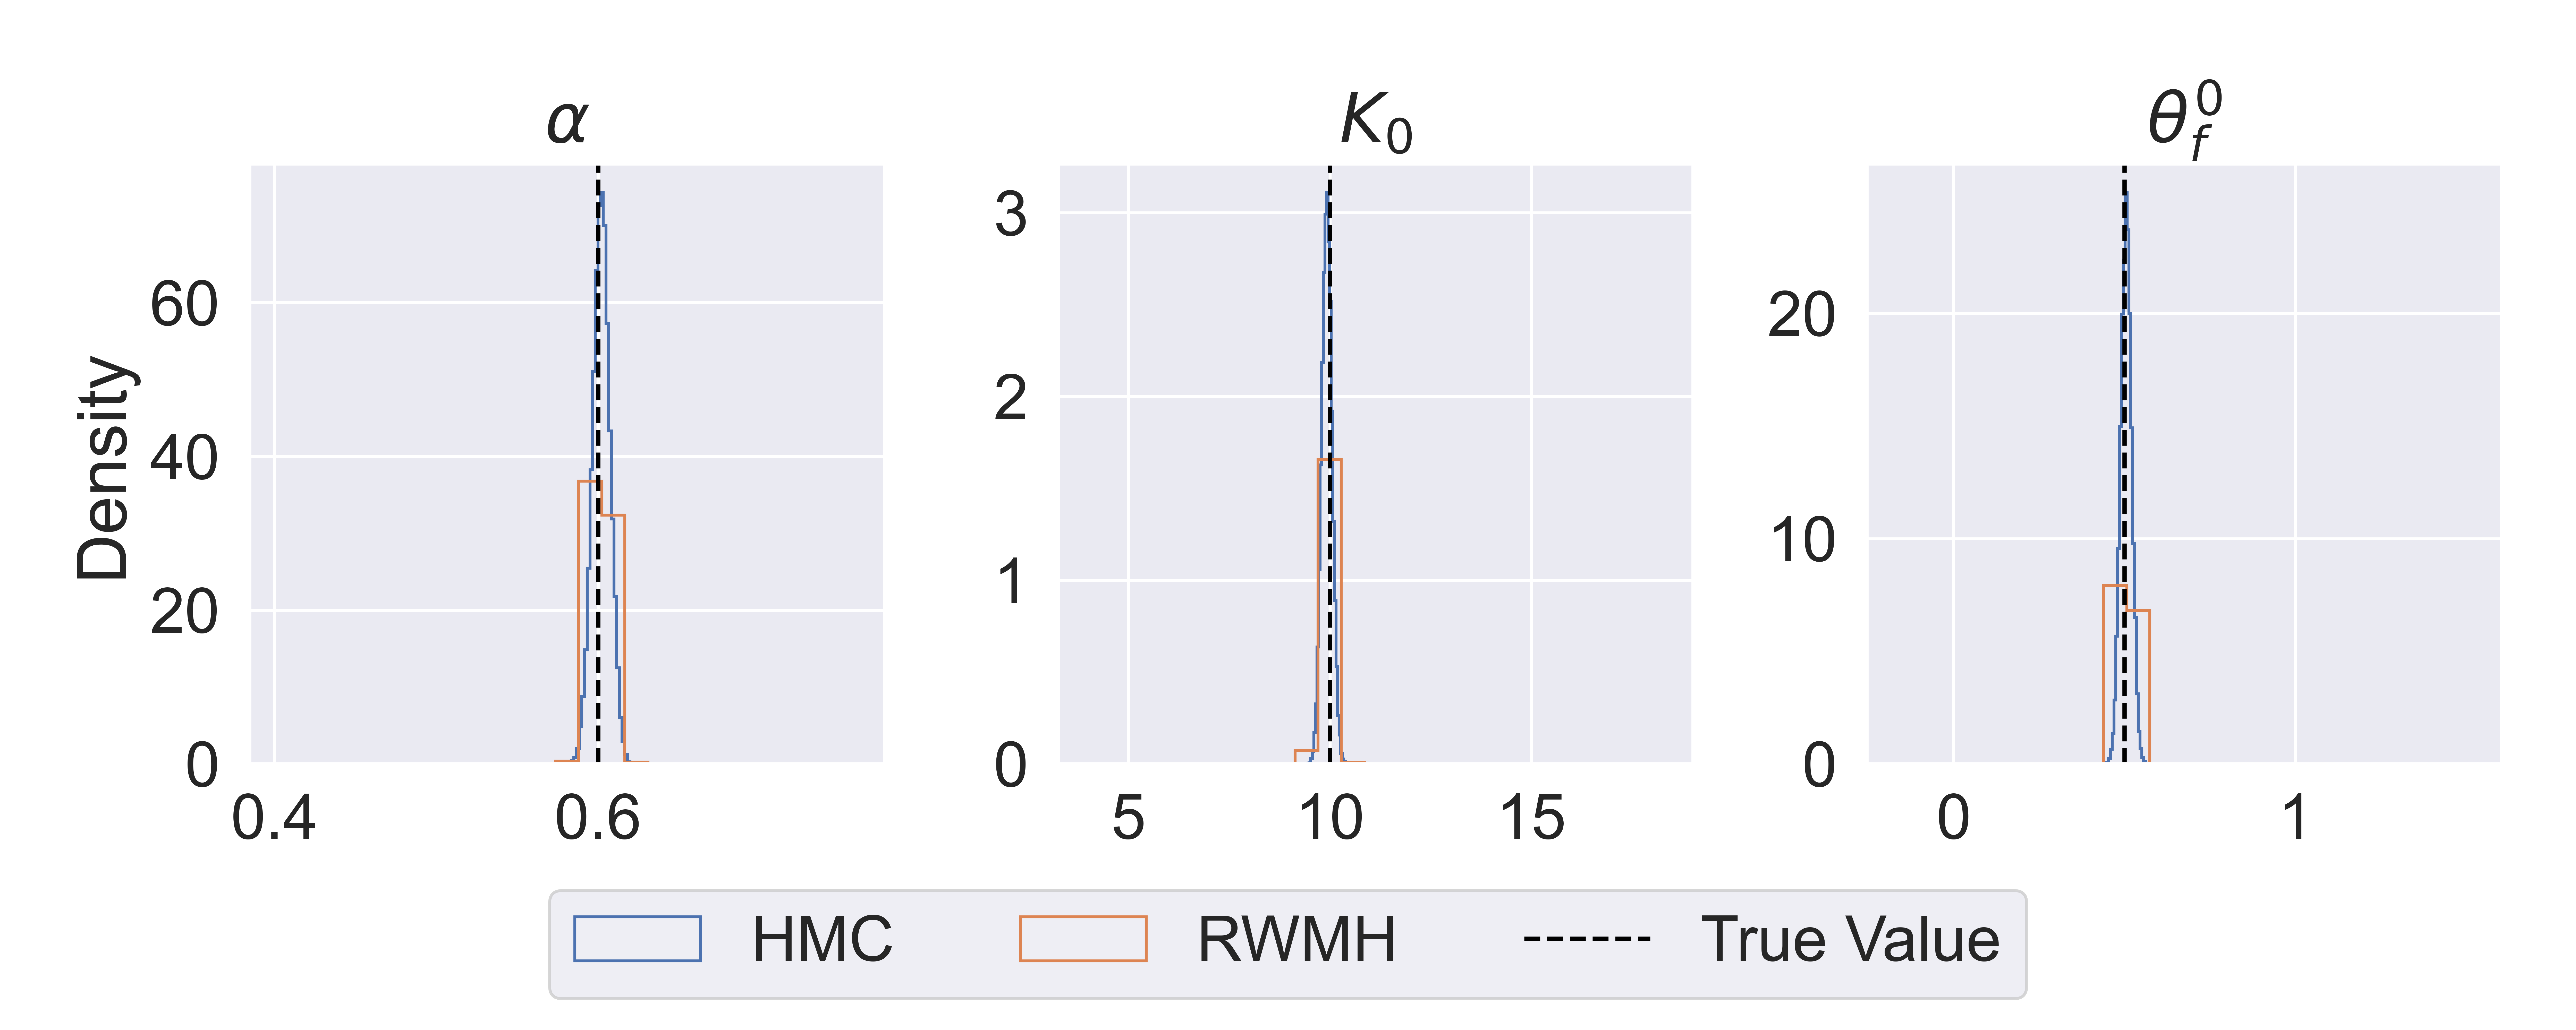
\includegraphics[width=0.95\textwidth]{figures/6-hmc-hist.png}
  \end{center}
  \caption[Marginal posteriors from NUTS and RWMH for the
  electron-transfer reaction]{Marginal posterior distributions for the
    three Butler--Volmer parameters obtained by NUTS (blue) and RWMH
    (orange) under equal computational budgets. Dashed lines indicate
    the true parameter values. Both samplers recover the correct
  posterior.}
  \label{fig:electron-posteriors}
\end{figure}

\begin{figure}[ht]
  \begin{center}
    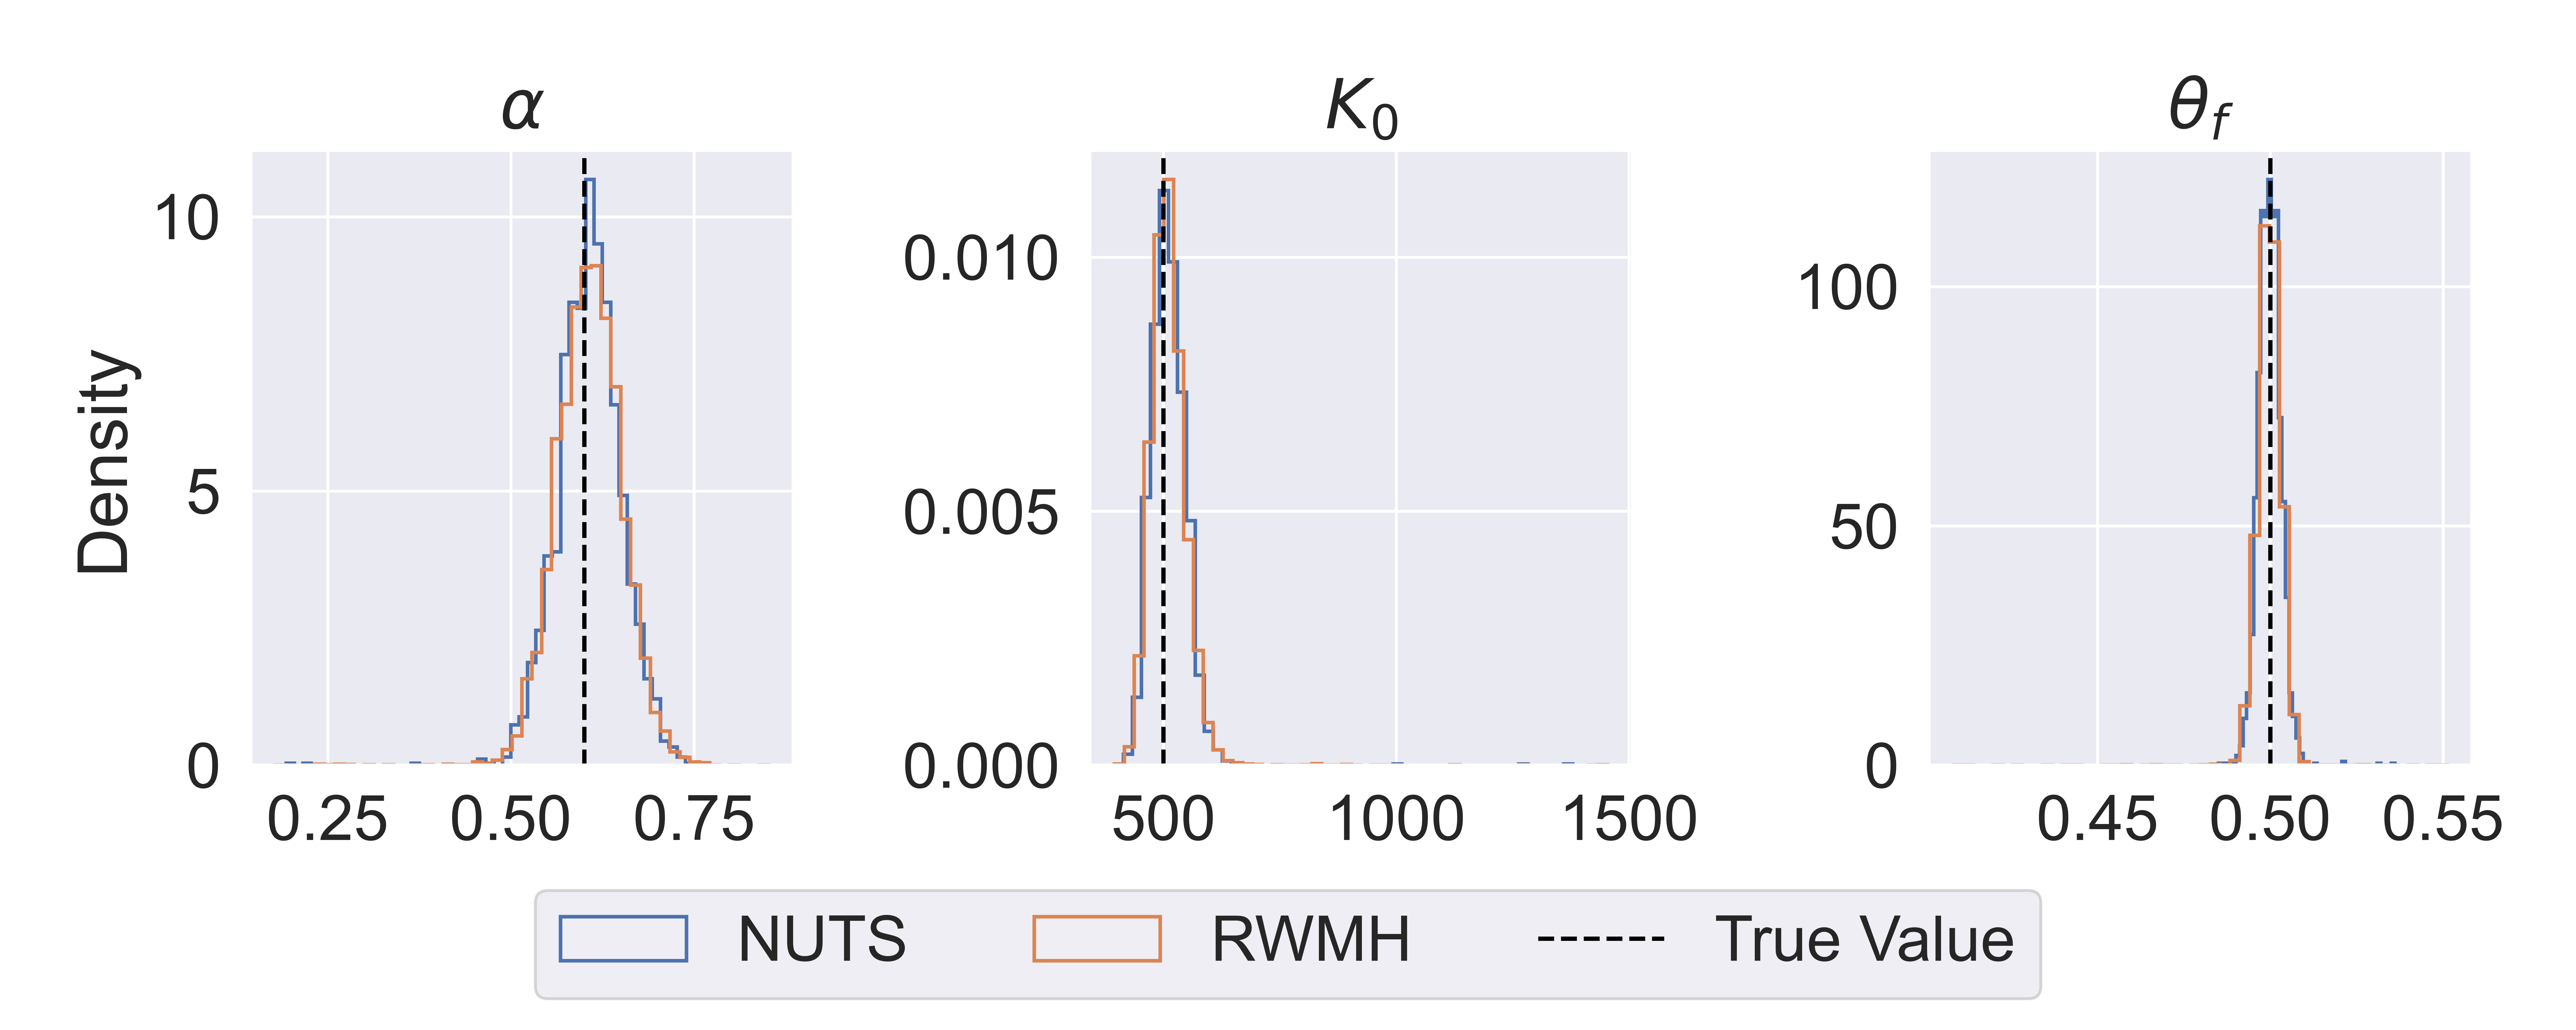
\includegraphics[width=0.95\textwidth]{figures/6-hmc-hist-rev.png}
  \end{center}
  \caption[Marginal posteriors from NUTS and RWMH for the
  electron-transfer reaction in the reversible regime]{Marginal
    posterior distributions for the
    three Butler--Volmer parameters obtained by NUTS (blue) and RWMH
    (orange) under equal computational budgets in the reversible
  regime. Dashed lines indicate the true parameter values.}
  \label{fig:electron-posteriors-rev}
\end{figure}

\Cref{fig:electron-current-fit} shows the simulated voltammogram
evaluated at the posterior mean from the NUTS chain against the true
parameter current. The close agreement confirms that the inferred
parameters reproduce the observed current response.

\begin{figure}[ht]
  \begin{center}
    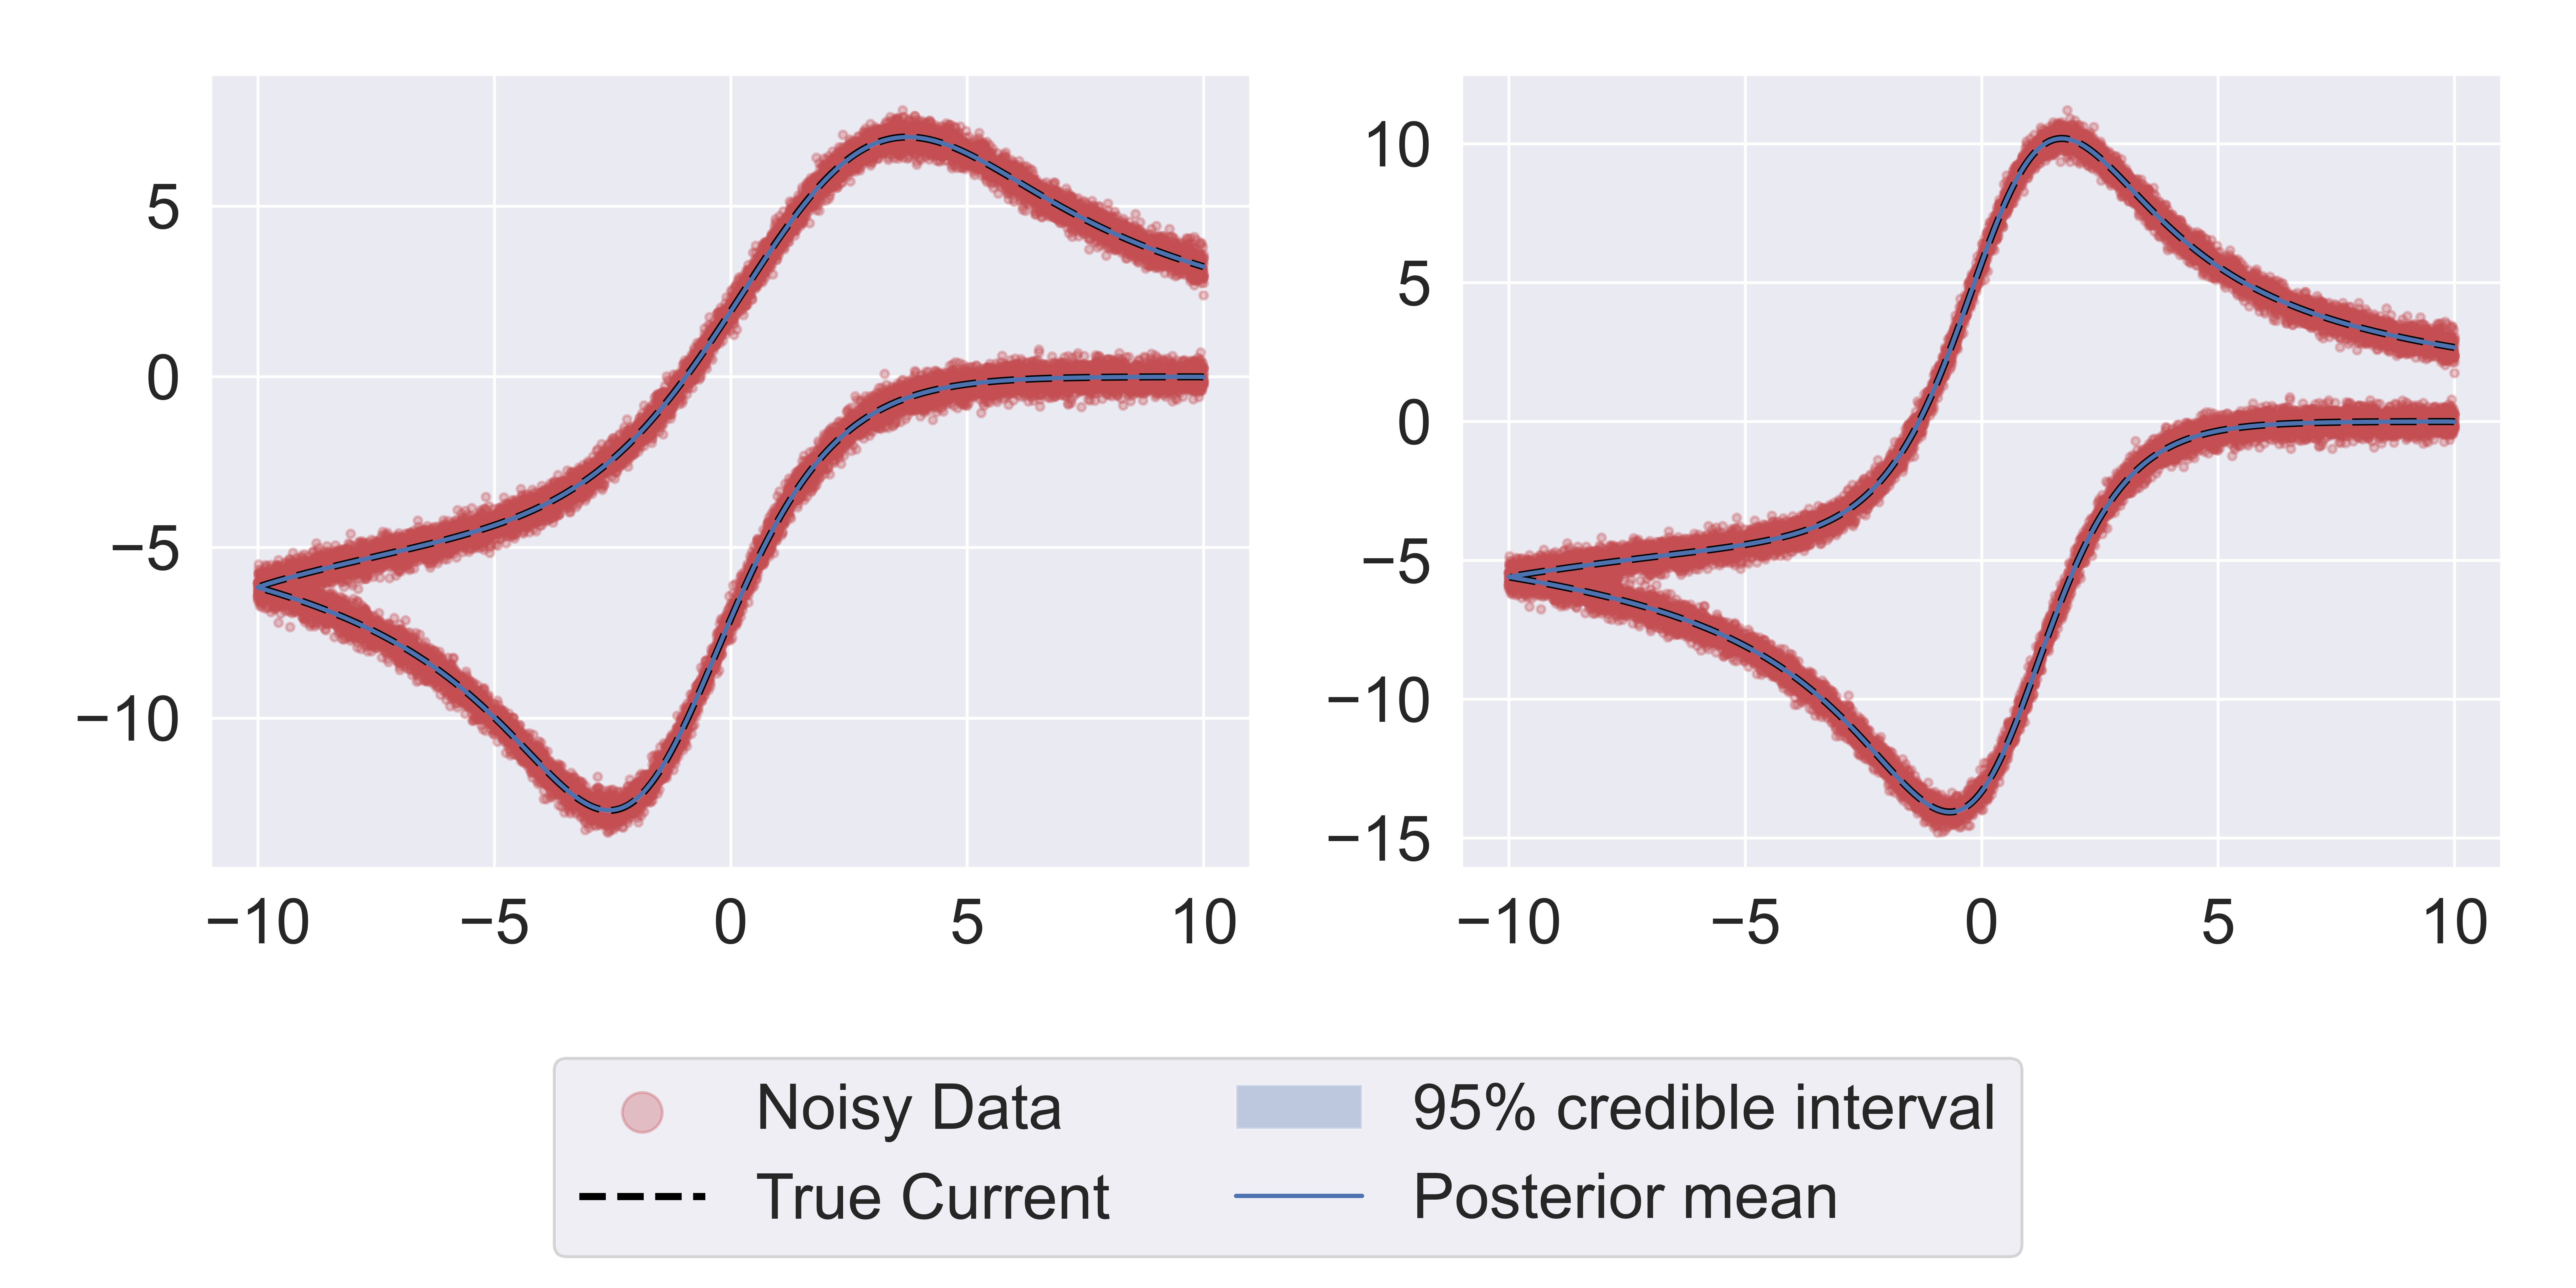
\includegraphics[width=0.7\textwidth]{figures/6-current-fit.png}
  \end{center}
  \caption[Posterior-mean current fit for the electron-transfer
  reaction]{Simulated voltammogram evaluated at the NUTS posterior
    mean, against the underlying true parameter voltammagrams. Left:
    Quasi-reversible reigime. Right: Reversible Reigime. The
    close agreement confirms that the inferred parameters reproduce the
  observed current.}
  \label{fig:electron-current-fit}
\end{figure}

\subsection{Effective Sample Size}

Any MCMC sampler produces serially correlated samples, so successive
draws carry less information than independent ones. The \emph{effective
sample size} (ESS)~\cite{gelman2013bayesian,geyer2011introduction}
quantifies the number of independent draws equivalent to the correlated
chain:
\begin{equation}
  \mathrm{ESS} = \frac{T}{1 + 2\sum_{k=1}^{\infty} \rho_k},
  \label{eq:ess}
\end{equation}
where $T$ is the total number of samples and $\rho_k$ is the
autocorrelation at lag~$k$.

\Cref{fig:electron-ess} compares the growth of ESS over the sampling
duration for NUTS and RWMH. The comparison is made on a normalised time
axis so that the two algorithms are compared at equal computational cost.
NUTS accumulates effective samples at a higher rate across all three
parameters. The advantage is most pronounced for~$K_0$, where NUTS
achieves roughly three times the ESS of RWMH at the end of the sampling
budget. \Cref{tab:electron-ess} reports the final ESS values for each
parameter.

\begin{table}[ht]
  \centering
  \begin{tabular}{lccc}
    \hline
    & $\alpha$ & $K_0$ & $\theta_f$ \\
    \hline
    NUTS & 2132.7 & 2986.7 & 2335.5 \\
    RWMH & 657.0 & 1634.0 & 761.0 \\
    \hline
  \end{tabular}
  \caption[Final ESS values for the electron-transfer reaction]{Effective
  sample size for each parameter at equal computational budget.}
  \label{tab:electron-ess}
\end{table}

\begin{figure}[ht]
  \begin{center}
    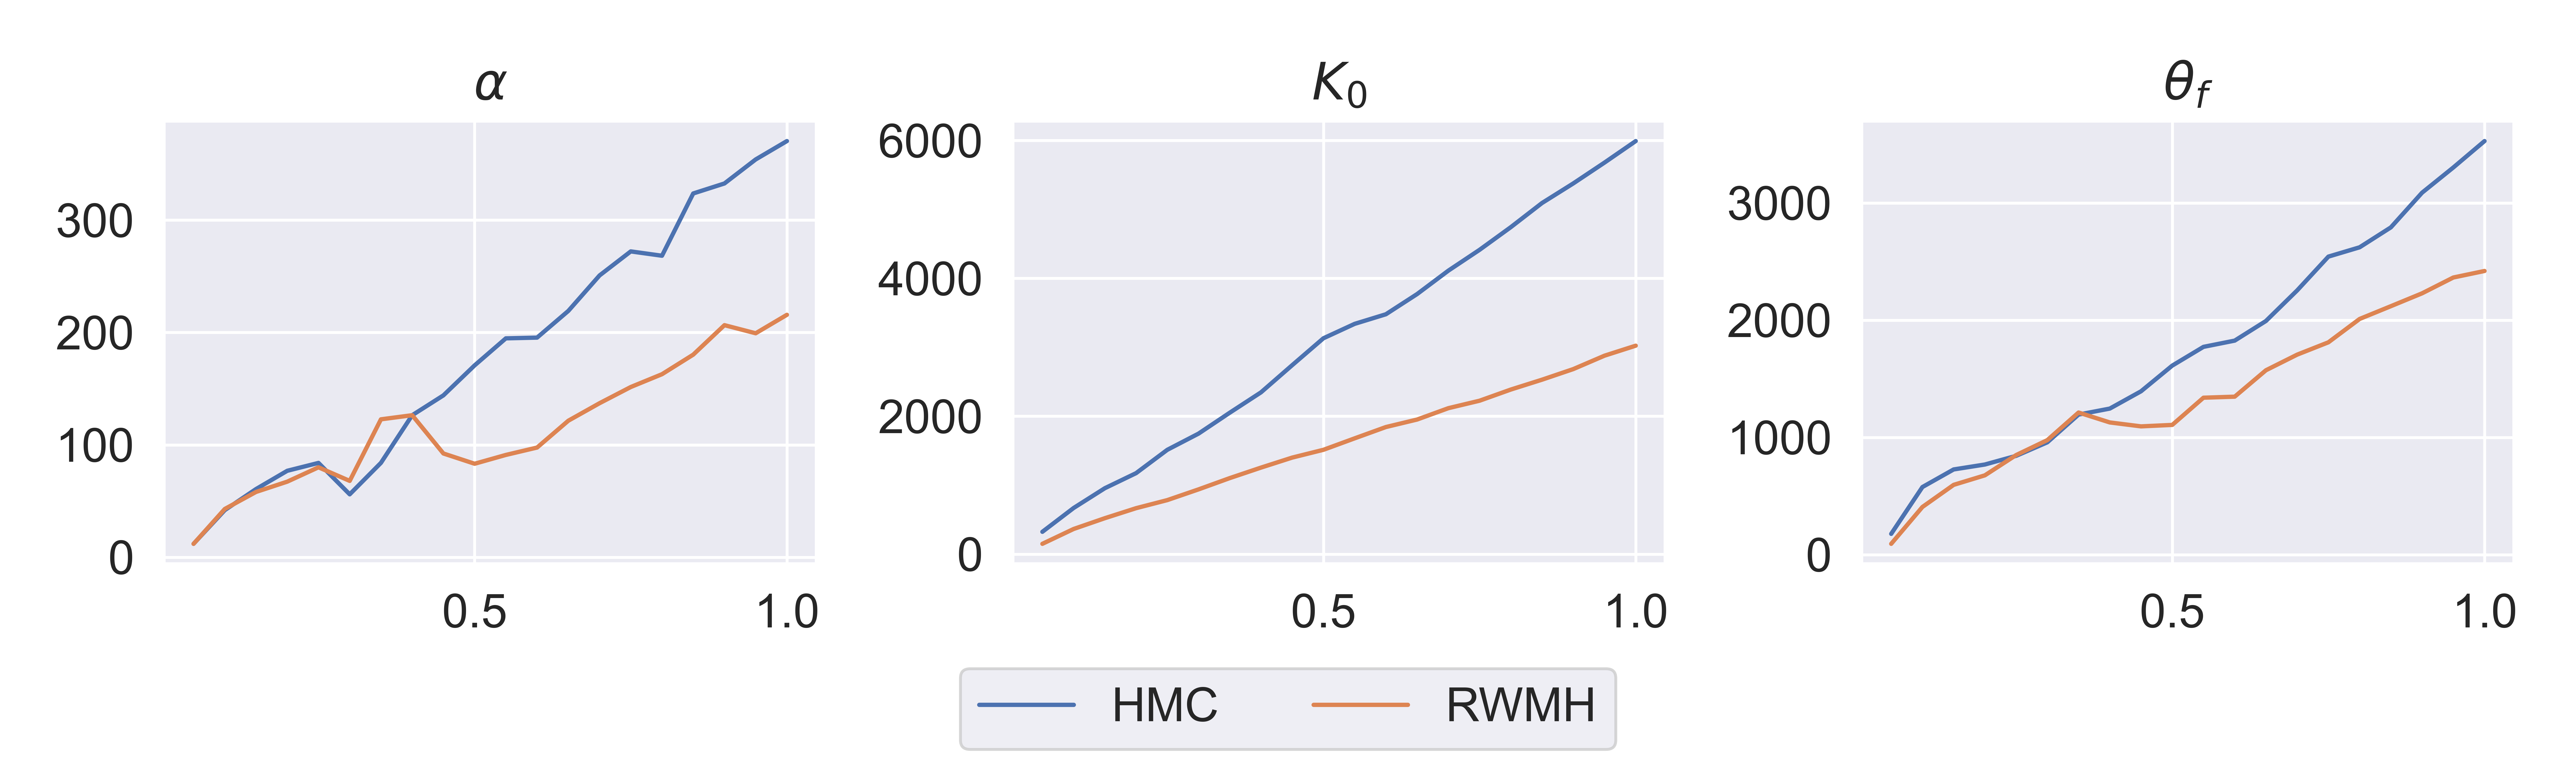
\includegraphics[width=0.95\textwidth]{figures/6-ess.png}
  \end{center}
  \caption[ESS comparison for NUTS and RWMH]{Effective sample size as a
    function of normalised computational time for NUTS (blue) and RWMH
    (orange), for each of the three Butler--Volmer parameters. The
    horizontal axis is normalised so that the two algorithms are compared
    at equal computational cost. NUTS achieves a higher ESS across all
  parameters, with the largest gain for~$K_0$.}
  \label{fig:electron-ess}
\end{figure}

With the inference framework now validated on the three-parameter
electron-transfer reaction, we apply it to reactions of increasing
complexity in the following chapters.

\chapter{Heterogeneous Reaction}

We will now be extending the methodology we have built up over the
previous chapters to a more complicated electrochemical reaciton
invoving two redox reaction and a heterogeneous chemical reaction
that couples the product and the reactant from the two equations
which occurs at the surface of the working electrode.

\begin{equation}\label{eq:hetero}
  \begin{gathered}
    \mathrm{A}+\mathrm{e}^{-} \rightleftarrows \mathrm{B} \\
    \mathrm{~B} \xrightarrow{k_{\text {het }}} \mathrm{C} \\
    \mathrm{C}+\mathrm{e}^{-} \rightleftarrows \mathrm{D}
  \end{gathered}
\end{equation}

This type of reaction appears in electroreduction of
halonitroaromatic compounds in aprotic media \cite{compton2014understanding}.

%TODO: Mention something about a more detailed description of these
% systems needs the consideration of adsorption / desorption which we
% deal with in the next chapter

%TODO: Mention that we now have the charge coefficient, rate constant
% formal potential for both reactions and heterogeneous rate constant
% as parameters

\begin{figure}
  \centering
  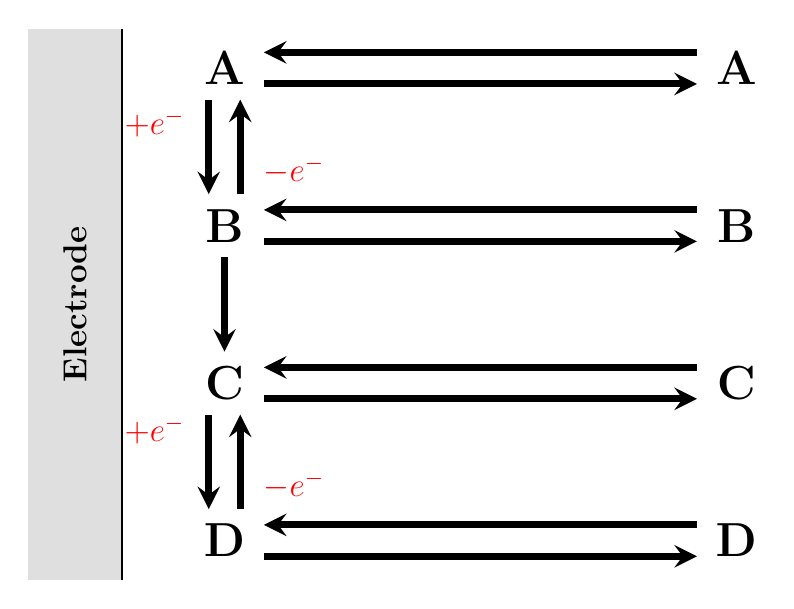
\begin{tikzpicture}[>=stealth, thick]
  % Electrode block
  \fill[gray!25] (-1.2, -1) rectangle (0, 6);
  \draw[thick] (0, -1) -- (0, 6);
  \node[rotate=90, font=\large\bfseries] at (-0.6, 2.5) {Electrode};
  % Species A row (top)
  \node[font=\LARGE\bfseries] at (1.3, 5.5) {A};
  \node[font=\LARGE\bfseries] at (7.8, 5.5) {A};
  % A: arrow from bulk towards electrode
  \draw[->, line width=2.5pt] (7.3, 5.7) -- (1.8, 5.7);
  % A: arrow from electrode towards bulk
  \draw[->, line width=2.5pt] (1.8, 5.3) -- (7.3, 5.3);
  % Species B row (bottom)
  \node[font=\LARGE\bfseries] at (1.3, 3.5) {B};
  \node[font=\LARGE\bfseries] at (7.8, 3.5) {B};
  % B: arrow from bulk towards electrode
  \draw[->, line width=2.5pt] (7.3, 3.7) -- (1.8, 3.7);
  % B: arrow from electrode towards bulk
  \draw[->, line width=2.5pt] (1.8, 3.3) -- (7.3, 3.3);
  % Electron transfer arrows AB
  \draw[->, line width=2.5pt] (1.1, 5.1) -- (1.1, 3.9);
  \node[right, font=\large] at (-0.1, 4.8) {\textcolor{red}{$+e^-$}};
  \draw[->, line width=2.5pt] (1.5, 3.9) -- (1.5, 5.1);
  \node[left, font=\large] at (2.7, 4.2) {\textcolor{red}{$-e^-$}};
  % Chemical Reaction B -> C
  \draw[->, line width=2.5pt] (1.3, 3.1) -- (1.3, 1.9);
  \node[font=\LARGE\bfseries] at (1.3, 1.5) {C};
  \node[font=\LARGE\bfseries] at (7.8, 1.5) {C};
  % C: arrow from bulk towards electrode
  \draw[->, line width=2.5pt] (7.3, 1.7) -- (1.8, 1.7);
  % C: arrow from electrode towards bulk
  \draw[->, line width=2.5pt] (1.8, 1.3) -- (7.3, 1.3);
  \node[font=\LARGE\bfseries] at (1.3, -0.5) {D};
  \node[font=\LARGE\bfseries] at (7.8, -0.5) {D};
  % D: arrow from bulk towards electrode
  \draw[->, line width=2.5pt] (7.3, -0.3) -- (1.8, -0.3);
  % D: arrow from electrode towards bulk
  \draw[->, line width=2.5pt] (1.8, -0.7) -- (7.3, -0.7);
  % Electron transfer arrows CD
  \draw[->, line width=2.5pt] (1.1, 1.1) -- (1.1, -0.1);
  \node[right, font=\large] at (-0.1, 0.9) {\textcolor{red}{$+e^-$}};
  \draw[->, line width=2.5pt] (1.5, -0.1) -- (1.5, 1.1);
  \node[left, font=\large] at (2.7, 0.2) {\textcolor{red}{$-e^-$}};
\end{tikzpicture}

  \caption{}
\end{figure}

\section{Mathematical Description}
We are able to express the reaction using the same non-dimensional
scheme as for the electron reaction. Only that we now need to model
the A, B, C and D species in separate governing equations. The
electrode boundary conditions change to:
\begin{equation}
  \begin{aligned}
    D_{\mathrm{A}}\left(\frac{\partial c_{\mathrm{A}}}{\partial
    x}\right)_{x=0} & =k_{\text {red }}^{(1)} c_{\mathrm{A}}(0,
    t)-k_{\mathrm{ox}}^{(1)} c_{\mathrm{B}}(0, t) \\
    D_{\mathrm{B}}\left(\frac{\partial c_{\mathrm{B}}}{\partial
    x}\right)_{x=0} & =-k_{\text {red }}^{(1)} c_{\mathrm{A}}(0,
    t)+k_{\mathrm{ox}}^{(1)} c_{\mathrm{B}}(0, t)+k_{\text {het }}
    c_{\mathrm{B}}(0, t) \\
    D_{\mathrm{C}}\left(\frac{\partial c_{\mathrm{C}}}{\partial
    x}\right)_{x=0} & =k_{\text {red }}^{(2)} c_{\mathrm{C}}(0,
    t)-k_{\mathrm{ox}}^{(2)} c_{\mathrm{D}}(0, t)-k_{\text {het }}
    c_{\mathrm{B}}(0, t) \\
    D_{\mathrm{D}}\left(\frac{\partial c_{\mathrm{D}}}{\partial
    x}\right)_{x=0} & =-k_{\text {red }}^{(2)} c_{\mathrm{C}}(0,
    t)+k_{\mathrm{ox}}^{(2)} c_{\mathrm{D}}(0, t)
  \end{aligned}
\end{equation}

Using the non-dimensional as we have described before and assuming
equal diffusion coefficients:
\begin{equation}
  \begin{aligned}
    & T>0, X=0: \\
    & \quad\left(\frac{\partial C_{\mathrm{A}}}{\partial
    X}\right)_{X=0}=K_{\text {red }}^{(1)} C_{\mathrm{A}}(0,
    T)-K_{\text {ox }}^{(1)} C_{\mathrm{B}}(0, T) \\
    & \quad\left(\frac{\partial C_{\mathrm{B}}}{\partial
    X}\right)_{X=0}=-K_{\text {red
    }}^{(1)} C_{\mathrm{A}}(0, T)+\left(K_{\text {ox }}^{(1)}+K_{\text
    {het }}\right) C_{\mathrm{B}}(0, T)\\
    & \quad\left(\frac{\partial C_{\mathrm{C}}}{\partial
    X}\right)_{X=0}=K_{\text {red
    }}^{(2)} C_{\mathrm{C}}(0, T)-K_{\text {ox }}^{(2)}
    C_{\mathrm{D}}(0, T)-K_{\text {het }} C_{\mathrm{B}}(0, T) \\
    & \quad\left(\frac{\partial C_{\mathrm{D}}}{\partial
    X}\right)_{X=0}=-K_{\text {red
    }}^{(2)} C_{\mathrm{C}}(0, T)+K_{\text {ox }}^{(2)}
    C_{\mathrm{D}}(0, T)
  \end{aligned}
\end{equation}
where the dimensionless rate constant of the heterogeneous chemical
reaction is given by
\begin{equation}
  K_{\mathrm{het}}=\frac{k_{\mathrm{het}} \epsilon}{D_{\mathrm{A}}}
\end{equation}

Notice the $K_{\mathrm{het}}$ term in the boundary for both
$\mathrm{B}$ and $\mathrm{C}$.
Regarding the current response the
total current will be given by the sum of the contribution of the
different heterogeneous \emph{electrochemical} reactions:
\begin{equation}
  \frac{I}{\mathrm{~F} A}
  =-\left\{D_{\mathrm{A}}\left(\frac{\partial
      c_{\mathrm{A}}}{\partial
    x}\right)_{x=0}+D_{\mathrm{C}}\left(\frac{\partial
    c_{\mathrm{C}}}{\partial x}\right)_{x=0}+k_{\text {het }}
  c_{\mathrm{B}}(0, t)\right\} \\
\end{equation}

% TODO: Mention the dimensionless conditions as everything is zero except A.

\chapter{Adsorption Reaction}\label{ch:adsorption}

This chapter applies the inference framework to a reaction involving
adsorption of the electroactive species onto the electrode surface.
Where \cref{ch:heterogeneous} treated an irreversible surface step
without explicit surface concentrations, the adsorption model
introduces surface coverage variables governed by ordinary differential
equations coupled to the diffusion PDE through the boundary conditions.
The Langmuir adsorption terms contain products of surface coverages and
surface concentrations, making the discrete system nonlinear and
preventing a direct banded solve. We compare three discretisation
strategies -- Newton--Raphson, explicit linearisation, and backward
implicit linearisation. Such systems arise experimentally when an
electrode is modified with a redox-active film (for example, a
  self-assembled monolayer of ferrocene-terminated thiols on
gold~\cite{compton2014understanding}) and the
voltammetry is performed in a blank electrolyte. The parameter space
grows to nine dimensions, completing the sequence $3 \to 7 \to 9$ that
structures the NUTS--RWMH comparison.

\section{Reaction Scheme}\label{sec:ads-scheme}

We consider a single electron transfer in which both the reactant
$\mathrm{A}$ and the product $\mathrm{B}$ can adsorb on the electrode
surface \cite{compton2014understanding}:
\begin{equation}\label{eq:ads-scheme}
  \mathrm{A} + \mathrm{e}^{-} \rightleftharpoons \mathrm{B}.
\end{equation}
The electron transfer can proceed through both the solution-phase
species (with rate constants $k_{\mathrm{red/ox}}^{\mathrm{sol}}$) and
the surface-bound species (with rate constants
$k_{\mathrm{red/ox}}^{\mathrm{ads}}$). Each species adsorbs onto and
desorbs from the electrode surface with rate constants
$k_{\mathrm{ads}}^{j}$ and $k_{\mathrm{des}}^{j}$, competing for a
finite number of surface sites characterised by the maximum surface
concentration $\Gamma_{\mathrm{max}}$ (\cref{fig:ads-schematic}).

\begin{figure}
  \centering
  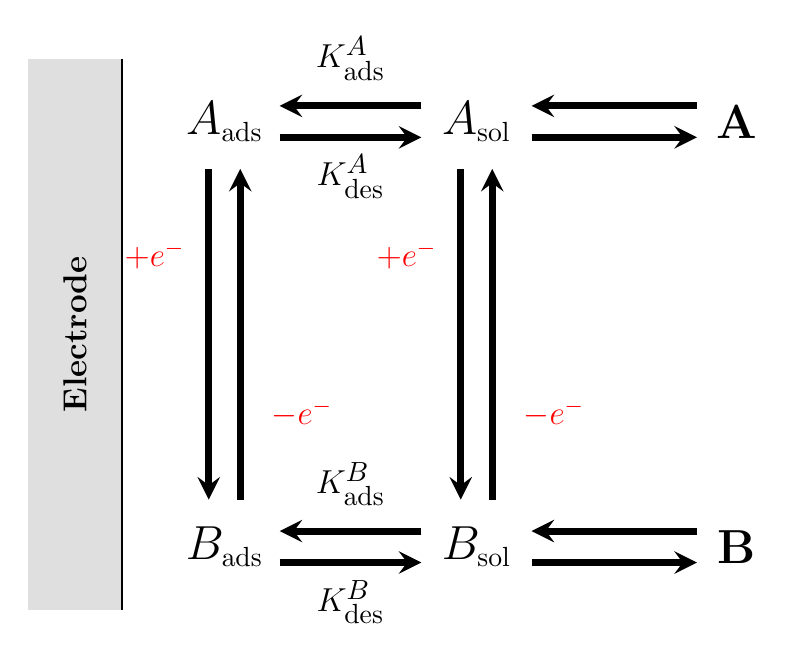
\begin{tikzpicture}[>=stealth, thick]
  % Electrode block
  \fill[gray!25] (-1.2, -1) rectangle (0, 6);
  \draw[thick] (0, -1) -- (0, 6);
  \node[rotate=90, font=\large\bfseries] at (-0.6, 2.5) {Electrode};

  % Species A row (top)
  \node[font=\LARGE\bfseries] at (1.3, 5.2) {$A_{\scriptscriptstyle
  \mathrm{ads}}$};
  \node[font=\LARGE\bfseries] at (4.5, 5.2) {$A_{\scriptscriptstyle
  \mathrm{sol}}$};
  \node[font=\LARGE\bfseries] at (7.8, 5.2) {A};

  % A: arrows
  \draw[->, line width=2.5pt] (7.3, 5.4) -- (5.2, 5.4);
  \draw[->, line width=2.5pt] (3.8, 5.4) -- (2.0, 5.4);
  \node[font=\LARGE\bfseries] at (2.9, 6.0) {$\scriptstyle K_{\scriptscriptstyle
  \mathrm{ads}}^{A}$};

  \draw[->, line width=2.5pt] (2.0, 5.0) -- (3.8, 5.0);
  \draw[->, line width=2.5pt] (5.2, 5.0) -- (7.3, 5.0);
  \node[font=\LARGE\bfseries] at (2.9, 4.5) {$\scriptstyle K_{\scriptscriptstyle
  \mathrm{des}}^{A}$};

  % Species B row (bottom)
  \node[font=\LARGE\bfseries] at (1.3, -0.2) {$B_{\scriptscriptstyle
  \mathrm{ads}}$};
  \node[font=\LARGE\bfseries] at (4.5, -0.2) {$B_{\scriptscriptstyle
  \mathrm{sol}}$};
  \node[font=\LARGE\bfseries] at (7.8, -0.2) {B};

  % B: arrows
  \draw[->, line width=2.5pt] (7.3, 0.0) -- (5.2, 0.0);
  \draw[->, line width=2.5pt] (3.8, 0.0) -- (2.0, 0.0);
  \node[font=\LARGE\bfseries] at (2.9, 0.6) {$\scriptstyle K_{\scriptscriptstyle
  \mathrm{ads}}^{B}$};

  \draw[->, line width=2.5pt] (2.0, -0.4) -- (3.8, -0.4);
  \draw[->, line width=2.5pt] (5.2, -0.4) -- (7.3, -0.4);

  \node[font=\LARGE\bfseries] at (2.9, -0.9) {$\scriptstyle
    K_{\scriptscriptstyle
  \mathrm{des}}^{B}$};

  % Electron solution transfer arrows
  \draw[->, line width=2.5pt] (4.3, 4.6) -- (4.3, 0.4);
  \node[left, font=\large] at (6.0, 1.5) {\textcolor{red}{$-e^-$}};
  \draw[->, line width=2.5pt] (4.7, 0.4) -- (4.7, 4.6);
  \node[right, font=\large] at (3.1, 3.5) {\textcolor{red}{$+e^-$}};

  % Electron adsorption transfer arrows
  \draw[->, line width=2.5pt] (1.1, 4.6) -- (1.1, 0.4);
  \node[left, font=\large] at (2.8, 1.5) {\textcolor{red}{$-e^-$}};
  \draw[->, line width=2.5pt] (1.5, 0.4) -- (1.5, 4.6);
  \node[right, font=\large] at (-0.1, 3.5) {\textcolor{red}{$+e^-$}};

\end{tikzpicture}

  \caption[Schematic of the adsorption reaction]{Schematic of the
    adsorption reaction mechanism. Species $\mathrm{A}$ and $\mathrm{B}$
    exist in both a solution phase and a surface-bound (adsorbed) phase.
    Electron transfer can occur between both solution-phase and
    adsorbed species. Adsorption and desorption exchange species between
  the two phases.}
  \label{fig:ads-schematic}
\end{figure}

The solution-phase and adsorbed electron transfers are each
characterised by their own transfer coefficient and rate constant:
$(\alpha^{\mathrm{sol}},\, K_0^{\mathrm{sol}})$ and
$(\alpha^{\mathrm{ads}},\, K_0^{\mathrm{ads}})$ respectively. The nine
parameters to be inferred are
\begin{equation}\label{eq:ads-params}
  \phi = \bigl(\alpha^{\mathrm{sol}},\, K_0^{\mathrm{sol}},\,
    \theta_f^{\mathrm{sol}},\,
    \alpha^{\mathrm{ads}},\, K_0^{\mathrm{ads}},\,
    K_{\mathrm{ads}}^{\mathrm{A}},\, K_{\mathrm{des}}^{\mathrm{A}},\,
    K_{\mathrm{ads}}^{\mathrm{B}},\, K_{\mathrm{des}}^{\mathrm{B}}
  \bigr) \in \mathbb{R}^9.
\end{equation}
The saturation parameter $\beta = c_\mathrm{A}^*\,r_e/
\Gamma_{\mathrm{max}}$ is treated as known and fixed at $\beta = 1$.

\section{Mathematical Description}\label{sec:ads-maths}

\subsection{Governing Equations}

The transport of $\mathrm{A}$ and $\mathrm{B}$ in solution is governed
by the same dimensionless diffusion equation as in
\cref{eq:nd_diffusion}:
\begin{equation}\label{eq:ads-diffusion}
  \frac{\partial C_j}{\partial T} = \frac{\partial^2 C_j}{\partial X^2},
  \qquad j \in \{\mathrm{A},\,\mathrm{B}\}.
\end{equation}
Unlike the heterogeneous reaction of \cref{ch:heterogeneous}, there are
no kinetic source terms in the bulk. All coupling between the species
enters through the boundary conditions at the electrode surface.

\subsection{Surface Coverage Equations}

The surface coverages $\xi_j = \Gamma_j / \Gamma_{\mathrm{max}}$
evolve according to
\begin{equation}\label{eq:ads-coverage-ode}
  \begin{aligned}
    \frac{\mathrm{d}\xi_\mathrm{A}}{\mathrm{d}T}
    &= -K_{\mathrm{red}}^{\mathrm{ads}}\,\xi_\mathrm{A}
    + K_{\mathrm{ox}}^{\mathrm{ads}}\,\xi_\mathrm{B}
    + K_{\mathrm{ads}}^{\mathrm{A}}\,C_{0,\mathrm{A}}
    \bigl[1 - (\xi_\mathrm{A} + \xi_\mathrm{B})\bigr]
    - K_{\mathrm{des}}^{\mathrm{A}}\,\xi_\mathrm{A}, \\[4pt]
    \frac{\mathrm{d}\xi_\mathrm{B}}{\mathrm{d}T}
    &= K_{\mathrm{red}}^{\mathrm{ads}}\,\xi_\mathrm{A}
    - K_{\mathrm{ox}}^{\mathrm{ads}}\,\xi_\mathrm{B}
    + K_{\mathrm{ads}}^{\mathrm{B}}\,C_{0,\mathrm{B}}
    \bigl[1 - (\xi_\mathrm{A} + \xi_\mathrm{B})\bigr]
    - K_{\mathrm{des}}^{\mathrm{B}}\,\xi_\mathrm{B},
  \end{aligned}
\end{equation}
where $C_{0,j} = C_j(T, 0)$ is the surface concentration in solution.
The first two terms in each equation are the adsorbed electron transfer;
the third is Langmuir adsorption, with $[1 - (\xi_\mathrm{A} +
\xi_\mathrm{B})]$ the fraction of unoccupied sites; the fourth is
desorption.

\subsection{Electrode Boundary Conditions}

The surface flux of each species is determined by the solution-phase
electron transfer and the net adsorption/desorption flux:
\begin{equation}\label{eq:ads-bc}
  \begin{aligned}
    \left(\frac{\partial C_\mathrm{A}}{\partial X}\right)_{X=0}
    &= K_{\mathrm{red}}^{\mathrm{sol}}\,C_{0,\mathrm{A}}
    - K_{\mathrm{ox}}^{\mathrm{sol}}\,C_{0,\mathrm{B}}
    + K_{\mathrm{ads}}^{\mathrm{A}}\,C_{0,\mathrm{A}}
    \bigl[1 - (\xi_\mathrm{A} + \xi_\mathrm{B})\bigr]
    - K_{\mathrm{des}}^{\mathrm{A}}\,\xi_\mathrm{A}, \\[4pt]
    \left(\frac{\partial C_\mathrm{B}}{\partial X}\right)_{X=0}
    &= \frac{1}{d_\mathrm{B}}\Bigl\{
      -K_{\mathrm{red}}^{\mathrm{sol}}\,C_{0,\mathrm{A}}
      + K_{\mathrm{ox}}^{\mathrm{sol}}\,C_{0,\mathrm{B}}
      + K_{\mathrm{ads}}^{\mathrm{B}}\,C_{0,\mathrm{B}}
      \bigl[1 - (\xi_\mathrm{A} + \xi_\mathrm{B})\bigr]
      - K_{\mathrm{des}}^{\mathrm{B}}\,\xi_\mathrm{B}
    \Bigr\}.
  \end{aligned}
\end{equation}
The dimensionless rate constants follow the Butler--Volmer form:
\begin{equation}\label{eq:ads-kred-kox}
  \begin{aligned}
    K_{\mathrm{red}}^{\mathrm{sol}}
    &= K_0^{\mathrm{sol}}
    \exp\!\bigl[-\alpha^{\mathrm{sol}}\bigl(\theta(T) -
    \theta_f^{\mathrm{sol}}\bigr)\bigr],
    &\qquad
    K_{\mathrm{ox}}^{\mathrm{sol}}
    &= K_0^{\mathrm{sol}}
    \exp\!\bigl[(1-\alpha^{\mathrm{sol}})\bigl(\theta(T) -
    \theta_f^{\mathrm{sol}}\bigr)\bigr],
    \\[4pt]
    K_{\mathrm{red}}^{\mathrm{ads}}
    &= K_0^{\mathrm{ads}}
    \exp\!\bigl[-\alpha^{\mathrm{ads}}\bigl(\theta(T) -
    \theta_f^{\mathrm{ads}}\bigr)\bigr],
    &\qquad
    K_{\mathrm{ox}}^{\mathrm{ads}}
    &= K_0^{\mathrm{ads}}
    \exp\!\bigl[(1-\alpha^{\mathrm{ads}})\bigl(\theta(T) -
    \theta_f^{\mathrm{ads}}\bigr)\bigr],
  \end{aligned}
\end{equation}
where $K_0^{\mathrm{sol}} = k_0^{\mathrm{sol}}\,r_e/ D_\mathrm{A}$
and $K_0^{\mathrm{ads}} = k_0^{\mathrm{ads}}\,r_e^2 / D_\mathrm{A}$.
The formal potentials of the two couples are related by thermodynamic
consistency \cite{compton2014understanding}:
\begin{equation}\label{eq:ads-thetaf-relation}
  \theta_f^{\mathrm{ads}} = \theta_f^{\mathrm{sol}}
  - \ln\!\left(
    \frac{K_{\mathrm{ads}}^{\mathrm{A}} / K_{\mathrm{des}}^{\mathrm{A}}}
    {K_{\mathrm{ads}}^{\mathrm{B}} / K_{\mathrm{des}}^{\mathrm{B}}}
  \right).
\end{equation}
This is not an additional free parameter: $\theta_f^{\mathrm{ads}}$ is
determined by $\theta_f^{\mathrm{sol}}$ and the four
adsorption/desorption dimensionless rate constants already in~$\phi$
which are of the form
\begin{equation}\label{eq:ads-kads-kdes}
  K_{\mathrm{ads}}^{j}
  = \frac{k_{\mathrm{ads}}^{j}\,\Gamma_{\mathrm{max}}\,r_e}
  {D_\mathrm{A}},
  \qquad
  K_{\mathrm{des}}^{j}
  = \frac{k_{\mathrm{des}}^{j}\,\Gamma_{\mathrm{max}}\,r_e}
  {c_\mathrm{A}^*\,D_\mathrm{A}}.
\end{equation}

\subsection{Initial Conditions}

Initially only species $\mathrm{A}$ is present in solution at its bulk
concentration: $C_\mathrm{A}(0, X) = 1$, $C_\mathrm{B}(0, X) = 0$.
The initial surface coverages are set by the Langmuir equilibrium:
\begin{equation}\label{eq:ads-ic-coverage}
  \xi_\mathrm{A}(0) =
  \frac{K_{\mathrm{ads}}^{\mathrm{A}} / K_{\mathrm{des}}^{\mathrm{A}}}
  {1 + K_{\mathrm{ads}}^{\mathrm{A}} / K_{\mathrm{des}}^{\mathrm{A}}
    + C_\mathrm{B}^*\, K_{\mathrm{ads}}^{\mathrm{B}} /
  K_{\mathrm{des}}^{\mathrm{B}}},
  \qquad
  \xi_\mathrm{B}(0) =
  \frac{C_\mathrm{B}^*\, K_{\mathrm{ads}}^{\mathrm{B}} /
  K_{\mathrm{des}}^{\mathrm{B}}}
  {1 + K_{\mathrm{ads}}^{\mathrm{A}} / K_{\mathrm{des}}^{\mathrm{A}}
    + C_\mathrm{B}^*\, K_{\mathrm{ads}}^{\mathrm{B}} /
  K_{\mathrm{des}}^{\mathrm{B}}}.
\end{equation}

We set $C_\mathrm{B}^* = 0$ and thus $\xi_\mathrm{B}(0) = 0$.

\subsection{Current}

The measured current has contributions from both the solution-phase and
adsorbed electron transfers:
\begin{equation}\label{eq:ads-current}
  \frac{I}{\pi r_e F D_\mathrm{A} c_\mathrm{A}^*}
  = -\left\{
    \left(\frac{\partial C_\mathrm{A}}{\partial X}\right)_{X=0}
    - \frac{1}{\beta}
    \frac{\mathrm{d}\xi_\mathrm{A}}{\mathrm{d}T}
  \right\}.
\end{equation}
The first term is the diffusive flux; the second accounts for charge
transferred by the conversion of adsorbed $\mathrm{A}$ to adsorbed
$\mathrm{B}$.

\section{Nonlinearity and Discretisation}\label{sec:ads-disc}

The Langmuir terms in \cref{eq:ads-coverage-ode,eq:ads-bc} contain
products of the unknown surface concentrations $C_{0,j}$ and surface
coverages $\xi_j$ at the current timestep. After backward Euler
discretisation these become products of unknowns at timestep~$k$,
making the algebraic system nonlinear -- in contrast to
\cref{ch:heterogeneous}, where all coupling was linear and the system
could be solved directly.

\subsection{Newton--Raphson Solver}\label{sec:ads-newton}

We order the unknowns as $\mathbf{x} = (\xi_\mathrm{A}^k,\,
  \xi_\mathrm{B}^k,\, C_{0,\mathrm{A}}^k,\, C_{0,\mathrm{B}}^k,\,
\ldots,\, C_{n-1,\mathrm{A}}^k,\, C_{n-1,\mathrm{B}}^k)^T$ and solve
the nonlinear residual $\mathbf{F}(\mathbf{x}) = 0$ by Newton--Raphson
iteration, using the previous timestep's solution as the initial guess.
After a preliminary row elimination to decouple the surface coverage
from the far-field equations~\cite{compton2014understanding}, the
Jacobian reduces to pentadiagonal form. We solve to tight tolerances
($r_{\mathrm{tol}} = 10^{-10}$, $a_{\mathrm{tol}} = 10^{-12}$) so
that this solver serves as the ground-truth reference. One could fix
the iteration count to make the solver traceable by reverse-mode AD,
but this neither guarantees convergence nor avoids the cost of
differentiating through every Newton step. We therefore require a
linearised alternative for inference.

\subsection{Alternative Solvers}\label{sec:ads-alt-solvers}

Two strategies linearise the nonlinear terms at each timestep, producing
systems solvable directly and differentiable through.

\paragraph{Explicit linearisation.}
The products $C_{0,j}^k\,[1 - (\xi_\mathrm{A}^k +
\xi_\mathrm{B}^k)]$ are approximated by evaluating the surface
coverage at the previous timestep:
\begin{equation}\label{eq:ads-explicit}
  C_{0,j}^k\,\bigl[1 - (\xi_\mathrm{A}^k + \xi_\mathrm{B}^k)\bigr]
  \approx
  C_{0,j}^k\,\bigl[1 - (\xi_\mathrm{A}^{k-1} + \xi_\mathrm{B}^{k-1})\bigr].
\end{equation}
This is first-order in $\Delta T$ and accurate when the surface
coverage does not change rapidly between timesteps.

Following Britz~\cite{britz2016digital}, the product is expanded to
first order about the previous-timestep values:
\begin{equation}\label{eq:ads-britz}
  C_{0,j}^k\,\xi_l^k
  \approx
  C_{0,j}^k\,\xi_l^{k-1}
  + C_{0,j}^{k-1}\,\xi_l^k
  - C_{0,j}^{k-1}\,\xi_l^{k-1}.
\end{equation}
This retains linear coupling to both unknowns at timestep~$k$, also
first-order in $\Delta T$ but with more implicit coupling than the
explicit scheme. Both alternatives produce a pentadiagonal system after
row elimination which is compatible with the adjoint framework of
\cref{ch:adjoint}.

\subsection{Solver Comparison}\label{sec:ads-solver-comparison}

\Cref{fig:ads-solver-comparison} compares the two AD-compatible solvers
against the Newton reference. The backward implicit scheme achieves
errors of order $10^{-7}$ across most of the sweep, compared with
$10^{-3}$ for the explicit scheme. For both solvers, the error
increases when we have a fast change in the gradient of the current.

\begin{figure}[ht]
  \centering
  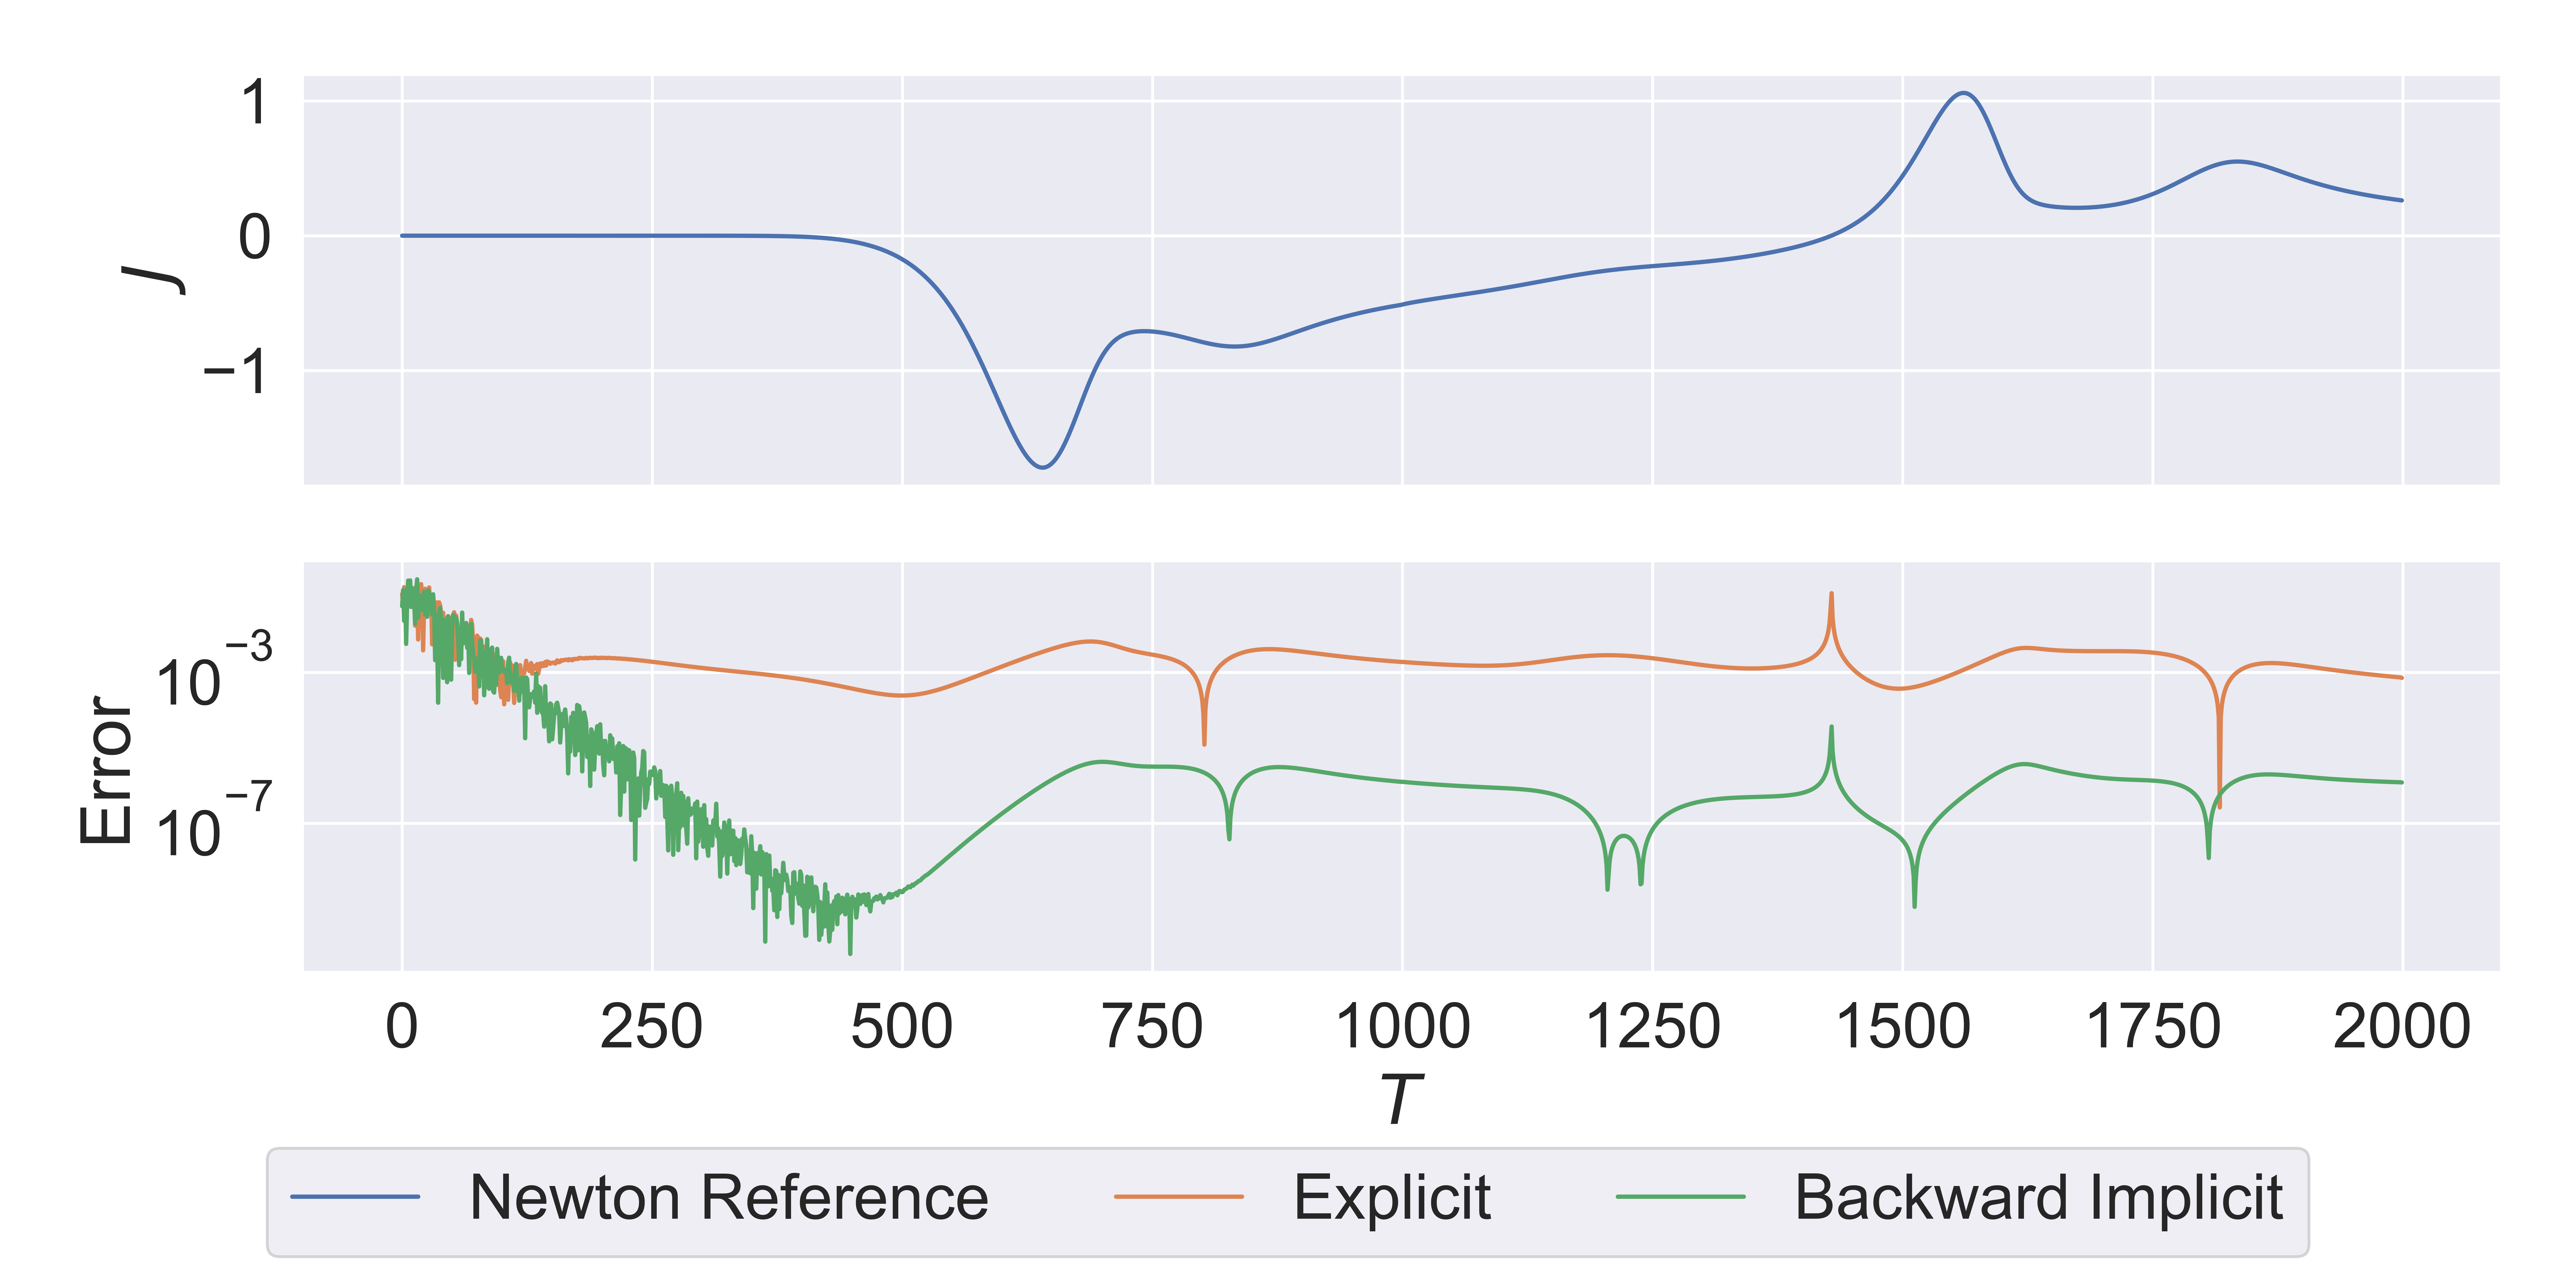
\includegraphics[width=0.95\textwidth]{figures/8-solver-comparison.png}
  \caption[Solver comparison for the adsorption reaction]{Top:
    Reference Newton current against time. Bottom: Absolute
    relative error of the explicit (orange) and backward implicit (green)
    solvers against the Newton reference at each timestep. The backward
    implicit scheme is three to four orders of magnitude more accurate
  across most of the sweep.}
  \label{fig:ads-solver-comparison}
\end{figure}

The backward implicit solver is slower than the explicit solver
(80\,ms vs 60\,ms per forward solve). This 33\% overhead is
acceptable given the accuracy gain, and we adopt the backward implicit
scheme for all inference runs.

\section{Inference Setup}\label{sec:ads-inference}

The inference workflow follows \cref{sec:workflow} without modification.
The transfer coefficients are logit-transformed, the rate constants
log-transformed, and $\theta_f^{\mathrm{sol}}$ left untransformed.
Synthetic data are generated using the Newton solver at the true
parameter values
\begin{equation}\label{eq:ads-true-params}
  \phi^* = (0.5,\; 10^{-3},\; 0.0,\; 0.45,\; 0.5,\;
  4.5,\; 1.0,\; 1.0,\; 1.0),
\end{equation}
with dimensionless scan rate $\sigma = 10$ and noise level
$\eta = 0.02$. The scan rate is two orders of magnitude lower than the
$\sigma = 1000$ used in the preceding chapters: adsorption and
desorption operate on a slower timescale than electron transfer, and at
high scan rates the potential sweeps too fast for adsorption to respond,
rendering the voltammogram insensitive to the adsorption rate constants.

\section{Results}\label{sec:ads-results}

\subsection{Solver Verification}\label{sec:ads-verification}

We verify the forward solver against the analytical solution for a pure
monolayer -- a system in which all electroactive material is
pre-adsorbed and no solution-phase electron transfer occurs. For a
fully reversible adsorbed redox couple the dimensionless current is
\cite{chen2026differentiable}
\begin{equation}\label{eq:ads-monolayer-analytical}
  J = \mp\,\frac{\exp(-\theta)}{(1 + \exp(-\theta))^2},
\end{equation}
where the upper sign refers to the cathodic scan and the lower to the
anodic scan. \Cref{fig:ads-verification} confirms that the numerical
solution reproduces the full analytical trajectory.

\begin{figure}[ht]
  \centering
  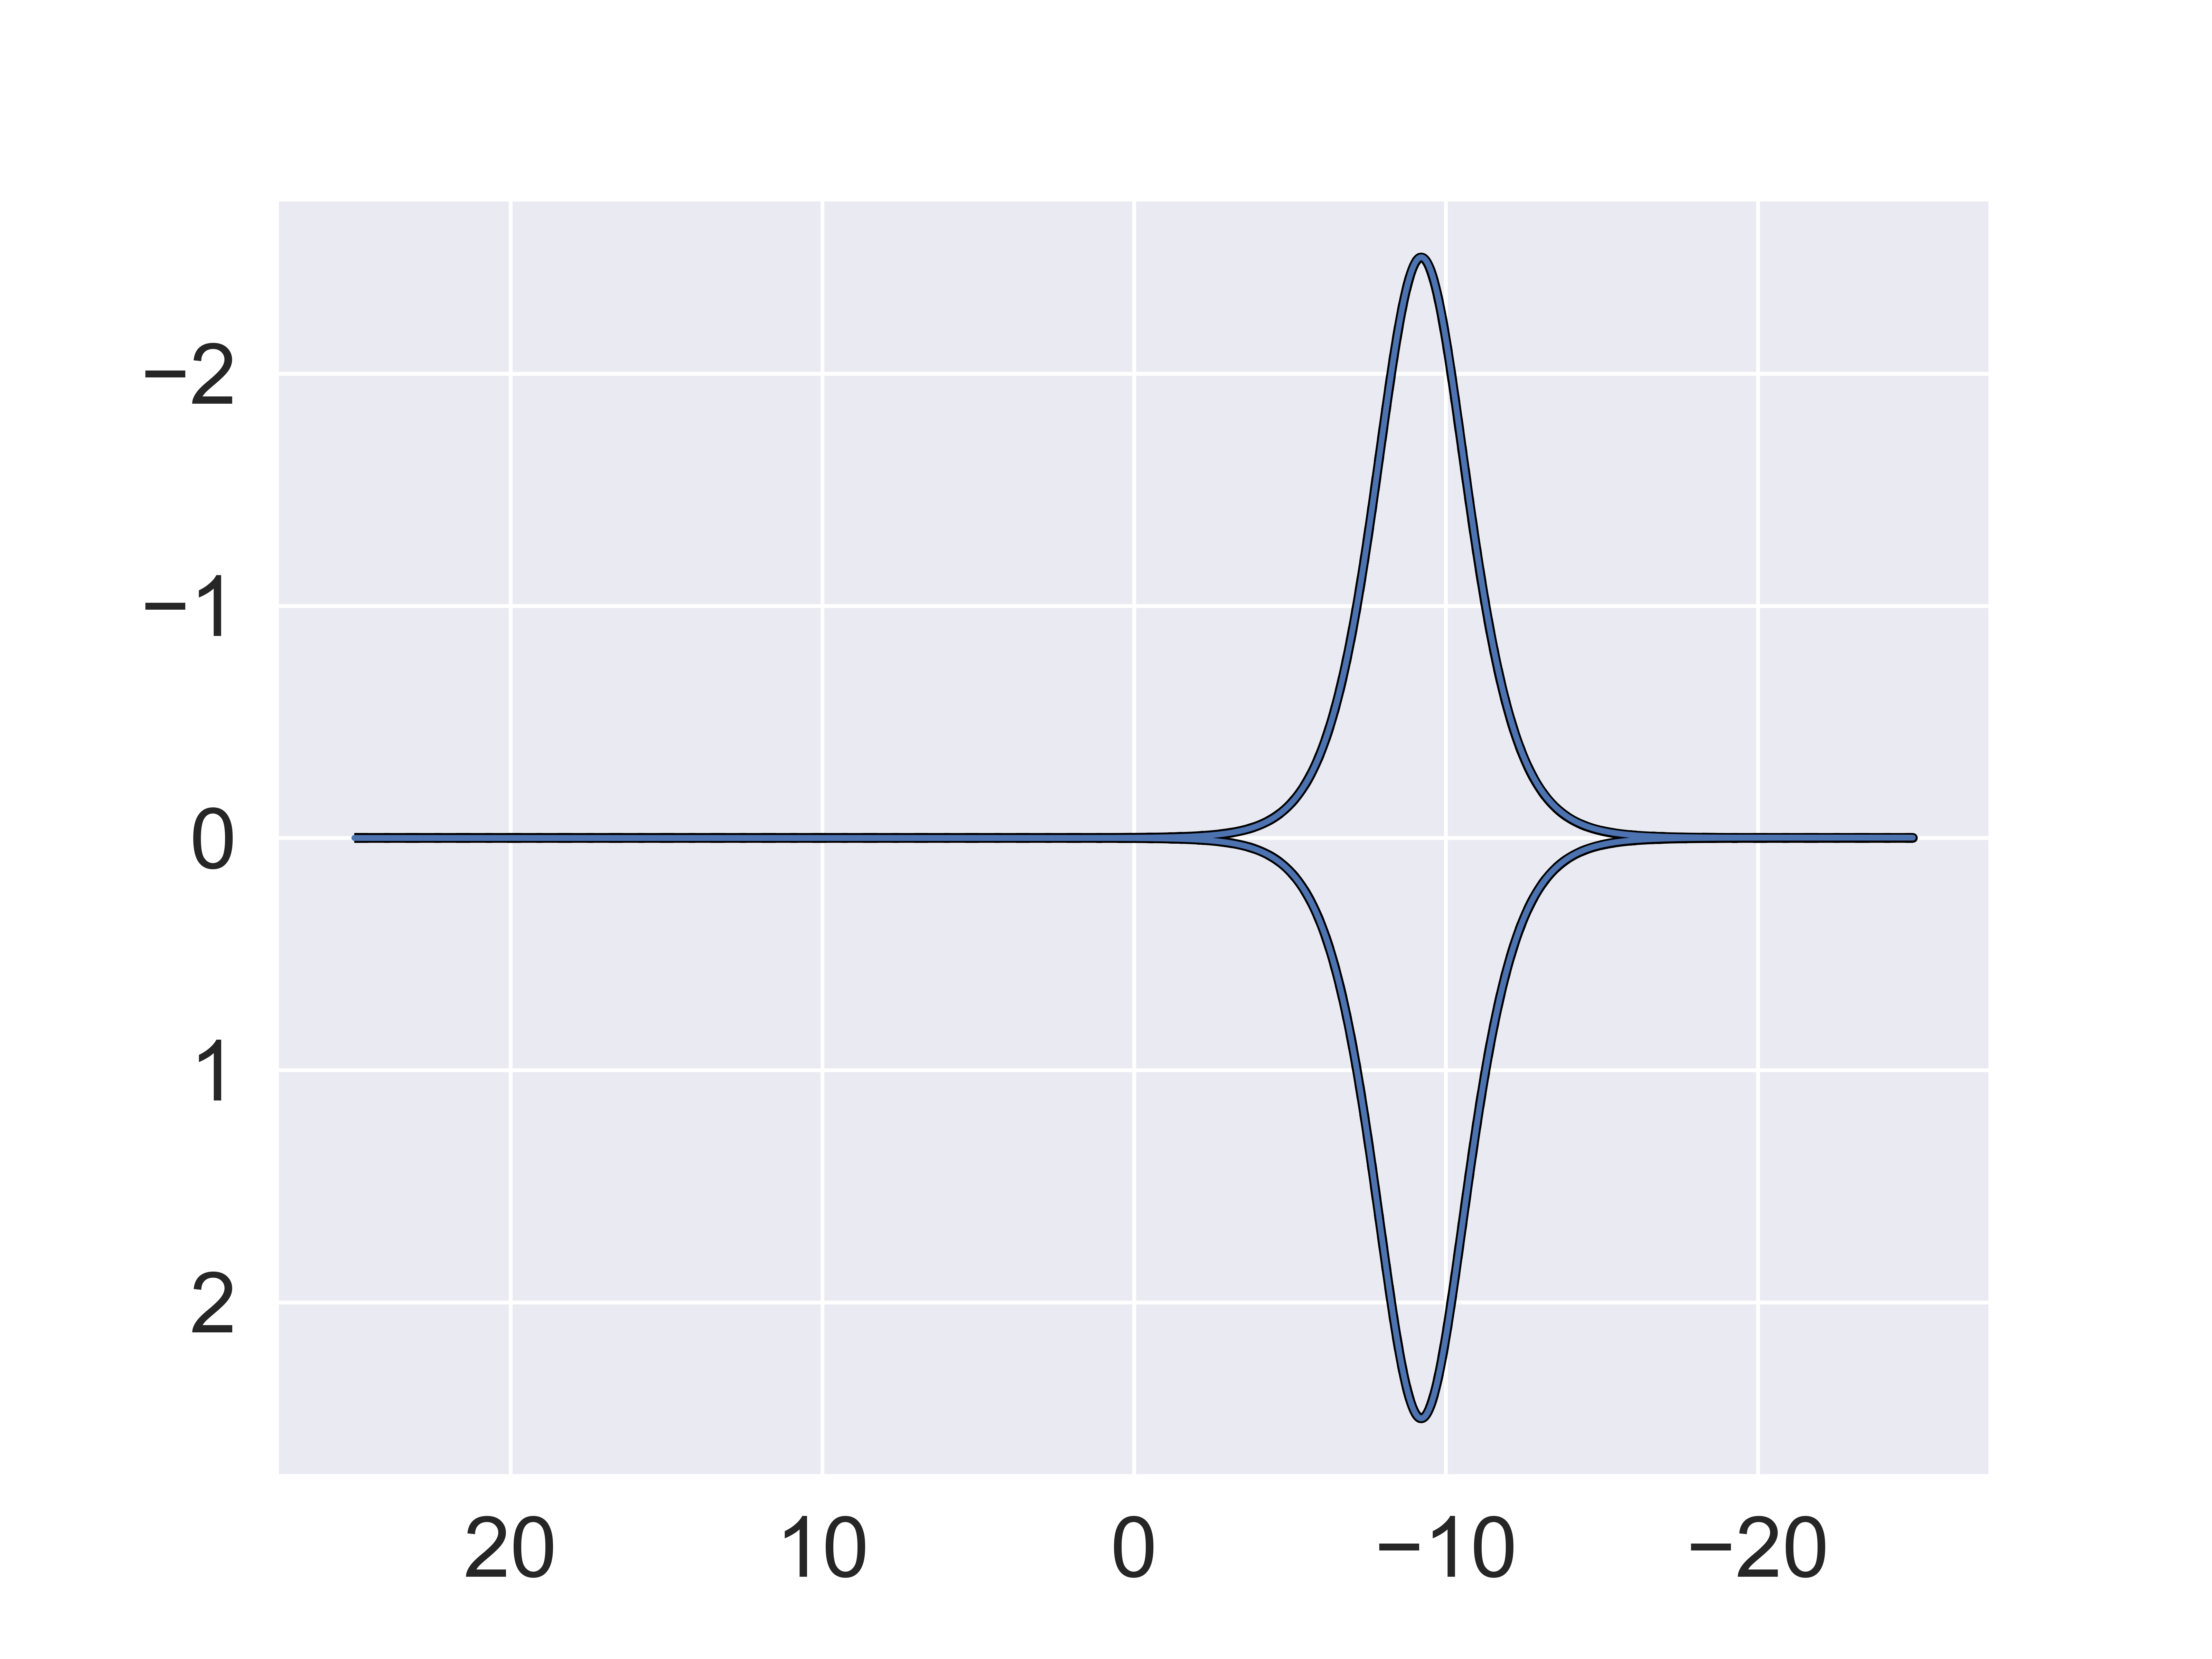
\includegraphics[width=0.5\textwidth]{figures/8-analytical.png}
  \caption[Verification against the monolayer analytical
  solution]{Voltammogram for a pure monolayer with a reversible adsorbed
    redox couple. The numerical solution (solid) matches the analytical
  current~\cref{eq:ads-monolayer-analytical} (dashed).}
  \label{fig:ads-verification}
\end{figure}

\subsection{Posterior Distributions}\label{sec:ads-posteriors}

\Cref{fig:ads-corner} shows pairwise marginal posteriors from NUTS
(2\,800 samples) and RWMH (40\,000 samples) under equal computational
budgets. Both samplers recover the true parameter values.
$\theta_f^{\mathrm{sol}}$ omitted for brevity.

The off-diagonal panels reveal the correlation structure.
$\alpha^{\mathrm{sol}}$ and $K_0^{\mathrm{sol}}$ are correlated due to
the kinetic trade-off in the Butler--Volmer equation, as in the
lower-dimensional cases; the same holds for $\alpha^{\mathrm{ads}}$ and
$K_0^{\mathrm{ads}}$. The adsorption and desorption rate constants for
each species are also correlated: the Langmuir terms
in~\cref{eq:ads-coverage-ode,eq:ads-bc} depend on these constants
primarily through the equilibrium ratio
$K_{\mathrm{ads}}^{j}/K_{\mathrm{des}}^{j}$, which sets the surface
coverage at steady state. Increasing both constants by the same factor
leaves this ratio nearly unchanged, producing a similar voltammogram.
The posterior is therefore elongated along the direction in which the
ratio is constant -- visible in the corner plot as diagonal contours
in the $K_{\mathrm{ads}}^{j}$ vs $K_{\mathrm{des}}^{j}$ panels. This
geometry makes sampling harder: moving along the ridge is easy, but
resolving the narrow cross-section requires precise steps, reducing
efficiency for both samplers as we quantify in \cref{sec:ads-ess}.
Despite these correlations, both samplers resolve the individual rate
constants.

\begin{figure}[ht]
  \centering
  \includegraphics[width=1.00\textwidth]{figures/8-corner.png}
  \caption[Pairwise posteriors for the adsorption
  reaction]{Pairwise marginal posteriors for the adsorption
    reaction. NUTS (blue) and RWMH (orange) are overlaid; dashed lines
    indicate the true parameter values. $\theta_f^{\mathrm{sol}}$
  omitted for brevity}
  \label{fig:ads-corner}
\end{figure}

That both samplers recover the true parameters -- despite inference
using the backward implicit linearisation rather than the Newton solver
that generated the data -- confirms that the
approximation~\cref{eq:ads-britz} does not introduce systematic bias at
this noise level.

\Cref{fig:ads-current-fit} overlays the posterior-mean voltammogram
with the true current. The 95\% credible interval is tight throughout
the sweep.

\begin{figure}[ht]
  \centering
  \includegraphics[width=0.7\textwidth]{figures/8-current-fit.png}
  \caption[Current fit for the adsorption reaction]{Posterior-mean
    voltammogram (solid) with 95\% credible interval (shaded) against
  the true current (dashed) and noisy data (points).}
  \label{fig:ads-current-fit}
\end{figure}

\subsection{Sampling Efficiency}\label{sec:ads-ess}

\Cref{fig:ads-ess} compares ESS growth for NUTS and RWMH on a
normalised cost axis. \Cref{tab:ads-ess} reports the final values with
NUTS/RWMH ratios. The results split into two groups. For the
solution-phase and adsorbed electron-transfer parameters
($\alpha^{\mathrm{sol}}$, $K_0^{\mathrm{sol}}$,
  $\theta_f^{\mathrm{sol}}$, $\alpha^{\mathrm{ads}}$,
$K_0^{\mathrm{ads}}$), the ratios are $4.0$--$4.8\times$, continuing
the upward trend from $1.5$--$2.4\times$ in three dimensions
(\cref{sec:hmc-results}) and $2.7$--$3.6\times$ in seven
(\cref{sec:het-ess}). For the adsorption/desorption rate constants the
ratios are lower, $2.3$--$2.6\times$: the elongated posterior geometry
described in \cref{sec:ads-posteriors} reduces the advantage of
gradient-based proposals, since both samplers struggle to resolve the
narrow cross-section of the ridge.

\begin{table}[ht]
  \centering
  \begin{tabular}{lccccccccc}
    \hline
    & $\alpha^{\mathrm{sol}}$ & $K_0^{\mathrm{sol}}$ & $\theta_f^{\mathrm{sol}}$
    & $\alpha^{\mathrm{ads}}$ & $K_0^{\mathrm{ads}}$
    & $K_{\mathrm{ads}}^{\mathrm{A}}$
    & $K_{\mathrm{des}}^{\mathrm{A}}$
    & $K_{\mathrm{ads}}^{\mathrm{B}}$
    & $K_{\mathrm{des}}^{\mathrm{B}}$ \\
    \hline
    NUTS & 4860.8 & 5527.5 & 4402.0 & 4707.2 & 5334.7 & 3451.7 &
    3319.6 & 3807.2 & 3501.9
    \\
    RWMH & 1185.0 & 1139.9 & 1113.7 & 1160.2 & 1311.9 & 1484.3 &
    1405.7 & 1439.8 & 1493.0
    \\
    Ratio & 4.1 & 4.8 & 4.0 & 4.1 & 4.1 & 2.3 & 2.4 & 2.6 & 2.3 \\
    \\
    \hline
  \end{tabular}
  \caption[ESS for the adsorption reaction]{Effective sample size for
    each parameter for 40\,000 RWMH samples and 2\,800 NUTS samples at
  equal sampling runtime, with NUTS/RWMH ratio.}
  \label{tab:ads-ess}
\end{table}

\begin{figure}[ht]
  \centering
  \includegraphics[width=0.95\textwidth]{figures/8-ess.png}
  \caption[ESS comparison for the adsorption reaction]{Effective
    sample size as a function of sample proportion for each parameter.
    NUTS (blue) accumulates independent samples at a higher rate than
  RWMH (orange) across all nine parameters.}
  \label{fig:ads-ess}
\end{figure}

\chapter{Conclusion}\label{ch:conclusions}
%TODO: Further work section here as well


\addcontentsline{toc}{chapter}{Bibliography}
\bibliography{references}
\bibliographystyle{plain}

\end{document}
